\documentclass[11pt,a4paper,oneside]{book}
\usepackage[utf8]{inputenc}
\usepackage[margin=1.8cm, top=2.2cm, bottom=2.2cm]{geometry}
\usepackage{amsmath,amssymb,amsfonts}
\usepackage{booktabs}
\usepackage{array}
\usepackage{xcolor}
\usepackage{tikz}
\usepackage{titlesec}
\usepackage{fancyhdr}
\usepackage{tcolorbox}
\tcbuselibrary{skins,breakable}
\usepackage{hyperref}
\usepackage{enumitem}
\usepackage{setspace}

\usetikzlibrary{shapes.gates.logic.US,positioning,calc,arrows.meta}

% Line Spacing and Paragraph Spacing
\setstretch{1.22}
\setlength{\parskip}{0.5em}
\setlength{\parindent}{0pt}
\setlist[enumerate]{itemsep=0.35em, topsep=0.35em, parsep=0.15em}
\setlist[itemize]{itemsep=0.35em, topsep=0.35em, parsep=0.15em}

% Custom Color Palette
\definecolor{primarydark}{HTML}{0f172a}
\definecolor{secondaryblue}{HTML}{1e3a8a}
\definecolor{accentindigo}{HTML}{4338ca}
\definecolor{boxbg}{HTML}{f8fafc}
\definecolor{boxborder}{HTML}{cbd5e1}
\definecolor{alertborder}{HTML}{3b82f6}
\definecolor{ansbg}{HTML}{f0fdf4}
\definecolor{ansborder}{HTML}{16a34a}
\definecolor{diagbg}{HTML}{ffffff}
\definecolor{diagborder}{HTML}{4338ca}

% Typography & Headings
\titleformat{\chapter}[display]
{\normalfont\huge\bfseries\color{primarydark}}{\chaptertitlename\ \thechapter}{12pt}{\Huge}
\titleformat{\section}
{\normalfont\Large\bfseries\color{secondaryblue}}{\thesection}{1em}{}
\titleformat{\subsection}
{\normalfont\large\bfseries\color{accentindigo}}{\thesubsection}{1em}{}

% Headers & Footers
\pagestyle{fancy}
\fancyhf{}
\fancyhead[L]{\small\bfseries\sffamily\color{secondaryblue} Electronic Devices \& Circuits (EX 151) --- IOE Master Solutions}
\fancyhead[R]{\small\sffamily\color{gray} Tribhuvan University}
\fancyfoot[C]{\sffamily\bfseries\thepage}
\renewcommand{\headrulewidth}{0.6pt}

% Custom TColorBoxes with Enhanced Internal Spacing
\newtcolorbox{questionbox}[1]{
  colback=boxbg,
  colframe=alertborder,
  coltitle=white,
  fonttitle=\bfseries\sffamily,
  title={#1},
  arc=2.5mm,
  boxrule=1pt,
  boxsep=5pt,
  top=7pt,
  bottom=7pt,
  left=8pt,
  right=8pt,
  before upper={\setstretch{1.2}},
  breakable,
  enhanced
}

\newtcolorbox{answerbox}{
  colback=ansbg,
  colframe=ansborder,
  coltitle=white,
  fonttitle=\bfseries\sffamily,
  title={Final Verified Result},
  arc=2.5mm,
  boxrule=1pt,
  boxsep=5pt,
  top=6pt,
  bottom=6pt,
  left=8pt,
  right=8pt,
  before upper={\setstretch{1.2}},
  breakable,
  enhanced
}

\newtcolorbox{schematicbox}[1]{
  colback=diagbg,
  colframe=diagborder,
  coltitle=white,
  fonttitle=\bfseries\sffamily,
  title={Circuit Schematic / Analysis Diagram: #1},
  arc=2.5mm,
  boxrule=1pt,
  boxsep=6pt,
  top=8pt,
  bottom=8pt,
  left=8pt,
  right=8pt,
  breakable,
  enhanced
}

\begin{document}

% Title Page
\begin{titlepage}
  \centering
  \vspace*{1.5cm}
  {\Huge \bfseries \color{primarydark} TRIBHUVAN UNIVERSITY\par}
  \vspace{0.4cm}
  {\Large \bfseries \color{secondaryblue} INSTITUTE OF ENGINEERING (IOE)\par}
  \vspace{1.5cm}
  {\Huge \bfseries \color{accentindigo} ELECTRONIC DEVICES \& CIRCUITS\par}
  \vspace{0.5cm}
  {\LARGE Course Code: EX 151 / EX 501 / CT 501\par}
  \vspace{0.3cm}
  {\large BE Electronics, Information and Communication (BEI) \& BE Computer (BCT)\par}
  \vspace{2.0cm}
  
  \begin{tcolorbox}[colback=boxbg,colframe=alertborder,width=0.88\textwidth,arc=3mm,center]
    \centering
    \Large \textbf{Comprehensive Master Examination Solutions}\par
    \vspace{0.3cm}
    \normalsize \textit{Complete step-by-step mathematical derivations, small-signal AC models, DC biasing calculations, power amplifier efficiencies, oscillator analyses, and high-precision TikZ schematics for all exam sittings.}
  \end{tcolorbox}
  
  \vfill
  {\large \textbf{Academic Exam Papers Covered:}\par}
  {\normalsize 2083 Baishakh $\cdot$ 2082 Bhadra $\cdot$ 2082 Baishakh $\cdot$ 2081 Ashwin\par}
  \vspace{1.0cm}
  {\small IOE Examination Reference Edition $\cdot$ August 2026\par}
\end{titlepage}

\tableofcontents
\newpage

\chapter{2083 Baishakh Examination Solutions}

\section*{Examination Overview}
\begin{tabular}{@{}ll@{}}
\textbf{Level:} Bachelor in Engineering (BE) & \textbf{Full Marks:} 60 \\
\textbf{Programme:} BEI, BCT & \textbf{Pass Marks:} 24 \\
\textbf{Year / Part:} I / II & \textbf{Time:} 3 Hours \\
\textbf{Subject:} Electronic Devices \& Circuits (ENEX 151) & \textbf{Examination Type:} Back (New Course) \\
\end{tabular}

\vspace{0.6cm}
\hrule
\vspace{0.6cm}

% =========================================================================
% QUESTION 1
% =========================================================================
\subsection{Question 1: BJT vs. FET Conduction \& Common Collector Amplifier Design [1 + 5 = 6 Marks]}
\begin{questionbox}{Problem Statement (2083 Baishakh, Q1)}
Why BJT is bipolar and FET is unipolar? Design $\beta$-independent type DC biased common collector amplifier. Given parameters are: $V_{CC} = 20\text{ V}, I_C = 2\text{ mA}$, and $\beta = 100$. Use firm biasing method.
\end{questionbox}

\paragraph{Part (a): Bipolar vs. Unipolar Operating Mechanism [1 Mark]}
\begin{itemize}[leftmargin=1.5em]
  \item \textbf{BJT is Bipolar:} Its current conduction relies simultaneously on \textbf{both majority and minority charge carriers} (free electrons and holes) flowing across two $p$-$n$ junctions (emitter-base and collector-base).
  \item \textbf{FET is Unipolar:} Electric conduction takes place exclusively through a continuous channel containing \textbf{only one type of charge carrier} (electrons in n-channel, holes in p-channel) modulated by an electric field with zero minority carrier participation.
\end{itemize}

\paragraph{Part (b): $\beta$-Independent Common Collector (Emitter Follower) Design [5 Marks]}
\begin{enumerate}[leftmargin=1.5em]
  \item \textbf{Emitter Bias Voltage Selection ($V_{EQ}$):}
  To allow maximum symmetrical undistorted AC output voltage swing without premature clipping:
  \[
  V_{EQ} = \frac{V_{CC}}{2} = \frac{20\text{ V}}{2} = \mathbf{10.0\text{ V}}
  \]
  \item \textbf{Emitter Resistor ($R_E$):}
  Since $I_E \approx I_C = 2.0\text{ mA}$:
  \[
  R_E = \frac{V_{EQ}}{I_E} = \frac{10.0\text{ V}}{2.0\text{ mA}} = 5.0\text{ k}\Omega \quad (\text{Select standard } R_E = \mathbf{5.1\text{ k}\Omega})
  \]
  \item \textbf{Base DC Voltage ($V_B$):}
  \[
  V_B = V_{EQ} + V_{BE} = 10.0\text{ V} + 0.7\text{ V} = \mathbf{10.7\text{ V}}
  \]
  \item \textbf{Firm Biasing Method ($I_{\text{bleed}} = 10 I_B$):}
  \[
  I_B = \frac{I_C}{\beta} = \frac{2.0\text{ mA}}{100} = 0.02\text{ mA} = 20\ \mu\text{A}
  \]
  \[
  I_{\text{bleed}} = 10 \times I_B = 10 \times 0.02\text{ mA} = \mathbf{0.20\text{ mA}}
  \]
  \item \textbf{Voltage Divider Resistors ($R_1, R_2$):}
  \[
  R_2 = \frac{V_B}{I_{\text{bleed}}} = \frac{10.7\text{ V}}{0.20\text{ mA}} = 53.5\text{ k}\Omega \quad (\text{Select standard } R_2 = \mathbf{56\text{ k}\Omega})
  \]
  \[
  R_1 = \frac{V_{CC} - V_B}{I_{\text{bleed}} + I_B} = \frac{20\text{ V} - 10.7\text{ V}}{0.20\text{ mA} + 0.02\text{ mA}} = \frac{9.3\text{ V}}{0.22\text{ mA}} = 42.27\text{ k}\Omega \quad (\text{Select standard } R_1 = \mathbf{43\text{ k}\Omega})
  \]
  \item \textbf{$\beta$-Independency Verification:}
  \[
  R_{\text{th}} = R_1 \parallel R_2 = 43\text{ k}\Omega \parallel 56\text{ k}\Omega = \frac{43 \times 56}{43 + 56} = \mathbf{24.32\text{ k}\Omega}
  \]
  Firm bias stability criterion: $R_{\text{th}} \le 0.1(1+\beta)R_E = 0.1(101)(5.1\text{ k}\Omega) = 51.5\text{ k}\Omega \implies 24.32\text{ k}\Omega < 51.5\text{ k}\Omega \quad \checkmark$
\end{enumerate}

\begin{schematicbox}{Designed $\beta$-Independent Common Collector (Emitter Follower) Circuit}
\centering
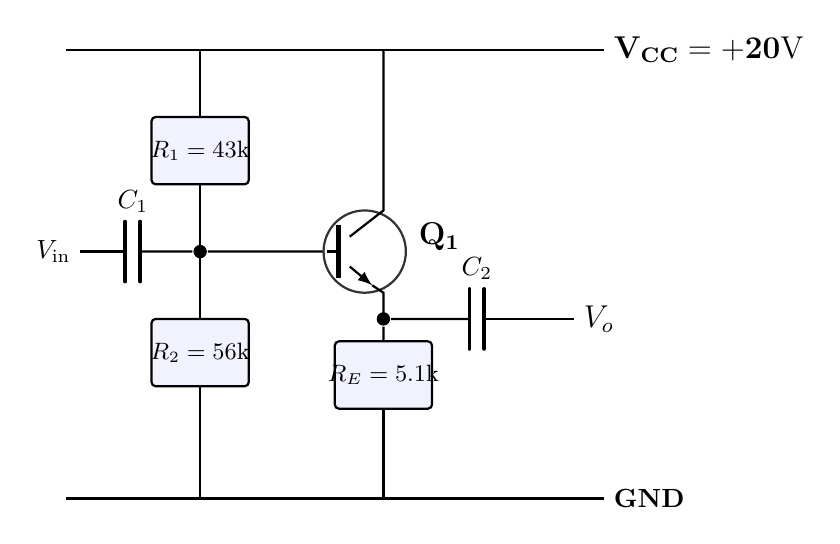
\begin{tikzpicture}[scale=0.95, transform shape]
  % Rails
  \draw[thick] (0, 5.2) -- (7.2, 5.2) node[right] {\large $\mathbf{V_{CC} = +20\text{V}}$};
  \draw[thick] (0, -0.8) -- (7.2, -0.8) node[right] {\textbf{GND}};

  % Divider R1 and R2
  \draw[thick] (1.8, 5.2) -- (1.8, 4.3);
  \draw[thick, fill=blue!5, rounded corners=1.5pt] (1.15, 3.4) rectangle (2.45, 4.3) node[midway] {\small $R_1=43\text{k}$};
  \draw[thick] (1.8, 3.4) -- (1.8, 2.5) node[circle, fill, inner sep=1.8pt] (vb) {};
  \draw[thick] (1.8, 2.5) -- (1.8, 1.6);
  \draw[thick, fill=blue!5, rounded corners=1.5pt] (1.15, 0.7) rectangle (2.45, 1.6) node[midway] {\small $R_2=56\text{k}$};
  \draw[thick] (1.8, 0.7) -- (1.8, -0.8);

  % Input coupling capacitor C1
  \draw[thick] (0.2, 2.5) node[left] {$V_{\text{in}}$} -- (0.8, 2.5);
  \draw[line width=1.4pt, line cap=round] (0.8, 2.1) -- (0.8, 2.9);
  \draw[line width=1.4pt, line cap=round] (1.0, 2.1) -- (1.0, 2.9);
  \node[above] at (0.9, 2.9) {$C_1$};
  \draw[thick] (1.0, 2.5) -- (vb);

  % Transistor Q1 (NPN)
  \draw[thick] (vb) -- (3.5, 2.5);
  \draw[draw=black!80, fill=white, thick] (4.0, 2.5) circle (0.55cm);
  \draw[line width=1.6pt] (3.65, 2.15) -- (3.65, 2.85); % Base
  \draw[thick] (3.5, 2.5) -- (3.65, 2.5);
  \draw[thick] (3.8, 2.7) -- (4.25, 3.05) -- (4.25, 5.2); % Collector directly to VCC
  \draw[thick, ->, >=latex] (3.8, 2.3) -- (4.1, 2.05); % Emitter
  \draw[thick] (4.1, 2.05) -- (4.25, 1.95) -- (4.25, 1.6) node[circle, fill, inner sep=1.8pt] (ve) {};
  \node[right=0.2cm] at (4.4, 2.7) {\large $\mathbf{Q_1}$};

  % Emitter Resistor RE
  \draw[thick] (ve) -- (4.25, 1.3);
  \draw[thick, fill=blue!5, rounded corners=1.5pt] (3.6, 0.4) rectangle (4.9, 1.3) node[midway] {\small $R_E=5.1\text{k}$};
  \draw[thick] (4.25, 0.4) -- (4.25, -0.8);

  % Output coupling capacitor C2
  \draw[thick] (ve) -- (5.4, 1.6);
  \draw[line width=1.4pt, line cap=round] (5.4, 1.2) -- (5.4, 2.0);
  \draw[line width=1.4pt, line cap=round] (5.6, 1.2) -- (5.6, 2.0);
  \node[above] at (5.5, 2.0) {$C_2$};
  \draw[thick] (5.6, 1.6) -- (6.8, 1.6) node[right] {\large $V_o$};
\end{tikzpicture}
\end{schematicbox}

\begin{answerbox}
$$\mathbf{R_1 = 43\text{ k}\Omega, \quad R_2 = 56\text{ k}\Omega, \quad R_E = 5.1\text{ k}\Omega, \quad V_{EQ} = 10\text{ V}, \quad I_{CQ} = 2.0\text{ mA}}$$
\end{answerbox}

\vspace{0.6cm}

% =========================================================================
% QUESTION 2
% =========================================================================
\subsection{Question 2: Role of Bypass Capacitor \& Common Base AC Parameters [2 + 5 = 7 Marks]}
\begin{questionbox}{Problem Statement (2083 Baishakh, Q2)}
Explain the role of bypass capacitor in amplifier circuits. Draw the small signal equivalent circuit of a common base amplifier circuit and find its input impedance, output impedance and voltage gain.
\end{questionbox}

\paragraph{Part (a): Role of Bypass Capacitor [2 Marks]}
\begin{itemize}[leftmargin=1.5em]
  \item In a BJT amplifier, the emitter resistor $R_E$ provides crucial DC operating point stability against temperature variations and $\beta$ changes.
  \item However, for AC signals, an unbypassed $R_E$ introduces negative series current feedback which drastically reduces the AC voltage gain ($A_v \approx -R_C/R_E$).
  \item Connecting a **bypass capacitor ($C_E$)** in parallel with $R_E$ provides a near zero-impedance AC short-circuit path ($X_{C_E} = \frac{1}{2\pi f C_E} \approx 0$) to ground at signal frequencies, eliminating AC negative feedback and maximizing voltage gain ($A_v \approx -R_C/r_e$).
\end{itemize}

\paragraph{Part (b): Common Base Small-Signal Equivalent Model [5 Marks]}
\begin{schematicbox}{Small-Signal $r_e$ Model of Common Base (CB) Amplifier}
\centering
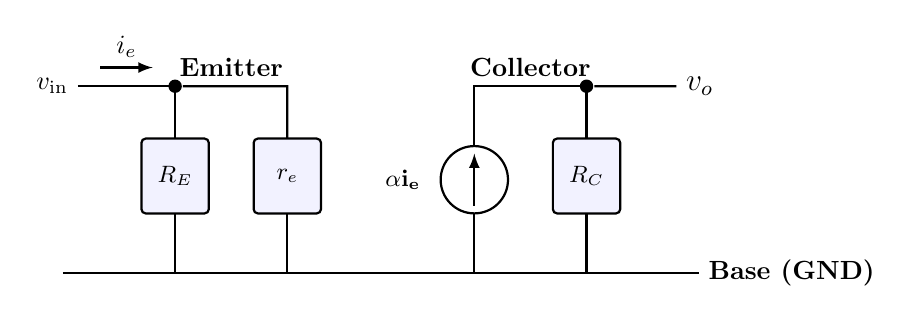
\begin{tikzpicture}[scale=0.95, transform shape]
  % Common Base Ground Rail
  \draw[thick] (0, 0) -- (8.5, 0) node[right] {\textbf{Base (GND)}};

  % Input Terminal at Emitter (Left)
  \draw[thick] (0.2, 2.5) node[left] {$v_{\text{in}}$} -- (1.5, 2.5) node[circle, fill, inner sep=1.8pt] (e_node) {};
  \draw[thick, ->, >=latex] (0.5, 2.75) -- (1.2, 2.75) node[midway, above] {$i_e$};

  % Emitter Biasing Resistor RE
  \draw[thick] (1.5, 2.5) -- (1.5, 1.8);
  \draw[thick, fill=blue!5, rounded corners=1.5pt] (1.05, 0.8) rectangle (1.95, 1.8) node[midway] {\small $R_E$};
  \draw[thick] (1.5, 0.8) -- (1.5, 0);

  % Dynamic Emitter Resistance re
  \draw[thick] (e_node) -- (3.0, 2.5) -- (3.0, 1.8);
  \draw[thick, fill=blue!5, rounded corners=1.5pt] (2.55, 0.8) rectangle (3.45, 1.8) node[midway] {\small $r_e$};
  \draw[thick] (3.0, 0.8) -- (3.0, 0);
  \node[above] at (2.25, 2.5) {\textbf{Emitter}};

  % Dependent Collector Current Source alpha * ie (Right branch, pointing UP to collector)
  \draw[thick] (5.5, 0) -- (5.5, 0.8);
  \draw[thick] (5.5, 1.25) circle (0.45cm);
  \draw[thick, ->, >=latex] (5.5, 0.9) -- (5.5, 1.6);
  \node[left=0.15cm] at (5.05, 1.25) {\small $\mathbf{\alpha i_e}$};
  \draw[thick] (5.5, 1.7) -- (5.5, 2.5) -- (7.0, 2.5) node[circle, fill, inner sep=1.8pt] (c_node) {};
  \node[above] at (6.25, 2.5) {\textbf{Collector}};

  % Collector Resistor RC
  \draw[thick] (7.0, 2.5) -- (7.0, 1.8);
  \draw[thick, fill=blue!5, rounded corners=1.5pt] (6.55, 0.8) rectangle (7.45, 1.8) node[midway] {\small $R_C$};
  \draw[thick] (7.0, 0.8) -- (7.0, 0);

  % Output Node
  \draw[thick] (c_node) -- (8.2, 2.5) node[right] {\large $v_o$};
\end{tikzpicture}
\end{schematicbox}

\begin{enumerate}[leftmargin=1.5em]
  \item \textbf{Input Impedance ($Z_{\text{in}}$):}
  Looking into the emitter terminal with base grounded:
  \[
  Z_{\text{in}} = R_E \parallel r_e \approx \mathbf{r_e = \frac{V_T}{I_E}} \quad (\text{very low, typically } 10\ \Omega - 50\ \Omega)
  \]
  \item \textbf{Output Impedance ($Z_{\text{out}}$):}
  Looking back from the collector with $v_{\text{in}} = 0 \implies i_e = 0$:
  \[
  Z_{\text{out}} = R_C \parallel r_o \approx \mathbf{R_C} \quad (\text{high})
  \]
  \item \textbf{Voltage Gain ($A_v$):}
  \[
  v_o = -(-\alpha i_e)(R_C \parallel R_L) = \alpha i_e (R_C \parallel R_L), \qquad v_{\text{in}} = i_e r_e
  \]
  \[
  \mathbf{A_v = \frac{v_o}{v_{\text{in}}} = \frac{\alpha (R_C \parallel R_L)}{r_e} \approx +\frac{R_C \parallel R_L}{r_e}} \quad (\text{Non-inverting, } 0^\circ \text{ phase shift})
  \]
  \item \textbf{Current Gain ($A_i$):}
  \[
  \mathbf{A_i = \frac{i_o}{i_e} = -\alpha \approx -1}
  \]
\end{enumerate}

\begin{answerbox}
$$\mathbf{Z_{\text{in}} \approx r_e = \frac{V_T}{I_E}, \qquad Z_{\text{out}} \approx R_C, \qquad A_v = +\frac{\alpha(R_C \parallel R_L)}{r_e}, \qquad A_i = -\alpha \approx -1}$$
\end{answerbox}

\vspace{0.6cm}

% =========================================================================
% QUESTION 3
% =========================================================================
\subsection{Question 3: N-Channel Depletion-Type MOSFET [6 Marks]}
\begin{questionbox}{Problem Statement (2083 Baishakh, Q3)}
Describe the construction and working principle of N Channel D-MOSFET with the help of characteristic curves and mathematical expressions.
\end{questionbox}

\paragraph{1. Physical Construction:}
Fabricated on a p-type silicon substrate with two heavily doped $n^+$ Source and Drain regions, physically connected by an initial pre-diffused n-channel. The Gate electrode is completely insulated from the channel by an ultrathin silicon dioxide ($\text{SiO}_2$) dielectric layer ($R_{\text{in}} > 10^{12}\ \Omega$).

\begin{schematicbox}{Transfer and Drain Characteristics of N-Channel D-MOSFET}
\centering
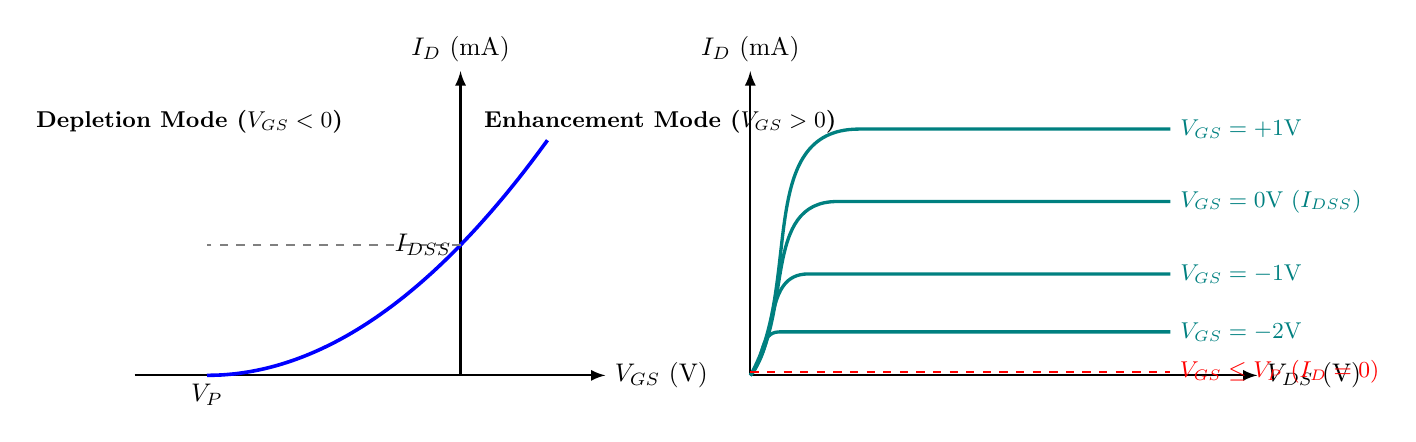
\begin{tikzpicture}[scale=0.92, transform shape]
  % Transfer Characteristics (left)
  \draw[thick, ->, >=latex] (-4.5, 0) -- (2.0, 0) node[right] {$V_{GS}\ (\text{V})$};
  \draw[thick, ->, >=latex] (0, 0) -- (0, 4.2) node[above] {$I_D\ (\text{mA})$};
  \draw[domain=-3.5:1.2, smooth, variable=\x, line width=1.3pt, blue] plot ({\x}, {1.8*(1 + \x/3.5)^2});
  \node[below] at (-3.5, 0) {$V_P$};
  \draw[dashed, gray] (0, 1.8) -- (-3.5, 1.8);
  \node[left] at (0, 1.8) {$I_{DSS}$};
  \node[left] at (-1.5, 3.5) {\small\textbf{Depletion Mode ($V_{GS}<0$)}};
  \node[right] at (0.2, 3.5) {\small\textbf{Enhancement Mode ($V_{GS}>0$)}};

  % Drain Characteristics (right)
  \draw[thick, ->, >=latex] (4.0, 0) -- (11.0, 0) node[right] {$V_{DS}\ (\text{V})$};
  \draw[thick, ->, >=latex] (4.0, 0) -- (4.0, 4.2) node[above] {$I_D\ (\text{mA})$};
  \draw[line width=1.2pt, teal] (4.0, 0) to[out=60, in=180] (5.5, 3.4) -- (9.8, 3.4) node[right] {\small $V_{GS} = +1\text{V}$};
  \draw[line width=1.2pt, teal] (4.0, 0) to[out=55, in=180] (5.2, 2.4) -- (9.8, 2.4) node[right] {\small $V_{GS} = 0\text{V}\ (I_{DSS})$};
  \draw[line width=1.2pt, teal] (4.0, 0) to[out=50, in=180] (4.8, 1.4) -- (9.8, 1.4) node[right] {\small $V_{GS} = -1\text{V}$};
  \draw[line width=1.2pt, teal] (4.0, 0) to[out=45, in=180] (4.4, 0.6) -- (9.8, 0.6) node[right] {\small $V_{GS} = -2\text{V}$};
  \draw[thick, red, dashed] (4.0, 0.05) -- (9.8, 0.05) node[right] {\small $V_{GS} \le V_P\ (I_D=0)$};
\end{tikzpicture}
\end{schematicbox}

\paragraph{2. Working Principle \& Modes of Operation:}
\begin{enumerate}[leftmargin=1.5em]
  \item \textbf{Depletion Mode ($V_{GS} < 0$):} Negative gate voltage repels electrons out of the n-channel, creating a depletion region and reducing drain current below $I_{DSS}$. At $V_{GS} = V_P$ (pinch-off), the channel is completely closed ($I_D = 0$).
  \item \textbf{Enhancement Mode ($V_{GS} > 0$):} Positive gate voltage attracts additional free electrons into the channel, widening it and increasing drain current above $I_{DSS}$.
\end{enumerate}

\paragraph{3. Governing Shockley Equation:}
\[
\mathbf{I_D = I_{DSS}\left(1 - \frac{V_{GS}}{V_P}\right)^2 \quad \text{for } V_{DS} \ge V_{GS} - V_P}
\]
\[
\mathbf{g_m = \left.\frac{\partial I_D}{\partial V_{GS}}\right|_{V_{DS}} = \frac{2I_{DSS}}{|V_P|}\left(1 - \frac{V_{GS}}{V_P}\right) = g_{m0}\left(1 - \frac{V_{GS}}{V_P}\right)}
\]

\begin{answerbox}
$$\mathbf{I_D = I_{DSS}\left(1 - \frac{V_{GS}}{V_P}\right)^2 \quad \text{valid in both Depletion } (V_{GS}<0) \text{ and Enhancement } (V_{GS}>0) \text{ modes}}$$
\end{answerbox}

\vspace{0.6cm}

% =========================================================================
% QUESTION 4
% =========================================================================
\subsection{Question 4: JFET Voltage Divider Bias Analysis [7 Marks]}
\begin{questionbox}{Problem Statement (2083 Baishakh, Q4)}
Find $I_D$ and $V_{DS}$ for the given circuit. Given parameters: $V_P = -4\text{ V}$ and $I_{DSS} = 8\text{ mA}$.
Circuit values: $V_{DD} = +16\text{ V}, R_1 = 2.1\text{ M}\Omega, R_2 = 270\text{ k}\Omega, R_D = 2.4\text{ k}\Omega, R_S = 1.5\text{ k}\Omega$.
\end{questionbox}

\begin{schematicbox}{JFET Voltage-Divider Bias Circuit}
\centering
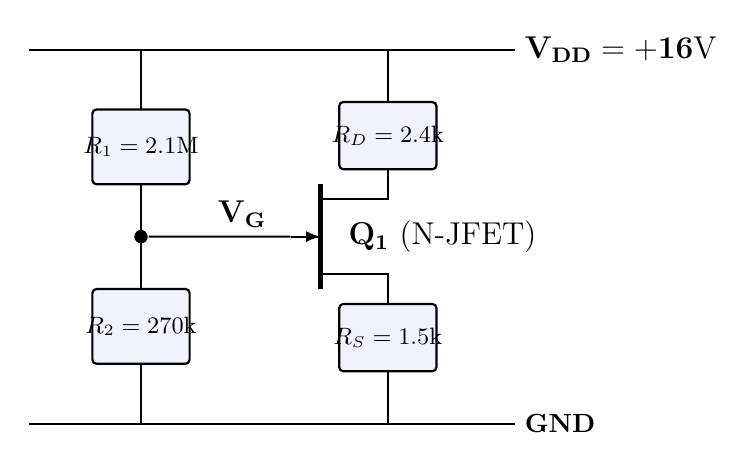
\begin{tikzpicture}[scale=0.95, transform shape]
  % Rails
  \draw[thick] (0, 5.0) -- (6.5, 5.0) node[right] {\large $\mathbf{V_{DD} = +16\text{V}}$};
  \draw[thick] (0, 0) -- (6.5, 0) node[right] {\textbf{GND}};

  % Gate Voltage Divider (R1 and R2)
  \draw[thick] (1.5, 5.0) -- (1.5, 4.2);
  \draw[thick, fill=blue!5, rounded corners=1.5pt] (0.85, 3.2) rectangle (2.15, 4.2) node[midway] {\small $R_1=2.1\text{M}$};
  \draw[thick] (1.5, 3.2) -- (1.5, 2.5) node[circle, fill, inner sep=1.8pt] (vg_node) {};
  \draw[thick] (1.5, 2.5) -- (1.5, 1.8);
  \draw[thick, fill=blue!5, rounded corners=1.5pt] (0.85, 0.8) rectangle (2.15, 1.8) node[midway] {\small $R_2=270\text{k}$};
  \draw[thick] (1.5, 0.8) -- (1.5, 0);

  % N-JFET Transistor
  \draw[thick] (vg_node) -- (3.5, 2.5);
  \draw[thick] (3.5, 2.5) -- (3.9, 2.5);
  \draw[line width=1.5pt] (3.9, 1.8) -- (3.9, 3.2); % Channel bar
  \draw[thick, ->, >=latex] (3.5, 2.5) -- (3.9, 2.5); % Inward arrow for N-JFET
  \node[left=0.2cm] at (3.5, 2.8) {\large $\mathbf{V_G}$};

  % Drain Branch (RD)
  \draw[thick] (3.9, 3.0) -- (4.8, 3.0) -- (4.8, 3.4);
  \draw[thick, fill=blue!5, rounded corners=1.5pt] (4.15, 3.4) rectangle (5.45, 4.3) node[midway] {\small $R_D=2.4\text{k}$};
  \draw[thick] (4.8, 4.3) -- (4.8, 5.0);

  % Source Branch (RS)
  \draw[thick] (3.9, 2.0) -- (4.8, 2.0) -- (4.8, 1.6);
  \draw[thick, fill=blue!5, rounded corners=1.5pt] (4.15, 0.7) rectangle (5.45, 1.6) node[midway] {\small $R_S=1.5\text{k}$};
  \draw[thick] (4.8, 0.7) -- (4.8, 0);
  \node[right=0.15cm] at (4.0, 2.5) {\large $\mathbf{Q_1}$ (N-JFET)};
\end{tikzpicture}
\end{schematicbox}

\paragraph{1. Thevenin Gate DC Voltage ($V_G$):}
Since the gate of a JFET draws negligible current ($I_G \approx 0$):
\[
V_G = V_{DD} \left(\frac{R_2}{R_1 + R_2}\right) = 16\text{ V} \times \left(\frac{270\text{ k}\Omega}{2100\text{ k}\Omega + 270\text{ k}\Omega}\right) = 16 \times \frac{270}{2370} = \mathbf{1.823\text{ V}}
\]

\paragraph{2. Gate-to-Source Voltage Equation ($V_{GS}$):}
Applying KVL around the gate-source loop:
\[
V_{GS} = V_G - I_D R_S = 1.823 - 1.5 I_D \quad (\text{with } I_D \text{ in mA and } R_S = 1.5\text{ k}\Omega)
\]

\paragraph{3. Solving via Shockley's Equation:}
\[
I_D = I_{DSS} \left(1 - \frac{V_{GS}}{V_P}\right)^2 = 8 \left(1 - \frac{1.823 - 1.5 I_D}{-4}\right)^2 = 8 \left(\frac{4 + 1.823 - 1.5 I_D}{4}\right)^2
\]
\[
I_D = \frac{8}{16} (5.823 - 1.5 I_D)^2 = 0.5 \left(33.907 - 17.469 I_D + 2.25 I_D^2\right)
\]
\[
2 I_D = 33.907 - 17.469 I_D + 2.25 I_D^2 \implies \mathbf{2.25 I_D^2 - 19.469 I_D + 33.907 = 0}
\]
Solving using the quadratic formula:
\[
I_D = \frac{19.469 \pm \sqrt{(-19.469)^2 - 4(2.25)(33.907)}}{2(2.25)} = \frac{19.469 \pm \sqrt{379.04 - 305.16}}{4.5} = \frac{19.469 \pm 8.595}{4.5}
\]
Two mathematical roots:
\begin{itemize}[leftmargin=1.5em]
  \item $I_{D1} = \frac{28.064}{4.5} = 6.236\text{ mA} \implies V_{GS1} = 1.823 - 1.5(6.236) = -7.53\text{ V} < V_P = -4\text{ V}$ (\textbf{Physically Invalid, beyond pinch-off}).
  \item $I_{D2} = \frac{10.874}{4.5} = \mathbf{2.416\text{ mA}} \implies V_{GS2} = 1.823 - 1.5(2.416) = \mathbf{-1.802\text{ V}}$ (\textbf{Physically Valid, in active channel region}).
\end{itemize}

\paragraph{4. Calculation of Drain-to-Source Voltage ($V_{DS}$):}
\[
V_{DS} = V_{DD} - I_D(R_D + R_S) = 16\text{ V} - 2.416\text{ mA} \times (2.4\text{ k}\Omega + 1.5\text{ k}\Omega) = 16 - 2.416(3.9) = \mathbf{6.576\text{ V}}
\]
\textbf{Pinch-Off Verification:}
\[
V_{DS} = 6.576\text{ V} \ge V_{GS} - V_P = -1.802\text{ V} - (-4.0\text{ V}) = 2.198\text{ V} \implies \text{Confirmed in Saturation Region!} \quad \checkmark
\]

\begin{answerbox}
$$\mathbf{I_D = 2.416\text{ mA}, \qquad V_{GS} = -1.802\text{ V}, \qquad V_{DS} = 6.576\text{ V}}$$
\end{answerbox}

\vspace{0.6cm}

% =========================================================================
% QUESTION 5
% =========================================================================
\subsection{Question 5: RC vs. LC Oscillators \& Wien Bridge Oscillator [1 + 5 = 6 Marks]}
\begin{questionbox}{Problem Statement (2083 Baishakh, Q5)}
What is the main difference between RC and LC oscillator circuits in terms of application? Explain the operation of Wien Bridge Oscillator circuit with the help of circuit diagram and necessary mathematical expressions.
\end{questionbox}

\paragraph{Part (a): Application Differences Between RC and LC Oscillators [1 Mark]}
\begin{itemize}[leftmargin=1.5em]
  \item \textbf{RC Oscillators (e.g., Wien Bridge, Phase-Shift):} Used primarily for **Audio Frequencies (AF)** ($10\text{ Hz} - 1\text{ MHz}$) where resistor-capacitor networks provide compact size, high low-frequency stability, and smooth sinusoidal waveforms.
  \item \textbf{LC Oscillators (e.g., Hartley, Colpitts):} Used primarily for **Radio Frequencies (RF)** ($100\text{ kHz} - 500\text{ MHz}$) where compact inductors and capacitors form high-$Q$ resonant tank circuits. At audio frequencies, LC inductors become excessively bulky and lossy.
\end{itemize}

\paragraph{Part (b): Wien Bridge Oscillator Operation \& Derivations [5 Marks]}
\begin{schematicbox}{Op-Amp Wien Bridge Oscillator Circuit with RC Lead-Lag Network}
\centering
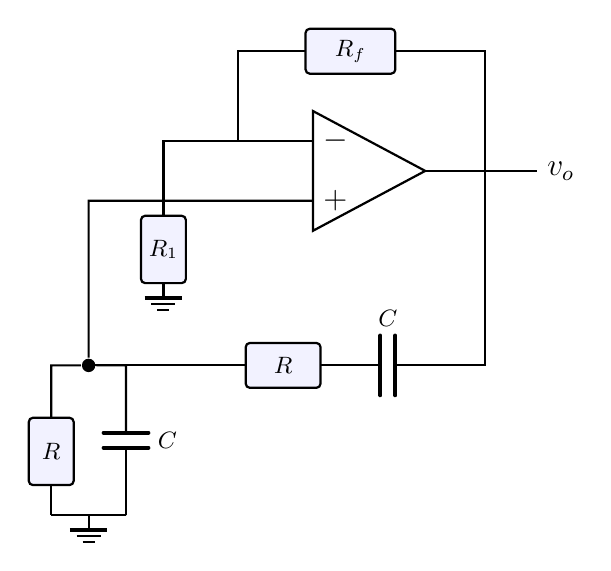
\begin{tikzpicture}[scale=0.95, transform shape]
  % Op-Amp
  \draw[thick, fill=white] (4.5, 2.0) -- (4.5, 3.6) -- (6.0, 2.8) -- cycle;
  \node at (4.8, 3.2) {\large $-$};
  \node at (4.8, 2.4) {\large $+$};
  \draw[thick] (6.0, 2.8) -- (7.5, 2.8) node[right] {\large $v_o$};

  % Inverting Feedback Branch (Rf and R1)
  \draw[thick] (4.5, 3.2) -- (3.5, 3.2) -- (3.5, 4.4) -- (4.4, 4.4);
  \draw[thick, fill=blue!5, rounded corners=1.5pt] (4.4, 4.1) rectangle (5.6, 4.7) node[midway] {\small $R_f$};
  \draw[thick] (5.6, 4.4) -- (6.8, 4.4) -- (6.8, 2.8);

  \draw[thick] (3.5, 3.2) -- (2.5, 3.2) -- (2.5, 2.2);
  \draw[thick, fill=blue!5, rounded corners=1.5pt] (2.2, 1.3) rectangle (2.8, 2.2) node[midway] {\small $R_1$};
  \draw[thick] (2.5, 1.3) -- (2.5, 1.1);
  \draw[line width=1.2pt] (2.25, 1.1) -- (2.75, 1.1);
  \draw[line width=1.0pt] (2.34, 1.02) -- (2.66, 1.02);
  \draw[line width=0.8pt] (2.42, 0.94) -- (2.58, 0.94);

  % Non-Inverting Feedback Lead-Lag Network
  \draw[thick] (6.8, 2.8) -- (6.8, 0.2) -- (5.6, 0.2);
  \draw[line width=1.4pt, line cap=round] (5.6, -0.2) -- (5.6, 0.6);
  \draw[line width=1.4pt, line cap=round] (5.4, -0.2) -- (5.4, 0.6);
  \node[above] at (5.5, 0.6) {\small $C$};
  \draw[thick] (5.4, 0.2) -- (4.6, 0.2);
  \draw[thick, fill=blue!5, rounded corners=1.5pt] (3.6, -0.1) rectangle (4.6, 0.5) node[midway] {\small $R$};
  \draw[thick] (3.6, 0.2) -- (1.5, 0.2) node[circle, fill, inner sep=1.8pt] (vfb) {};

  % Connection to Non-Inverting Input
  \draw[thick] (vfb) -- (1.5, 2.4) -- (4.5, 2.4);

  % Parallel R and C branch to ground
  \draw[thick] (vfb) -- (1.0, 0.2) -- (1.0, -0.5);
  \draw[thick, fill=blue!5, rounded corners=1.5pt] (0.7, -1.4) rectangle (1.3, -0.5) node[midway] {\small $R$};
  \draw[thick] (1.0, -1.4) -- (1.0, -1.8);

  \draw[thick] (vfb) -- (2.0, 0.2) -- (2.0, -0.7);
  \draw[line width=1.4pt, line cap=round] (1.7, -0.7) -- (2.3, -0.7);
  \draw[line width=1.4pt, line cap=round] (1.7, -0.9) -- (2.3, -0.9);
  \node[right] at (2.3, -0.8) {\small $C$};
  \draw[thick] (2.0, -0.9) -- (2.0, -1.8);

  \draw[thick] (1.0, -1.8) -- (2.0, -1.8) -- (1.5, -1.8) -- (1.5, -2.0);
  \draw[line width=1.2pt] (1.25, -2.0) -- (1.75, -2.0);
  \draw[line width=1.0pt] (1.34, -2.08) -- (1.66, -2.08);
  \draw[line width=0.8pt] (1.42, -2.16) -- (1.58, -2.16);
\end{tikzpicture}
\end{schematicbox}

\paragraph{Derivation of Resonant Frequency and Gain Requirement:}
The transfer function of the lead-lag feedback network $\beta(s) = \frac{v_f(s)}{v_o(s)}$ is:
\[
\beta(s) = \frac{Z_p}{Z_s + Z_p} = \frac{\frac{R}{1+sRC}}{\left(R + \frac{1}{sRC}\right) + \frac{R}{1+sRC}} = \frac{sRC}{(sRC)^2 + 3sRC + 1}
\]
Substituting $s = j\omega$:
\[
\beta(j\omega) = \frac{j\omega RC}{(1 - \omega^2 R^2 C^2) + 3j\omega RC}
\]
\begin{enumerate}[leftmargin=1.5em]
  \item \textbf{Oscillation Frequency ($f_0$):} For zero phase shift ($\angle \beta = 0^\circ$), the imaginary term in the bracket must vanish:
  \[
  1 - \omega_0^2 R^2 C^2 = 0 \implies \omega_0 = \frac{1}{RC} \implies \mathbf{f_0 = \frac{1}{2\pi RC}}
  \]
  \item \textbf{Attenuation at Resonance:}
  \[
  \beta(j\omega_0) = \frac{j}{3j} = \frac{1}{3}
  \]
  \item \textbf{Barkhausen Gain Requirement ($|A_v \beta| \ge 1$):}
  \[
  A_v = 1 + \frac{R_f}{R_1} \ge \frac{1}{\beta} = 3 \implies \mathbf{R_f \ge 2 R_1}
  \]
\end{enumerate}

\begin{answerbox}
$$\mathbf{f_0 = \frac{1}{2\pi RC}, \qquad R_f \ge 2 R_1 \quad (|A_v| \ge 3)}$$
\end{answerbox}

\vspace{0.6cm}

% =========================================================================
% QUESTION 6
% =========================================================================
\subsection{Question 6: Base-Current-Compensated Current Mirror [5 + 2 = 7 Marks]}
\begin{questionbox}{Problem Statement (2083 Baishakh, Q6)}
Explain how a base current compensation circuit reduces the difference between $I_O$ and $I_{\text{REF}}$ in a simple current mirror circuit.
\end{questionbox}

\paragraph{1. Circuit Description \& Role of Compensating Transistor $Q_3$:}
In a standard two-transistor current mirror, the reference branch must supply the base currents of both $Q_1$ and $Q_2$, introducing a relative error of $\approx 2/\beta$. A 3-transistor compensated current mirror inserts an emitter-follower transistor $Q_3$ to buffer the base currents.

\begin{schematicbox}{Base-Current-Compensated BJT Current Mirror Circuit}
\centering
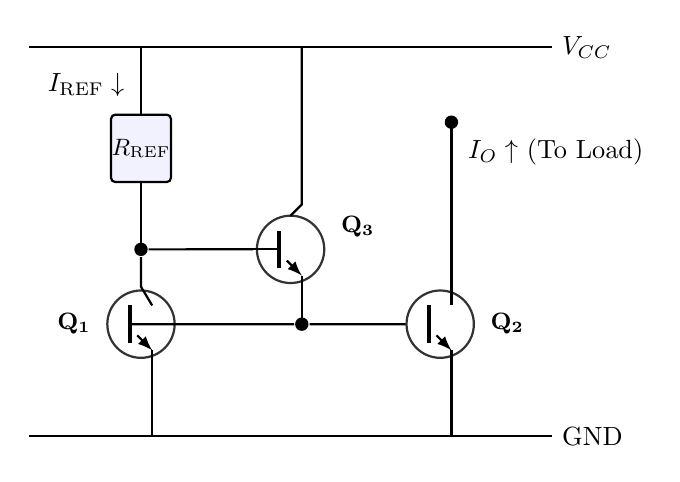
\begin{tikzpicture}[scale=0.95, transform shape]
  % Rails
  \draw[thick] (0, 5.2) -- (7.0, 5.2) node[right] {$V_{CC}$};
  \draw[thick] (0, 0) -- (7.0, 0) node[right] {GND};

  % R_REF
  \draw[thick] (1.5, 5.2) -- (1.5, 4.3);
  \draw[thick, fill=blue!5, rounded corners=1.5pt] (1.1, 3.4) rectangle (1.9, 4.3) node[midway] {\small $R_{\text{REF}}$};
  \draw[thick] (1.5, 3.4) -- (1.5, 2.5) node[circle, fill, inner sep=1.8pt] (n1) {};
  \node[left=0.1cm] at (1.5, 4.7) {$I_{\text{REF}} \downarrow$};

  % Transistor Q1 (NPN)
  \draw[thick] (n1) -- (1.5, 2.0);
  \draw[draw=black!80, fill=white, thick] (1.5, 1.5) circle (0.45cm);
  \draw[line width=1.4pt] (1.35, 1.25) -- (1.35, 1.75);
  \draw[thick] (1.5, 2.0) -- (1.65, 1.75); % Collector
  \draw[thick, ->, >=latex] (1.45, 1.35) -- (1.65, 1.15); % Emitter
  \draw[thick] (1.65, 1.15) -- (1.65, 0); % To GND
  \node[left=0.15cm] at (1.1, 1.5) {\small $\mathbf{Q_1}$};

  % Helper Transistor Q3 (NPN)
  \draw[thick] (n1) -- (3.0, 2.5); % Collector of Q1 to Base of Q3
  \draw[draw=black!80, fill=white, thick] (3.5, 2.5) circle (0.45cm);
  \draw[line width=1.4pt] (3.35, 2.25) -- (3.35, 2.75); % Base
  \draw[thick] (3.0, 2.5) -- (3.35, 2.5);
  \draw[thick] (3.5, 2.95) -- (3.65, 3.1) -- (3.65, 5.2); % Q3 Collector to VCC
  \draw[thick, ->, >=latex] (3.45, 2.35) -- (3.65, 2.15); % Q3 Emitter
  \draw[thick] (3.65, 2.15) -- (3.65, 1.5) node[circle, fill, inner sep=1.8pt] (n_bases) {};
  \node[right=0.15cm] at (3.9, 2.8) {\small $\mathbf{Q_3}$};

  % Connect Q3 emitter to bases of Q1 and Q2
  \draw[thick] (n_bases) -- (1.35, 1.5);
  \draw[thick] (n_bases) -- (5.35, 1.5);

  % Transistor Q2 (NPN)
  \draw[draw=black!80, fill=white, thick] (5.5, 1.5) circle (0.45cm);
  \draw[line width=1.4pt] (5.35, 1.25) -- (5.35, 1.75);
  \draw[thick, ->, >=latex] (5.45, 1.35) -- (5.65, 1.15); % Emitter
  \draw[thick] (5.65, 1.15) -- (5.65, 0); % To GND
  \draw[thick] (5.65, 1.75) -- (5.65, 4.2) node[circle, fill, inner sep=1.8pt] {};
  \node[right=0.1cm] at (5.65, 3.8) {$I_O \uparrow$ (To Load)};
  \node[right=0.15cm] at (5.9, 1.5) {\small $\mathbf{Q_2}$};
\end{tikzpicture}
\end{schematicbox}

\paragraph{2. Mathematical Derivation of Output Current $I_O$:}
\begin{enumerate}[leftmargin=1.5em]
  \item Assuming matched transistors ($I_{C1} = I_{C2} = I_O$ and $I_{B1} = I_{B2} = I_B = \frac{I_O}{\beta}$):
  \[
  I_{E3} = I_{B1} + I_{B2} = 2 I_B = \frac{2 I_O}{\beta}
  \]
  \item Transistor $Q_3$ base current is reduced by a factor of $(1+\beta)$:
  \[
  I_{B3} = \frac{I_{E3}}{1+\beta} = \frac{2 I_O}{\beta(1+\beta)} \approx \frac{2 I_O}{\beta^2}
  \]
  \item Applying KCL at the reference collector node:
  \[
  I_{\text{REF}} = I_{C1} + I_{B3} = I_O + \frac{2 I_O}{\beta(\beta + 1)} = I_O \left[1 + \frac{2}{\beta^2 + \beta}\right]
  \]
  \[
  \mathbf{I_O = \frac{I_{\text{REF}}}{1 + \frac{2}{\beta^2 + \beta}} \approx I_{\text{REF}} \left(1 - \frac{2}{\beta^2}\right)}
  \]
\end{enumerate}

\paragraph{3. Error Comparison:}
\begin{itemize}[leftmargin=1.5em]
  \item Simple 2-BJT Mirror Error: $\frac{|I_{\text{REF}} - I_O|}{I_{\text{REF}}} \approx \frac{2}{\beta} = 2.0\%$ (for $\beta = 100$).
  \item Base-Compensated Mirror Error: $\frac{|I_{\text{REF}} - I_O|}{I_{\text{REF}}} \approx \frac{2}{\beta^2} = 0.02\%$ (a **100-fold accuracy improvement**).
\end{itemize}

\begin{answerbox}
$$\mathbf{I_O = \frac{I_{\text{REF}}}{1 + \frac{2}{\beta^2 + \beta}} \approx I_{\text{REF}} \left(1 - \frac{2}{\beta^2}\right) \implies \text{Error reduced from } O(1/\beta) \text{ to } O(1/\beta^2)}$$
\end{answerbox}

\vspace{0.6cm}

% =========================================================================
% QUESTION 7
% =========================================================================
\subsection{Question 7: Class B Power Amplifier Calculations [6 Marks]}
\begin{questionbox}{Problem Statement (2083 Baishakh, Q7)}
For a class B amplifier providing a $20\text{ V peak}$ signal to a $16\ \Omega$ load (speaker) and a power supply of $V_{CC} = 30\text{ V}$, determine the input power, output power, and circuit efficiency.
\end{questionbox}

\begin{enumerate}[leftmargin=1.5em]
  \item \textbf{Peak Output Voltage ($V_p$):}
  \[
  V_p = \mathbf{20.0\text{ V}}
  \]
  \item \textbf{AC Output Signal Power ($P_{o(\text{ac})}$):}
  \[
  P_{o(\text{ac})} = \frac{V_p^2}{2 R_L} = \frac{(20\text{ V})^2}{2 \times 16\ \Omega} = \frac{400}{32} = \mathbf{12.5\text{ W}}
  \]
  \item \textbf{Average DC Supply Current ($I_{\text{dc}}$):}
  For a complementary Class B push-pull amplifier, each transistor conducts over half a cycle:
  \[
  I_{\text{dc}} = \frac{2}{\pi} I_p = \frac{2}{\pi} \left(\frac{V_p}{R_L}\right) = \frac{2}{\pi} \left(\frac{20\text{ V}}{16\ \Omega}\right) = \frac{40}{16\pi} = \frac{2.5}{\pi} \approx \mathbf{0.7958\text{ A}}
  \]
  \item \textbf{DC Input Power ($P_{i(\text{dc})}$):}
  \[
  P_{i(\text{dc})} = V_{CC} I_{\text{dc}} = 30\text{ V} \times 0.7958\text{ A} = \frac{75}{\pi} \approx \mathbf{23.873\text{ W}}
  \]
  \item \textbf{Circuit Conversion Efficiency ($\eta$):}
  \[
  \mathbf{\eta = \frac{P_{o(\text{ac})}}{P_{i(\text{dc})}} \times 100\% = \frac{12.5\text{ W}}{23.873\text{ W}} \times 100\% = \frac{\pi}{4} \left(\frac{V_p}{V_{CC}}\right) \times 100\% = \frac{\pi}{4} \left(\frac{20\text{ V}}{30\text{ V}}\right) \times 100\% = \mathbf{52.36\%}}
  \]
  \item \textbf{Total Transistor Power Dissipation ($P_{d(\text{total})}$):}
  \[
  P_{d(\text{total})} = P_{i(\text{dc})} - P_{o(\text{ac})} = 23.873\text{ W} - 12.5\text{ W} = \mathbf{11.373\text{ W}} \quad (5.687\text{ W per transistor})
  \]
\end{enumerate}

\begin{answerbox}
$$\mathbf{P_{o(\text{ac})} = 12.50\text{ W}, \qquad P_{i(\text{dc})} = 23.87\text{ W}, \qquad \eta = 52.36\%}$$
\end{answerbox}

\vspace{0.6cm}

% =========================================================================
% QUESTION 8
% =========================================================================
\subsection{Question 8: Transformer-Coupled Class A Power Amplifier [7 Marks]}
\begin{questionbox}{Problem Statement (2083 Baishakh, Q8)}
Draw the circuit diagram and the characteristic curve of a transformer-coupled class A amplifier and derive its general and maximum efficiency.
\end{questionbox}

\paragraph{1. Circuit Operation:}
A step-down output transformer matches the high collector output impedance to a low-impedance loudspeaker ($R_L$). The reflected AC load resistance seen by the primary is $R_L' = \left(\frac{N_1}{N_2}\right)^2 R_L$.

\begin{schematicbox}{Transformer-Coupled Class A Amplifier Circuit \& Dynamic AC/DC Load Line Curves}
\centering
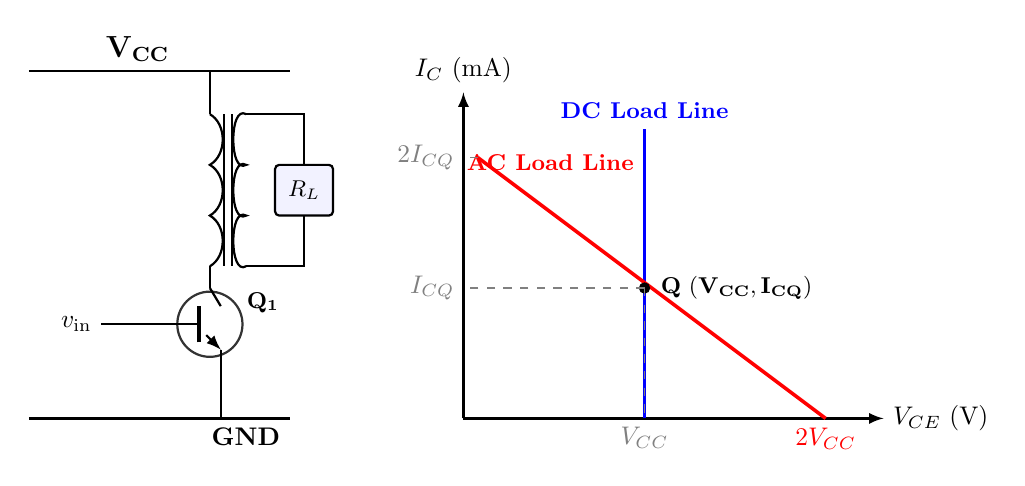
\begin{tikzpicture}[scale=0.92, transform shape]
  % Circuit (Left)
  \draw[thick] (0, 4.8) -- (3.6, 4.8);
  \node[above] at (1.5, 4.8) {\large $\mathbf{V_{CC}}$};
  \draw[thick] (0, 0) -- (3.6, 0) node[below left] {\textbf{GND}};

  % Transformer Primary
  \draw[thick] (2.5, 4.8) -- (2.5, 4.2);
  \draw[thick] (2.5, 4.2) to[out=-30, in=30] (2.5, 3.5) to[out=-30, in=30] (2.5, 2.8) to[out=-30, in=30] (2.5, 2.1);
  \draw[thick] (2.5, 2.1) -- (2.5, 1.8);

  % Core
  \draw[thick] (2.7, 4.2) -- (2.7, 2.1);
  \draw[thick] (2.8, 4.2) -- (2.8, 2.1);

  % Secondary
  \draw[thick] (3.0, 4.2) to[out=150, in=-150] (3.0, 3.5) to[out=150, in=-150] (3.0, 2.8) to[out=150, in=-150] (3.0, 2.1);
  \draw[thick] (3.0, 4.2) -- (3.8, 4.2) -- (3.8, 3.5);
  \draw[thick, fill=blue!5, rounded corners=1.5pt] (3.4, 2.8) rectangle (4.2, 3.5) node[midway] {\small $R_L$};
  \draw[thick] (3.8, 2.8) -- (3.8, 2.1) -- (3.0, 2.1);

  % Transistor Q1 (NPN)
  \draw[draw=black!80, fill=white, thick] (2.5, 1.3) circle (0.45cm);
  \draw[line width=1.4pt] (2.35, 1.05) -- (2.35, 1.55);
  \draw[thick] (1.0, 1.3) node[left] {$v_{\text{in}}$} -- (2.35, 1.3);
  \draw[thick] (2.5, 1.8) -- (2.65, 1.55);
  \draw[thick, ->, >=latex] (2.45, 1.15) -- (2.65, 0.95);
  \draw[thick] (2.65, 0.95) -- (2.65, 0);
  \node[above right=0.05cm] at (2.85, 1.3) {\small $\mathbf{Q_1}$};

  % Characteristic AC/DC Load Line (Right)
  \draw[thick, ->, >=latex] (6.0, 0) -- (11.8, 0) node[right] {$V_{CE}\ (\text{V})$};
  \draw[thick, ->, >=latex] (6.0, 0) -- (6.0, 4.5) node[above] {$I_C\ (\text{mA})$};

  % DC Load line (Vertical line at VCC because R_dc approx 0)
  \draw[line width=1.2pt, blue] (8.5, 0) -- (8.5, 4.0) node[above] {\small\textbf{DC Load Line}};

  % AC Load line (Slope = -1/RL')
  \draw[line width=1.3pt, red] (6.2, 3.6) -- (11.0, 0) node[below] {$2V_{CC}$};
  \node[above=0.1cm, red] at (7.2, 3.2) {\small\textbf{AC Load Line}};

  % Q point
  \draw[fill=black] (8.5, 1.8) circle (2pt) node[right=0.1cm] {\small $\mathbf{Q\ (V_{CC}, I_{CQ})}$};
  \draw[dashed, gray] (8.5, 1.8) -- (6.0, 1.8) node[left] {$I_{CQ}$};
  \draw[dashed, gray] (6.2, 3.6) -- (6.0, 3.6) node[left] {$2I_{CQ}$};
  \draw[dashed, gray] (8.5, 1.8) -- (8.5, 0) node[below] {$V_{CC}$};
\end{tikzpicture}
\end{schematicbox}

\paragraph{2. Efficiency Derivation:}
\begin{enumerate}[leftmargin=1.5em]
  \item \textbf{DC Input Power:} At quiescent bias $V_{CEQ} = V_{CC}$ (since primary DC winding resistance is $\approx 0\ \Omega$):
  \[
  P_{i(\text{dc})} = V_{CC} I_{CQ}
  \]
  \item \textbf{AC Output Power:}
  \[
  P_{o(\text{ac})} = \frac{V_p I_p}{2} = \frac{(V_{\max} - V_{\min})(I_{\max} - I_{\min})}{8}
  \]
  \item \textbf{General Efficiency ($\eta$):}
  \[
  \mathbf{\eta = \frac{P_{o(\text{ac})}}{P_{i(\text{dc})}} = \frac{\frac{V_p I_p}{2}}{V_{CC} I_{CQ}} = \frac{1}{2} \left(\frac{V_p}{V_{CC}}\right) \left(\frac{I_p}{I_{CQ}}\right) \times 100\%}
  \]
  \item \textbf{Maximum Efficiency ($\eta_{\max}$):} For maximum symmetrical undistorted output swing, $V_p = V_{CC}$ (voltage swings between $0\text{ V}$ and $2V_{CC}$) and $I_p = I_{CQ}$:
  \[
  \mathbf{\eta_{\max} = \frac{1}{2} (1)(1) \times 100\% = 50.0\%}
  \]
\end{enumerate}

\begin{answerbox}
$$\mathbf{\eta = \frac{1}{2} \left(\frac{V_p}{V_{CC}}\right) \left(\frac{I_p}{I_{CQ}}\right) \times 100\%, \qquad \eta_{\max} = 50.0\%}$$
\end{answerbox}

\vspace{0.6cm}

% =========================================================================
% QUESTION 9
% =========================================================================
\subsection{Question 9: Stability Factor of Discrete Series Voltage Regulator [4 Marks]}
\begin{questionbox}{Problem Statement (2083 Baishakh, Q9)}
Derive the expression for stability factor of a discrete-transistor series regulator.
\end{questionbox}

\paragraph{1. Circuit Model \& Voltage Stability Factor Definition:}
The Voltage Stability Factor ($S_V$) defines the line regulation capability of the series voltage regulator:
\[
S_V = \left.\frac{\Delta V_o}{\Delta V_{\text{in}}}\right|_{R_L = \text{constant}}
\]

\begin{schematicbox}{Discrete Transistor Series Voltage Regulator Small-Signal Circuit}
\centering
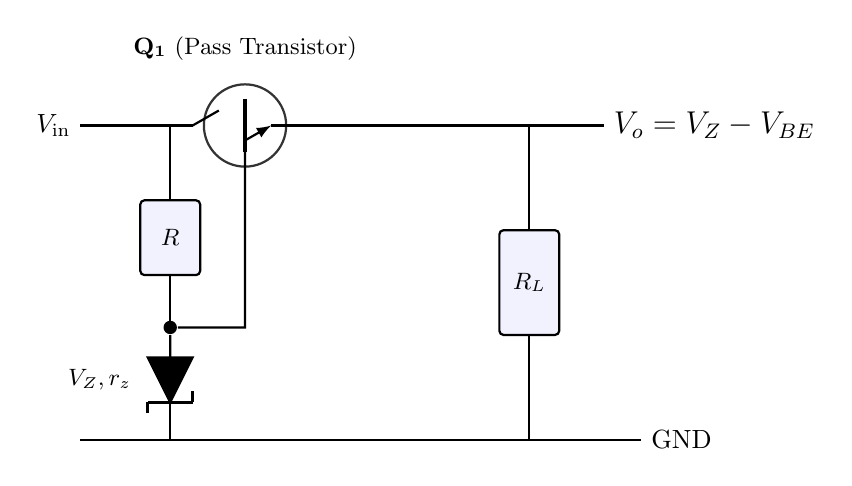
\begin{tikzpicture}[scale=0.95, transform shape]
  % Rails
  \draw[thick] (0, 4.2) node[left] {$V_{\text{in}}$} -- (1.5, 4.2);
  \draw[thick] (0, 0) -- (7.5, 0) node[right] {GND};

  % Pass Transistor Q1 (NPN)
  \draw[draw=black!80, fill=white, thick] (2.2, 4.2) circle (0.55cm);
  \draw[line width=1.6pt] (2.2, 3.85) -- (2.2, 4.55); % Base
  \draw[thick] (1.5, 4.2) -- (1.85, 4.4); % Collector
  \draw[thick, ->, >=latex] (2.2, 4.0) -- (2.55, 4.2); % Emitter
  \draw[thick] (2.55, 4.2) -- (7.0, 4.2) node[right] {\large $V_o = V_Z - V_{BE}$};
  \node[above=0.2cm] at (2.2, 4.75) {\small $\mathbf{Q_1}$ (Pass Transistor)};

  % Base bias branch
  \draw[thick] (1.2, 4.2) -- (1.2, 3.2);
  \draw[thick, fill=blue!5, rounded corners=1.5pt] (0.8, 2.2) rectangle (1.6, 3.2) node[midway] {\small $R$};
  \draw[thick] (1.2, 2.2) -- (1.2, 1.5) node[circle, fill, inner sep=1.8pt] (nb) {};
  \draw[thick] (nb) -- (2.2, 1.5) -- (2.2, 3.85); % Base connection

  % Zener Diode
  \draw[thick] (nb) -- (1.2, 1.1);
  \draw[thick, fill=black] (0.9, 1.1) -- (1.5, 1.1) -- (1.2, 0.5) -- cycle;
  \draw[line width=1.2pt] (0.9, 0.5) -- (1.5, 0.5);
  \draw[line width=1.2pt] (0.9, 0.5) -- (0.9, 0.35);
  \draw[line width=1.2pt] (1.5, 0.5) -- (1.5, 0.65);
  \node[left=0.1cm] at (0.9, 0.8) {\small $V_Z, r_z$};
  \draw[thick] (1.2, 0.5) -- (1.2, 0);

  % Load Resistor
  \draw[thick] (6.0, 4.2) -- (6.0, 2.8);
  \draw[thick, fill=blue!5, rounded corners=1.5pt] (5.6, 1.4) rectangle (6.4, 2.8) node[midway] {\small $R_L$};
  \draw[thick] (6.0, 1.4) -- (6.0, 0);
\end{tikzpicture}
\end{schematicbox}

\paragraph{2. Derivation of Stability Factor $S_V$:}
\begin{enumerate}[leftmargin=1.5em]
  \item The Zener diode has dynamic internal resistance $r_z$. A change in input voltage $\Delta V_{\text{in}}$ produces a change in Zener voltage $\Delta V_Z$ through the voltage divider formed by $R$ and $r_z$:
  \[
  \Delta V_Z = \Delta V_{\text{in}} \left(\frac{r_z}{R + r_z}\right)
  \]
  \item The output voltage follows the base voltage via the emitter-follower pass transistor $Q_1$:
  \[
  V_o = V_Z - V_{BE} \implies \Delta V_o = \Delta V_Z - \Delta V_{BE}
  \]
  \item Since the base-emitter voltage drop $V_{BE} \approx 0.7\text{ V}$ remains virtually constant ($\Delta V_{BE} \approx 0$):
  \[
  \Delta V_o \approx \Delta V_Z = \Delta V_{\text{in}} \left(\frac{r_z}{R + r_z}\right)
  \]
  \item Therefore, the voltage stability factor is:
  \[
  \mathbf{S_V = \frac{\Delta V_o}{\Delta V_{\text{in}}} = \frac{r_z}{R + r_z}}
  \]
\end{enumerate}
For good line regulation, $r_z \ll R$, which ensures $S_V \ll 1$ (typically $S_V \approx 0.01 - 0.05$).

\begin{answerbox}
$$\mathbf{S_V = \frac{\Delta V_o}{\Delta V_{\text{in}}} = \frac{r_z}{R + r_z} \approx \frac{r_z}{R} \ll 1}$$
\end{answerbox}

\vspace{0.6cm}

% =========================================================================
% QUESTION 10
% =========================================================================
\subsection{Question 10: LM317 Variable DC Voltage Regulator Design (3V - 15V) [4 Marks]}
\begin{questionbox}{Problem Statement (2083 Baishakh, Q10)}
Design a variable DC voltage regulator using the LM317 to output (3-15) volts.
\end{questionbox}

The LM317 maintains a precision internal reference voltage of $V_{\text{ref}} = 1.25\text{ V}$ between its Output and Adjust terminals:
\[
V_{\text{out}} = V_{\text{ref}} \left(1 + \frac{R_2}{R_1}\right) + I_{\text{adj}} R_2 \approx 1.25\text{ V} \left(1 + \frac{R_2}{R_1}\right) \quad (\text{since } I_{\text{adj}} \approx 50\ \mu\text{A} \text{ is negligible})
\]

\begin{schematicbox}{LM317 Adjustable Linear Voltage Regulator Circuit}
\centering
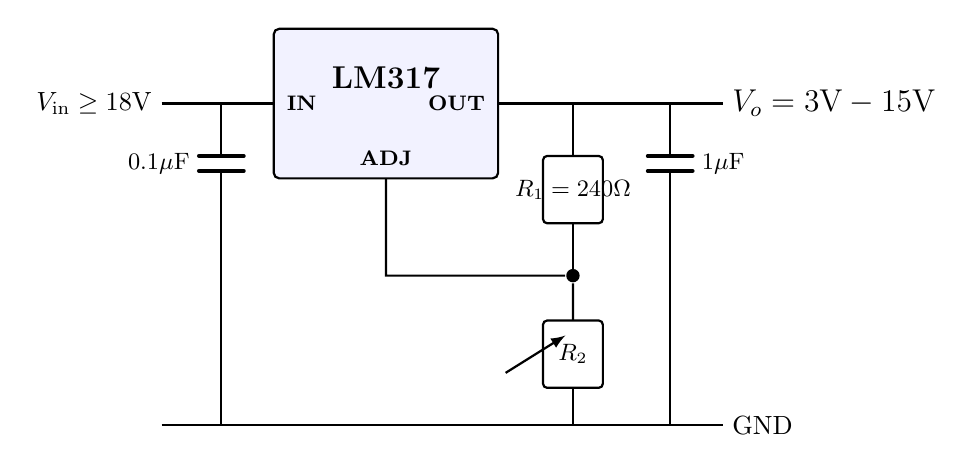
\begin{tikzpicture}[scale=0.95, transform shape]
  % Input
  \draw[thick] (0, 2.5) node[left] {$V_{\text{in}} \ge 18\text{V}$} -- (1.5, 2.5);
  % Cin
  \draw[thick] (0.8, 2.5) -- (0.8, 1.8);
  \draw[line width=1.4pt, line cap=round] (0.5, 1.8) -- (1.1, 1.8);
  \draw[line width=1.4pt, line cap=round] (0.5, 1.6) -- (1.1, 1.6);
  \node[left] at (0.5, 1.7) {\small $0.1\mu\text{F}$};
  \draw[thick] (0.8, 1.6) -- (0.8, 0);

  % LM317 IC Box
  \draw[thick, fill=blue!5, rounded corners=2pt] (1.5, 1.5) rectangle (4.5, 3.5);
  \node at (3.0, 2.85) {\large\textbf{LM317}};
  \node[right] at (1.55, 2.5) {\footnotesize \textbf{IN}};
  \node[left] at (4.45, 2.5) {\footnotesize \textbf{OUT}};
  \node[above] at (3.0, 1.55) {\footnotesize \textbf{ADJ}};

  % Output rail
  \draw[thick] (4.5, 2.5) -- (7.5, 2.5) node[right] {\large $V_o = 3\text{V}-15\text{V}$};

  % R1 Resistor
  \draw[thick] (5.5, 2.5) -- (5.5, 1.8);
  \draw[thick, fill=white, rounded corners=1.5pt] (5.1, 0.9) rectangle (5.9, 1.8) node[midway] {\small $R_1=240\Omega$};
  \draw[thick] (5.5, 0.9) -- (5.5, 0.2) node[circle, fill, inner sep=1.8pt] (n_adj) {};
  \draw[thick] (n_adj) -- (3.0, 0.2) -- (3.0, 1.5);

  % R2 Potentiometer
  \draw[thick] (n_adj) -- (5.5, -0.4);
  \draw[thick, fill=white, rounded corners=1.5pt] (5.1, -1.3) rectangle (5.9, -0.4) node[midway] {\small $R_2$};
  \draw[thick, ->, >=latex] (4.6, -1.1) -- (5.4, -0.6); % Arrow for pot
  \draw[thick] (5.5, -1.3) -- (5.5, -1.8);

  % Cout
  \draw[thick] (6.8, 2.5) -- (6.8, 1.8);
  \draw[line width=1.4pt, line cap=round] (6.5, 1.8) -- (7.1, 1.8);
  \draw[line width=1.4pt, line cap=round] (6.5, 1.6) -- (7.1, 1.6);
  \node[right] at (7.1, 1.7) {\small $1\mu\text{F}$};
  \draw[thick] (6.8, 1.6) -- (6.8, -1.8);

  % Ground rail
  \draw[thick] (0, -1.8) -- (7.5, -1.8) node[right] {GND};
  \draw[thick] (0.8, 0) -- (0.8, -1.8);
\end{tikzpicture}
\end{schematicbox}

\paragraph{Component Value Calculations:}
\begin{enumerate}[leftmargin=1.5em]
  \item Standard program resistor selection: $R_1 = \mathbf{240\ \Omega}$ (satisfies $I_L \ge 5\text{ mA}$ minimum load requirement).
  \item For minimum output $V_{\text{out}(\min)} = 3.0\text{ V}$:
  \[
  3.0 = 1.25 \left(1 + \frac{R_{2(\min)}}{240}\right) \implies 1 + \frac{R_{2(\min)}}{240} = 2.4 \implies R_{2(\min)} = 1.4 \times 240 = \mathbf{336\ \Omega}
  \]
  \item For maximum output $V_{\text{out}(\max)} = 15.0\text{ V}$:
  \[
  15.0 = 1.25 \left(1 + \frac{R_{2(\max)}}{240}\right) \implies 1 + \frac{R_{2(\max)}}{240} = 12.0 \implies R_{2(\max)} = 11 \times 240 = \mathbf{2640\ \Omega} = \mathbf{2.64\text{ k}\Omega}
  \]
\end{enumerate}
\textbf{Practical Realization:} Use a fixed resistor $R_{2A} = 330\ \Omega$ in series with a $\mathbf{2.5\text{ k}\Omega}$ linear potentiometer ($R_2 = 330\ \Omega \text{ to } 2.83\text{ k}\Omega$). Input DC voltage requirement: $V_{\text{in}} \ge V_{\text{out}(\max)} + 3\text{ V} = 18\text{ V DC}$.

\begin{answerbox}
$$\mathbf{R_1 = 240\ \Omega, \qquad R_2 = 336\ \Omega \text{ to } 2.64\text{ k}\Omega \quad (\text{Fixed } 330\ \Omega + 2.5\text{ k}\Omega \text{ Potentiometer}), \qquad V_{\text{in}} \ge 18\text{ V}}$$
\end{answerbox}

\chapter{2082 Bhadra Examination Solutions}

\section*{Examination Overview}
\begin{tabular}{@{}ll@{}}
\textbf{Level:} Bachelor in Engineering (BE) & \textbf{Full Marks:} 60 \\
\textbf{Programme:} BEI, BCT & \textbf{Pass Marks:} 24 \\
\textbf{Year / Part:} I / II & \textbf{Time:} 3 Hours \\
\textbf{Subject:} Electronic Devices \& Circuits (ENEX 151) & \textbf{Examination Type:} Regular (New Course) \\
\end{tabular}

\vspace{0.6cm}
\hrule
\vspace{0.6cm}

% =========================================================================
% QUESTION 1
% =========================================================================
\subsection{Question 1: $\beta$-Independent Voltage Divider Bias Design [1 + 5 = 6 Marks]}
\begin{questionbox}{Problem Statement (2082 Bhadra, Q1)}
What is the significance of $\beta$-independency in a voltage divider biasing circuit? Design a $\beta$-independent voltage divider bias circuit for the given parameters: $V_{CC} = 15\text{ V}, I_E = 1\text{ mA}$, and $\beta = 100$.
\end{questionbox}

\paragraph{Part (a): Significance of $\beta$-Independency [1 Mark]}
Transistor forward current gain $\beta$ ($h_{FE}$) exhibits wide manufacturing dispersions (typically ranging from 100 to 300 for the same transistor type) and strong temperature dependence ($+0.5\%/^\circ\text{C}$). A $\beta$-independent biasing circuit ensures that the quiescent operating point ($I_{CQ}, V_{CEQ}$) remains strictly invariant against device replacement and thermal drift, completely avoiding thermal runaway and waveform clipping.

\paragraph{Part (b): Step-by-Step Design [5 Marks]}
Design Specifications: $V_{CC} = 15\text{ V}, I_{E} \approx I_{CQ} = 1.0\text{ mA}, \beta = 100$, Silicon BJT ($V_{BE} = 0.7\text{ V}$).

\begin{enumerate}[leftmargin=1.5em]
  \item \textbf{Emitter Voltage Allocation ($V_E$):}
  To ensure excellent temperature stability without compromising dynamic output voltage swing, allocate 10\% of $V_{CC}$:
  \[
  V_E = 0.10 \times V_{CC} = 0.10 \times 15\text{ V} = \mathbf{1.5\text{ V}}
  \]
  \item \textbf{Calculation of $R_E$:}
  \[
  R_E = \frac{V_E}{I_E} = \frac{1.5\text{ V}}{1.0\text{ mA}} = \mathbf{1.5\text{ k}\Omega}
  \]
  \item \textbf{Collector Voltage Allocation ($V_C$):}
  For maximum symmetrical undistorted output voltage swing:
  \[
  V_{CEQ} = \frac{V_{CC} - V_E}{2} = \frac{15\text{ V} - 1.5\text{ V}}{2} = 6.75\text{ V}
  \]
  \[
  V_C = V_E + V_{CEQ} = 1.5\text{ V} + 6.75\text{ V} = 8.25\text{ V}
  \]
  \[
  R_C = \frac{V_{CC} - V_C}{I_C} = \frac{15\text{ V} - 8.25\text{ V}}{1.0\text{ mA}} = 6.75\text{ k}\Omega \quad (\text{Select standard value } R_C = \mathbf{6.8\text{ k}\Omega})
  \]
  \item \textbf{Base Voltage ($V_B$):}
  \[
  V_B = V_E + V_{BE} = 1.5\text{ V} + 0.7\text{ V} = \mathbf{2.2\text{ V}}
  \]
  \item \textbf{Voltage Divider Resistors ($R_1, R_2$) via Bleeder Current Rule ($I_{\text{bleed}} \ge 10 I_B$):}
  \[
  I_B = \frac{I_C}{\beta} = \frac{1.0\text{ mA}}{100} = 0.01\text{ mA} = 10\ \mu\text{A} \implies I_{\text{bleed}} = 10 \times I_B = 0.10\text{ mA}
  \]
  \[
  R_2 = \frac{V_B}{I_{\text{bleed}}} = \frac{2.2\text{ V}}{0.10\text{ mA}} = \mathbf{22\text{ k}\Omega} \quad (\text{Standard } 5\% \text{ resistor})
  \]
  \[
  R_1 = \frac{V_{CC} - V_B}{I_{\text{bleed}} + I_B} = \frac{15\text{ V} - 2.2\text{ V}}{0.10\text{ mA} + 0.01\text{ mA}} = \frac{12.8\text{ V}}{0.11\text{ mA}} = 116.36\text{ k}\Omega \quad (\text{Select standard } R_1 = \mathbf{120\text{ k}\Omega})
  \]
\end{enumerate}

\begin{schematicbox}{Designed Common Emitter Amplifier Circuit ($V_{CC} = 15\text{V}$)}
\centering
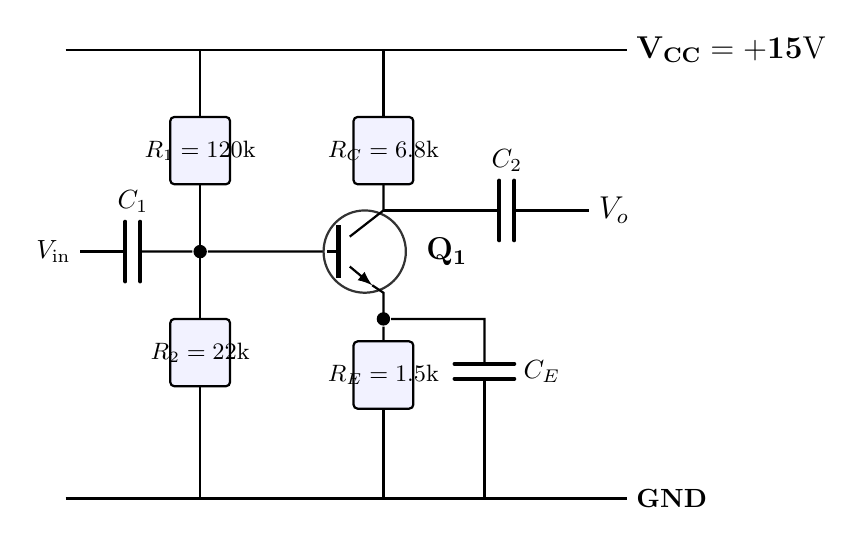
\begin{tikzpicture}[scale=0.95, transform shape]
  % Rails
  \draw[thick] (0, 5.2) -- (7.5, 5.2) node[right] {\large $\mathbf{V_{CC} = +15\text{V}}$};
  \draw[thick] (0, -0.8) -- (7.5, -0.8) node[right] {\textbf{GND}};

  % Divider R1 and R2
  \draw[thick] (1.8, 5.2) -- (1.8, 4.3);
  \draw[thick, fill=blue!5, rounded corners=1.5pt] (1.4, 3.4) rectangle (2.2, 4.3) node[midway] {\small $R_1=120\text{k}$};
  \draw[thick] (1.8, 3.4) -- (1.8, 2.5) node[circle, fill, inner sep=1.8pt] (vb) {};
  \draw[thick] (1.8, 2.5) -- (1.8, 1.6);
  \draw[thick, fill=blue!5, rounded corners=1.5pt] (1.4, 0.7) rectangle (2.2, 1.6) node[midway] {\small $R_2=22\text{k}$};
  \draw[thick] (1.8, 0.7) -- (1.8, -0.8);

  % Input coupling capacitor C1
  \draw[thick] (0.2, 2.5) node[left] {$V_{\text{in}}$} -- (0.8, 2.5);
  \draw[line width=1.4pt, line cap=round] (0.8, 2.1) -- (0.8, 2.9);
  \draw[line width=1.4pt, line cap=round] (1.0, 2.1) -- (1.0, 2.9);
  \node[above] at (0.9, 2.9) {$C_1$};
  \draw[thick] (1.0, 2.5) -- (vb);

  % Transistor Q1 (NPN)
  \draw[thick] (vb) -- (3.5, 2.5);
  \draw[draw=black!80, fill=white, thick] (4.0, 2.5) circle (0.55cm);
  \draw[line width=1.6pt] (3.65, 2.15) -- (3.65, 2.85); % Base
  \draw[thick] (3.5, 2.5) -- (3.65, 2.5);
  \draw[thick] (3.8, 2.7) -- (4.25, 3.05) -- (4.25, 3.4); % Collector
  \draw[thick, ->, >=latex] (3.8, 2.3) -- (4.1, 2.05); % Emitter
  \draw[thick] (4.1, 2.05) -- (4.25, 1.95) -- (4.25, 1.6) node[circle, fill, inner sep=1.8pt] (ve) {};
  \node[right=0.2cm] at (4.5, 2.5) {\large $\mathbf{Q_1}$};

  % Collector Resistor RC
  \draw[thick, fill=blue!5, rounded corners=1.5pt] (3.85, 3.4) rectangle (4.65, 4.3) node[midway] {\small $R_C=6.8\text{k}$};
  \draw[thick] (4.25, 4.3) -- (4.25, 5.2);

  % Emitter Resistor RE and Bypass CE
  \draw[thick] (ve) -- (4.25, 1.3);
  \draw[thick, fill=blue!5, rounded corners=1.5pt] (3.85, 0.4) rectangle (4.65, 1.3) node[midway] {\small $R_E=1.5\text{k}$};
  \draw[thick] (4.25, 0.4) -- (4.25, -0.8);

  % Bypass Capacitor CE
  \draw[thick] (ve) -- (5.6, 1.6) -- (5.6, 1.0);
  \draw[line width=1.4pt, line cap=round] (5.2, 1.0) -- (6.0, 1.0);
  \draw[line width=1.4pt, line cap=round] (5.2, 0.8) -- (6.0, 0.8);
  \node[right] at (6.0, 0.9) {$C_E$};
  \draw[thick] (5.6, 0.8) -- (5.6, -0.8);

  % Output coupling capacitor C2
  \draw[thick] (4.25, 3.05) -- (5.8, 3.05);
  \draw[line width=1.4pt, line cap=round] (5.8, 2.65) -- (5.8, 3.45);
  \draw[line width=1.4pt, line cap=round] (6.0, 2.65) -- (6.0, 3.45);
  \node[above] at (5.9, 3.45) {$C_2$};
  \draw[thick] (6.0, 3.05) -- (7.0, 3.05) node[right] {\large $V_o$};
\end{tikzpicture}
\end{schematicbox}

\begin{answerbox}
$$\mathbf{R_1 = 120\text{ k}\Omega, \quad R_2 = 22\text{ k}\Omega, \quad R_C = 6.8\text{ k}\Omega, \quad R_E = 1.5\text{ k}\Omega}$$
\end{answerbox}

\vspace{0.6cm}

% =========================================================================
% QUESTION 2
% =========================================================================
\subsection{Question 2: Role of Coupling Capacitors \& CE Small Signal Parameters [2 + 5 = 7 Marks]}
\begin{questionbox}{Problem Statement (2082 Bhadra, Q2)}
Explain the role of coupling capacitors in amplifier circuits. Draw the small signal equivalent circuit of a common emitter amplifier circuit and find its input impedance, output impedance and voltage gain.
\end{questionbox}

\paragraph{Part (a): Role of Coupling Capacitors ($C_{\text{in}}, C_{\text{out}}$) [2 Marks]}
Coupling capacitors block DC operating voltages from entering the external AC signal source or load resistor, preventing quiescent operating point shifts while presenting a negligible impedance path ($X_C = \frac{1}{2\pi f C} \approx 0$) for signal frequencies.

\paragraph{Part (b): Common Emitter Parameter Derivations [5 Marks]}
\begin{schematicbox}{Small-Signal Model of Common Emitter BJT Amplifier}
\centering
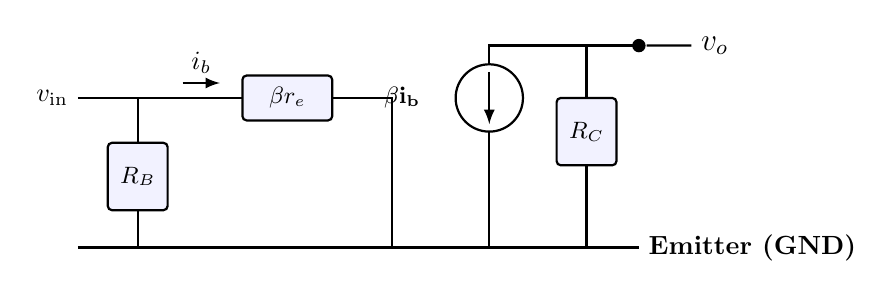
\begin{tikzpicture}[scale=0.95, transform shape]
  % Input
  \draw[thick] (0, 2.0) node[left] {$v_{\text{in}}$} -- (1.2, 2.0);
  % R_B (R1 || R2)
  \draw[thick] (0.8, 2.0) -- (0.8, 1.4);
  \draw[thick, fill=blue!5, rounded corners=1.5pt] (0.4, 0.5) rectangle (1.2, 1.4) node[midway] {\small $R_B$};
  \draw[thick] (0.8, 0.5) -- (0.8, 0);

  % Base resistance beta * re
  \draw[thick] (1.2, 2.0) -- (2.2, 2.0);
  \draw[thick, fill=blue!5, rounded corners=1.5pt] (2.2, 1.7) rectangle (3.4, 2.3) node[midway] {\small $\beta r_e$};
  \draw[thick] (3.4, 2.0) -- (4.2, 2.0) -- (4.2, 0);
  \draw[thick, ->, >=latex] (1.4, 2.2) -- (1.9, 2.2) node[midway, above] {$i_b$};

  % Dependent current source beta * ib
  \draw[thick] (5.5, 2.0) circle (0.45cm);
  \draw[thick, ->, >=latex] (5.5, 2.35) -- (5.5, 1.65);
  \node[left=0.15cm] at (4.85, 2.0) {\small $\mathbf{\beta i_b}$};
  \draw[thick] (5.5, 1.55) -- (5.5, 0);
  \draw[thick] (5.5, 2.45) -- (5.5, 2.7) -- (7.5, 2.7) node[circle, fill, inner sep=1.8pt] (c_node) {};

  % Output Resistance RC
  \draw[thick] (6.8, 2.7) -- (6.8, 2.0);
  \draw[thick, fill=blue!5, rounded corners=1.5pt] (6.4, 1.1) rectangle (7.2, 2.0) node[midway] {\small $R_C$};
  \draw[thick] (6.8, 1.1) -- (6.8, 0);

  % Ground Rail
  \draw[thick] (0, 0) -- (7.5, 0) node[right] {\textbf{Emitter (GND)}};

  % Output terminal
  \draw[thick] (c_node) -- (8.2, 2.7) node[right] {\large $v_o$};
\end{tikzpicture}
\end{schematicbox}

\begin{enumerate}[leftmargin=1.5em]
  \item \textbf{Input Impedance ($Z_{\text{in}}$):}
  \[
  \mathbf{Z_{\text{in}} = R_1 \parallel R_2 \parallel \beta r_e \approx \beta r_e} \quad (\text{moderate, } 1\text{ k}\Omega - 5\text{ k}\Omega)
  \]
  \item \textbf{Output Impedance ($Z_{\text{out}}$):}
  \[
  \mathbf{Z_{\text{out}} = R_C \parallel r_o \approx R_C}
  \]
  \item \textbf{Voltage Gain ($A_v$):}
  \[
  v_o = -(\beta i_b)(R_C \parallel R_L), \qquad v_{\text{in}} = i_b (\beta r_e)
  \]
  \[
  \mathbf{A_v = \frac{v_o}{v_{\text{in}}} = -\frac{\beta i_b (R_C \parallel R_L)}{i_b \beta r_e} = -\frac{R_C \parallel R_L}{r_e}} \quad (180^\circ \text{ phase inversion})
  \]
  \item \textbf{Current Gain ($A_i$):}
  \[
  \mathbf{A_i = \frac{i_o}{i_{\text{in}}} \approx -\beta \left(\frac{R_B}{R_B + \beta r_e}\right) \left(\frac{R_C}{R_C + R_L}\right)}
  \]
\end{enumerate}

\begin{answerbox}
$$\mathbf{Z_{\text{in}} \approx R_B \parallel \beta r_e, \qquad Z_{\text{out}} \approx R_C, \qquad A_v = -\frac{R_C \parallel R_L}{r_e}, \qquad A_i \approx -\beta}$$
\end{answerbox}

\vspace{0.6cm}

% =========================================================================
% QUESTION 3
% =========================================================================
\subsection{Question 3: N-Channel JFET Construction and Characteristics [6 Marks]}
\begin{questionbox}{Problem Statement (2082 Bhadra, Q3)}
Describe the construction and working principle of n-channel JFET with the help of characteristic curves and mathematical expressions.
\end{questionbox}

\paragraph{1. Physical Construction:}
An N-Channel Junction Field-Effect Transistor consists of an n-type semiconductor silicon bar with two ohmic contacts at the ends forming the \textbf{Drain} and \textbf{Source}. Two heavily doped $p^+$ regions are diffused on opposite sides of the bar and internally connected to form the \textbf{Gate}.

\begin{schematicbox}{Transfer Characteristics and Drain Output Curves of N-Channel JFET}
\centering
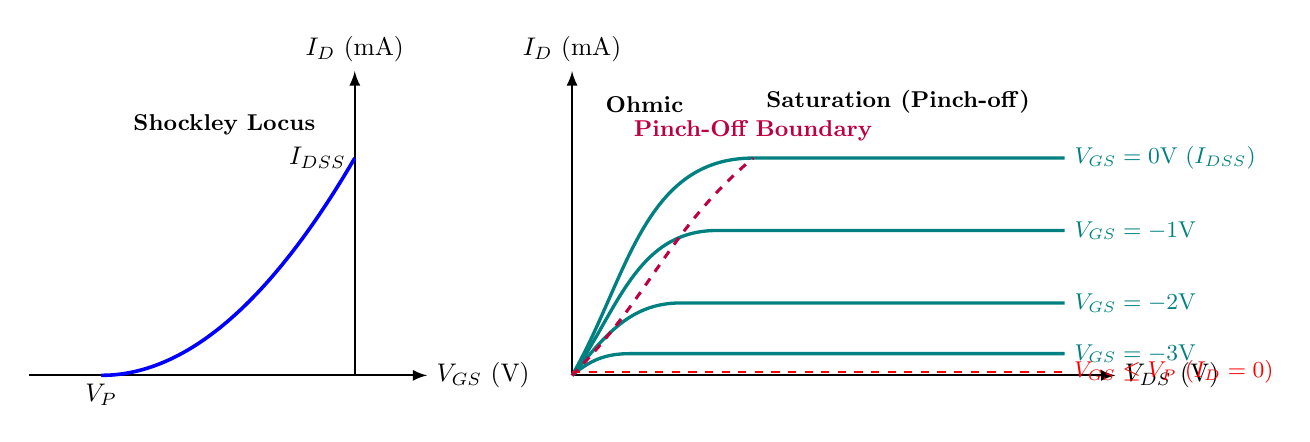
\begin{tikzpicture}[scale=0.92, transform shape]
  % Transfer Characteristics (left)
  \draw[thick, ->, >=latex] (-4.5, 0) -- (1.0, 0) node[right] {$V_{GS}\ (\text{V})$};
  \draw[thick, ->, >=latex] (0, 0) -- (0, 4.2) node[above] {$I_D\ (\text{mA})$};
  \draw[domain=-3.5:0, smooth, variable=\x, line width=1.3pt, blue] plot ({\x}, {3.0*(1 + \x/3.5)^2});
  \node[below] at (-3.5, 0) {$V_P$};
  \node[left] at (0, 3.0) {$I_{DSS}$};
  \node[above] at (-1.8, 3.2) {\small\textbf{Shockley Locus}};

  % Drain Output Characteristics (right)
  \draw[thick, ->, >=latex] (3.0, 0) -- (10.5, 0) node[right] {$V_{DS}\ (\text{V})$};
  \draw[thick, ->, >=latex] (3.0, 0) -- (3.0, 4.2) node[above] {$I_D\ (\text{mA})$};

  % Family of Curves
  \draw[line width=1.2pt, teal] (3.0, 0) to[out=60, in=180] (5.5, 3.0) -- (9.8, 3.0) node[right] {\small $V_{GS} = 0\text{V}\ (I_{DSS})$};
  \draw[line width=1.2pt, teal] (3.0, 0) to[out=55, in=180] (5.0, 2.0) -- (9.8, 2.0) node[right] {\small $V_{GS} = -1\text{V}$};
  \draw[line width=1.2pt, teal] (3.0, 0) to[out=50, in=180] (4.5, 1.0) -- (9.8, 1.0) node[right] {\small $V_{GS} = -2\text{V}$};
  \draw[line width=1.2pt, teal] (3.0, 0) to[out=40, in=180] (3.8, 0.3) -- (9.8, 0.3) node[right] {\small $V_{GS} = -3\text{V}$};
  \draw[thick, red, dashed] (3.0, 0.05) -- (9.8, 0.05) node[right] {\small $V_{GS} \le V_P\ (I_D=0)$};

  % Pinch-off locus
  \draw[dashed, purple, line width=1.1pt] (3.0, 0) to[out=45, in=-140] (5.5, 3.0) node[above=0.1cm] {\small\textbf{Pinch-Off Boundary}};
  \node[above] at (4.0, 3.5) {\small\textbf{Ohmic}};
  \node[above] at (7.5, 3.5) {\small\textbf{Saturation (Pinch-off)}};
\end{tikzpicture}
\end{schematicbox}

\paragraph{2. Conduction Equations:}
\begin{itemize}[leftmargin=1.5em]
  \item \textbf{Ohmic Region ($V_{DS} < V_{GS} - V_P$):}
  \[
  I_D = I_{DSS} \left[ 2\left(1 - \frac{V_{GS}}{V_P}\right)\frac{V_{DS}}{|V_P|} - \left(\frac{V_{DS}}{V_P}\right)^2 \right]
  \]
  \item \textbf{Saturation Region ($V_{DS} \ge V_{GS} - V_P$):}
  \[
  \mathbf{I_D = I_{DSS} \left(1 - \frac{V_{GS}}{V_P}\right)^2, \qquad g_m = \frac{2I_{DSS}}{|V_P|}\left(1 - \frac{V_{GS}}{V_P}\right)}
  \]
\end{itemize}

\begin{answerbox}
$$\mathbf{I_D = I_{DSS}\left(1 - \frac{V_{GS}}{V_P}\right)^2, \qquad V_{DS(\text{sat})} = V_{GS} - V_P}$$
\end{answerbox}

\vspace{0.6cm}

% =========================================================================
% QUESTION 4
% =========================================================================
\subsection{Question 4: N-Channel Enhancement-Type MOSFET Q-Point Calculation [7 Marks]}
\begin{questionbox}{Problem Statement (2082 Bhadra, Q4)}
Find $I_D$ and $V_{DS}$ for the circuit shown in the figure below. Given parameters are: $V_t = 1\text{ V}$ and $K = 0.48\text{ mA/V}^2$.
Circuit values: $V_{DD} = +10\text{ V}, R_1 = 11\text{ M}\Omega, R_2 = 11\text{ M}\Omega, R_D = 6\text{ k}\Omega, R_S = 6\text{ k}\Omega$.
\end{questionbox}

\begin{schematicbox}{N-Channel E-MOSFET Voltage Divider Bias Circuit}
\centering
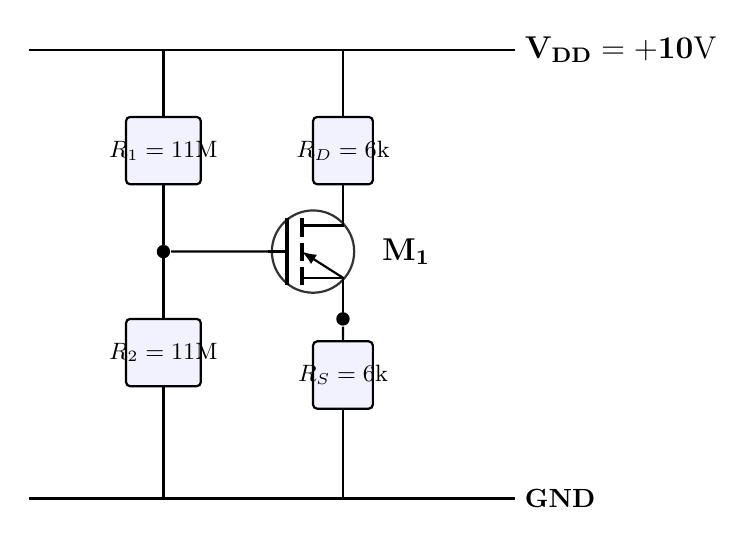
\begin{tikzpicture}[scale=0.95, transform shape]
  % Rails
  \draw[thick] (0, 5.2) -- (6.5, 5.2) node[right] {\large $\mathbf{V_{DD} = +10\text{V}}$};
  \draw[thick] (0, -0.8) -- (6.5, -0.8) node[right] {\textbf{GND}};

  % Divider R1 and R2
  \draw[thick] (1.8, 5.2) -- (1.8, 4.3);
  \draw[thick, fill=blue!5, rounded corners=1.5pt] (1.3, 3.4) rectangle (2.3, 4.3) node[midway] {\small $R_1=11\text{M}$};
  \draw[thick] (1.8, 3.4) -- (1.8, 2.5) node[circle, fill, inner sep=1.8pt] (vg) {};
  \draw[thick] (1.8, 2.5) -- (1.8, 1.6);
  \draw[thick, fill=blue!5, rounded corners=1.5pt] (1.3, 0.7) rectangle (2.3, 1.6) node[midway] {\small $R_2=11\text{M}$};
  \draw[thick] (1.8, 0.7) -- (1.8, -0.8);

  % Gate connection
  \draw[thick] (vg) -- (3.2, 2.5);

  % E-MOSFET Symbol (N-Channel)
  \draw[draw=black!80, fill=white, thick] (3.8, 2.5) circle (0.55cm);
  \draw[line width=1.4pt] (3.45, 2.05) -- (3.45, 2.95); % Gate plate
  \draw[thick] (3.2, 2.5) -- (3.45, 2.5);
  % 3 channel segments
  \draw[line width=1.6pt] (3.65, 2.7) -- (3.65, 2.95); % Drain segment
  \draw[line width=1.6pt] (3.65, 2.38) -- (3.65, 2.62); % Substrate segment
  \draw[line width=1.6pt] (3.65, 2.05) -- (3.65, 2.3); % Source segment
  % Terminals
  \draw[thick] (3.65, 2.85) -- (4.2, 2.85) -- (4.2, 3.4); % Drain
  \draw[thick] (3.65, 2.15) -- (4.2, 2.15) -- (4.2, 1.6) node[circle, fill, inner sep=1.8pt] (vs) {}; % Source
  \draw[thick, ->, >=latex] (4.2, 2.15) -- (3.65, 2.5); % Substrate arrow
  \node[right=0.2cm] at (4.4, 2.5) {\large $\mathbf{M_1}$};

  % Drain Resistor RD
  \draw[thick, fill=blue!5, rounded corners=1.5pt] (3.8, 3.4) rectangle (4.6, 4.3) node[midway] {\small $R_D=6\text{k}$};
  \draw[thick] (4.2, 4.3) -- (4.2, 5.2);

  % Source Resistor RS
  \draw[thick] (vs) -- (4.2, 1.3);
  \draw[thick, fill=blue!5, rounded corners=1.5pt] (3.8, 0.4) rectangle (4.6, 1.3) node[midway] {\small $R_S=6\text{k}$};
  \draw[thick] (4.2, 0.4) -- (4.2, -0.8);
\end{tikzpicture}
\end{schematicbox}

\paragraph{1. Gate DC Voltage ($V_G$):}
Since the insulated gate draws zero current ($I_G = 0$):
\[
V_G = V_{DD} \left(\frac{R_2}{R_1 + R_2}\right) = 10\text{ V} \times \left(\frac{11\text{ M}\Omega}{11\text{ M}\Omega + 11\text{ M}\Omega}\right) = \mathbf{5.0\text{ V}}
\]

\paragraph{2. Equation for $V_{GS}$:}
Applying KVL in the gate-source loop:
\[
V_{GS} = V_G - I_D R_S = 5.0 - 6.0 I_D \quad (\text{with } I_D \text{ in mA and } R_S = 6\text{ k}\Omega)
\]

\paragraph{3. Saturation Region Characteristic Equation:}
\[
I_D = K(V_{GS} - V_t)^2 = 0.48 \left( (5.0 - 6.0 I_D) - 1.0 \right)^2 = 0.48 (4.0 - 6.0 I_D)^2
\]
\[
I_D = 0.48 (16.0 - 48.0 I_D + 36.0 I_D^2) = 7.68 - 23.04 I_D + 17.28 I_D^2
\]
\[
\mathbf{17.28 I_D^2 - 24.04 I_D + 7.68 = 0}
\]
Solving via the quadratic formula:
\[
\Delta = (-24.04)^2 - 4(17.28)(7.68) = 577.9216 - 530.8416 = 47.0800
\]
\[
\sqrt{\Delta} = \sqrt{47.0800} = \mathbf{6.8615}
\]
\[
I_D = \frac{24.04 \pm 6.8615}{2(17.28)} = \frac{24.04 \pm 6.8615}{34.56}
\]
Two mathematical roots:
\begin{itemize}[leftmargin=1.5em]
  \item $I_{D1} = \frac{30.9015}{34.56} = 0.8941\text{ mA} \implies V_{GS1} = 5.0 - 6(0.8941) = -0.365\text{ V} < V_t = 1.0\text{ V}$ (\textbf{Invalid, below threshold}).
  \item $I_{D2} = \frac{17.1785}{34.56} = \mathbf{0.4971\text{ mA}} \implies V_{GS2} = 5.0 - 6(0.4971) = \mathbf{2.017\text{ V}} > V_t = 1.0\text{ V}$ (\textbf{Valid, transistor ON}).
\end{itemize}

\paragraph{4. Calculation of Drain-to-Source Voltage ($V_{DS}$):}
\[
V_{DS} = V_{DD} - I_D(R_D + R_S) = 10\text{ V} - 0.4971\text{ mA} \times (6\text{ k}\Omega + 6\text{ k}\Omega) = 10 - 0.4971(12.0) = \mathbf{4.035\text{ V}}
\]
\textbf{Pinch-Off (Saturation) Verification:}
\[
V_{DS} = 4.035\text{ V} \ge V_{GS} - V_t = 2.017\text{ V} - 1.0\text{ V} = 1.017\text{ V} \implies \text{Confirmed in Saturation Region!} \quad \checkmark
\]

\begin{answerbox}
$$\mathbf{I_D = 0.497\text{ mA}, \qquad V_{GS} = 2.017\text{ V}, \qquad V_{DS} = 4.035\text{ V}}$$
\end{answerbox}

\vspace{0.6cm}

% =========================================================================
% QUESTION 5
% =========================================================================
\subsection{Question 5: Barkhausen Criteria \& RC Phase Shift Oscillator [6 Marks]}
\begin{questionbox}{Problem Statement (2082 Bhadra, Q5)}
State Barkhausen criteria for sinusoidal oscillation. Explain the working principle of RC phase shift oscillator with necessary expression and circuit diagram.
\end{questionbox}

\paragraph{Part (a): Barkhausen Criteria for Sustained Sinusoidal Oscillation [2 Marks]}
For a closed-loop feedback amplifier to sustain stable sinusoidal oscillations without an external input:
\begin{enumerate}[leftmargin=1.5em]
  \item \textbf{Loop Gain Magnitude Criterion:} The magnitude of the open-loop gain must be at least unity:
  \[
  |\mathbf{A \beta}| \ge 1
  \]
  \item \textbf{Loop Phase Shift Criterion:} The total phase shift around the closed loop must be an integer multiple of $360^\circ$ ($0^\circ$):
  \[
  \angle (\mathbf{A \beta}) = 0^\circ \quad \text{or} \quad 360^\circ
  \]
\end{enumerate}

\paragraph{Part (b): Working Principle of Op-Amp RC Phase Shift Oscillator [4 Marks]}
\begin{schematicbox}{Op-Amp RC Phase Shift Oscillator Circuit}
\centering
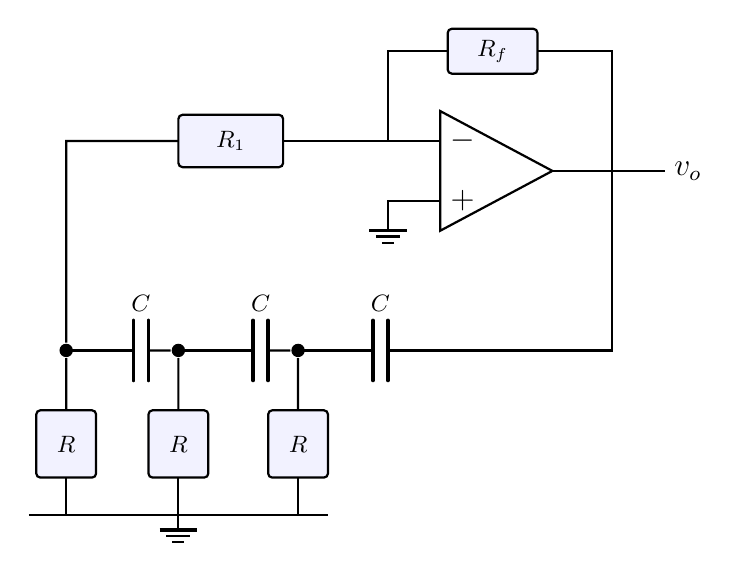
\begin{tikzpicture}[scale=0.95, transform shape]
  % Op-Amp
  \draw[thick, fill=white] (5.5, 2.0) -- (5.5, 3.6) -- (7.0, 2.8) -- cycle;
  \node at (5.8, 3.2) {\large $-$};
  \node at (5.8, 2.4) {\large $+$};
  \draw[thick] (7.0, 2.8) -- (8.5, 2.8) node[right] {\large $v_o$};

  % Non-Inverting grounded
  \draw[thick] (5.5, 2.4) -- (4.8, 2.4) -- (4.8, 2.0);
  \draw[line width=1.2pt] (4.55, 2.0) -- (5.05, 2.0);
  \draw[line width=1.0pt] (4.64, 1.92) -- (4.96, 1.92);
  \draw[line width=0.8pt] (4.72, 1.84) -- (4.88, 1.84);

  % Inverting Feedback Resistor Rf
  \draw[thick] (5.5, 3.2) -- (4.8, 3.2) -- (4.8, 4.4) -- (5.6, 4.4);
  \draw[thick, fill=blue!5, rounded corners=1.5pt] (5.6, 4.1) rectangle (6.8, 4.7) node[midway] {\small $R_f$};
  \draw[thick] (6.8, 4.4) -- (7.8, 4.4) -- (7.8, 2.8);

  % 3-Stage RC Ladder from output vo
  \draw[thick] (7.8, 2.8) -- (7.8, 0.4) -- (4.8, 0.4);

  % Stage 3 (C3, R3)
  \draw[line width=1.4pt, line cap=round] (4.8, 0.0) -- (4.8, 0.8);
  \draw[line width=1.4pt, line cap=round] (4.6, 0.0) -- (4.6, 0.8);
  \node[above] at (4.7, 0.8) {\small $C$};
  \draw[thick] (4.6, 0.4) -- (3.6, 0.4) node[circle, fill, inner sep=1.8pt] (n3) {};
  \draw[thick] (n3) -- (3.6, -0.4);
  \draw[thick, fill=blue!5, rounded corners=1.5pt] (3.2, -1.3) rectangle (4.0, -0.4) node[midway] {\small $R$};
  \draw[thick] (3.6, -1.3) -- (3.6, -1.8);

  % Stage 2 (C2, R2)
  \draw[thick] (n3) -- (3.2, 0.4);
  \draw[line width=1.4pt, line cap=round] (3.2, 0.0) -- (3.2, 0.8);
  \draw[line width=1.4pt, line cap=round] (3.0, 0.0) -- (3.0, 0.8);
  \node[above] at (3.1, 0.8) {\small $C$};
  \draw[thick] (3.0, 0.4) -- (2.0, 0.4) node[circle, fill, inner sep=1.8pt] (n2) {};
  \draw[thick] (n2) -- (2.0, -0.4);
  \draw[thick, fill=blue!5, rounded corners=1.5pt] (1.6, -1.3) rectangle (2.4, -0.4) node[midway] {\small $R$};
  \draw[thick] (2.0, -1.3) -- (2.0, -1.8);

  % Stage 1 (C1, R1)
  \draw[thick] (n2) -- (1.6, 0.4);
  \draw[line width=1.4pt, line cap=round] (1.6, 0.0) -- (1.6, 0.8);
  \draw[line width=1.4pt, line cap=round] (1.4, 0.0) -- (1.4, 0.8);
  \node[above] at (1.5, 0.8) {\small $C$};
  \draw[thick] (1.4, 0.4) -- (0.5, 0.4) node[circle, fill, inner sep=1.8pt] (n1) {};
  \draw[thick] (n1) -- (0.5, -0.4);
  \draw[thick, fill=blue!5, rounded corners=1.5pt] (0.1, -1.3) rectangle (0.9, -0.4) node[midway] {\small $R$};
  \draw[thick] (0.5, -1.3) -- (0.5, -1.8);

  % Ground bus
  \draw[thick] (0, -1.8) -- (4.0, -1.8);
  \draw[thick] (2.0, -1.8) -- (2.0, -2.0);
  \draw[line width=1.2pt] (1.75, -2.0) -- (2.25, -2.0);
  \draw[line width=1.0pt] (1.84, -2.08) -- (2.16, -2.08);
  \draw[line width=0.8pt] (1.92, -2.16) -- (2.08, -2.16);

  % Feedback to inverting input via R1
  \draw[thick] (n1) -- (0.5, 3.2) -- (2.0, 3.2);
  \draw[thick, fill=blue!5, rounded corners=1.5pt] (2.0, 2.85) rectangle (3.4, 3.55) node[midway] {\small $R_1$};
  \draw[thick] (3.4, 3.2) -- (4.8, 3.2);
\end{tikzpicture}
\end{schematicbox}

\paragraph{Mathematical Derivation of $f_0$ and Gain Requirement:}
The transfer function of the 3-stage high-pass RC ladder feedback network is:
\[
\beta(s) = \frac{v_f(s)}{v_o(s)} = \frac{s^3 R^3 C^3}{s^3 R^3 C^3 + 6s^2 R^2 C^2 + 5sRC + 1}
\]
Substituting $s = j\omega$:
\[
\beta(j\omega) = \frac{-j\omega^3 R^3 C^3}{(1 - 6\omega^2 R^2 C^2) + j(5\omega RC - \omega^3 R^3 C^3)}
\]
\begin{enumerate}[leftmargin=1.5em]
  \item \textbf{Oscillation Frequency ($f_0$):} For the feedback network to produce a $180^\circ$ phase shift, the real part in the denominator must vanish:
  \[
  1 - 6\omega_0^2 R^2 C^2 = 0 \implies \omega_0 = \frac{1}{RC\sqrt{6}} \implies \mathbf{f_0 = \frac{1}{2\pi RC\sqrt{6}}}
  \]
  \item \textbf{Feedback Attenuation at $f_0$:}
  \[
  \beta(j\omega_0) = \frac{-j(1/6\sqrt{6})}{j(5/\sqrt{6} - 1/6\sqrt{6})} = \frac{-1/6}{29/6} = -\frac{1}{29} \implies |\beta| = \frac{1}{29}
  \]
  \item \textbf{Minimum Amplifier Gain ($|A_v \beta| \ge 1$):}
  \[
  |A_v| = \frac{R_f}{R_1} \ge \frac{1}{|\beta|} = 29 \implies \mathbf{R_f \ge 29 R_1}
  \]
\end{enumerate}

\begin{answerbox}
$$\mathbf{|\mathbf{A\beta}| \ge 1, \quad \angle(\mathbf{A\beta}) = 360^\circ, \qquad f_0 = \frac{1}{2\pi RC\sqrt{6}}, \qquad |A_v| \ge 29 \implies R_f \ge 29 R_1}$$
\end{answerbox}

\vspace{0.6cm}

% =========================================================================
% QUESTION 6
% =========================================================================
\subsection{Question 6: Widlar Current Source Operation \& Advantages [5 + 2 = 7 Marks]}
\begin{questionbox}{Problem Statement (2082 Bhadra, Q6)}
With a neat circuit diagram and necessary mathematical expressions, explain the operation of Widlar current source. What is the advantage of Widlar current source over simple current source?
\end{questionbox}

\begin{schematicbox}{BJT Widlar Current Source Circuit}
\centering
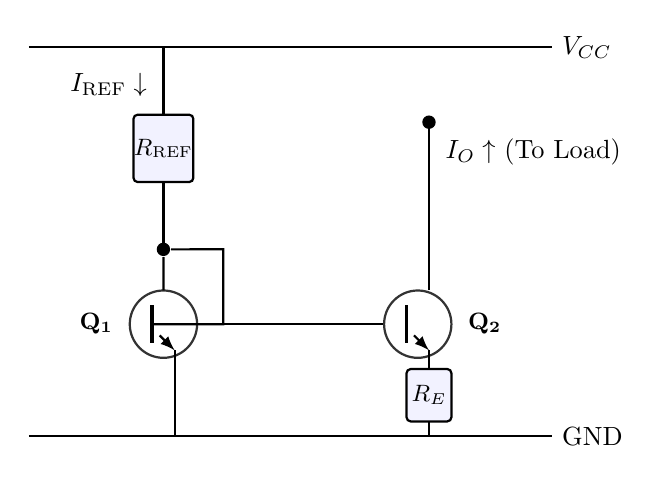
\begin{tikzpicture}[scale=0.95, transform shape]
  % Rails
  \draw[thick] (0, 5.2) -- (7.0, 5.2) node[right] {$V_{CC}$};
  \draw[thick] (0, 0) -- (7.0, 0) node[right] {GND};

  % Reference resistor R_REF
  \draw[thick] (1.8, 5.2) -- (1.8, 4.3);
  \draw[thick, fill=blue!5, rounded corners=1.5pt] (1.4, 3.4) rectangle (2.2, 4.3) node[midway] {\small $R_{\text{REF}}$};
  \draw[thick] (1.8, 3.4) -- (1.8, 2.5) node[circle, fill, inner sep=1.8pt] (n1) {};
  \node[left=0.1cm] at (1.8, 4.7) {$I_{\text{REF}} \downarrow$};

  % Transistor Q1 (Diode connected NPN)
  \draw[draw=black!80, fill=white, thick] (1.8, 1.5) circle (0.45cm);
  \draw[line width=1.4pt] (1.65, 1.25) -- (1.65, 1.75); % Base
  \draw[thick] (n1) -- (1.8, 1.95); % Collector
  \draw[thick, ->, >=latex] (1.75, 1.35) -- (1.95, 1.15); % Emitter
  \draw[thick] (1.95, 1.15) -- (1.95, 0); % To GND
  % Diode connection
  \draw[thick] (n1) -- (2.6, 2.5) -- (2.6, 1.5) -- (1.65, 1.5);
  \draw[thick] (2.6, 1.5) -- (5.05, 1.5); % Base of Q2
  \node[left=0.15cm] at (1.4, 1.5) {\small $\mathbf{Q_1}$};

  % Transistor Q2 (NPN with RE)
  \draw[draw=black!80, fill=white, thick] (5.2, 1.5) circle (0.45cm);
  \draw[line width=1.4pt] (5.05, 1.25) -- (5.05, 1.75); % Base
  \draw[thick, ->, >=latex] (5.15, 1.35) -- (5.35, 1.15); % Emitter
  \draw[thick] (5.35, 1.15) -- (5.35, 0.9);
  \draw[thick, fill=blue!5, rounded corners=1.5pt] (5.05, 0.2) rectangle (5.65, 0.9) node[midway] {\small $R_E$};
  \draw[thick] (5.35, 0.2) -- (5.35, 0);
  \draw[thick] (5.35, 1.95) -- (5.35, 4.2) node[circle, fill, inner sep=1.8pt] {};
  \node[right=0.1cm] at (5.35, 3.8) {$I_O \uparrow$ (To Load)};
  \node[right=0.15cm] at (5.6, 1.5) {\small $\mathbf{Q_2}$};
\end{tikzpicture}
\end{schematicbox}

\paragraph{Mathematical Analysis:}
\begin{enumerate}[leftmargin=1.5em]
  \item Applying KVL around the base-emitter loop of $Q_1$ and $Q_2$:
  \[
  V_{BE1} = V_{BE2} + I_{E2} R_E \approx V_{BE2} + I_O R_E \implies I_O R_E = V_{BE1} - V_{BE2}
  \]
  \item Expressing base-emitter voltages using the Ebers-Moll equation $I_C = I_S e^{V_{BE}/V_T}$:
  \[
  V_{BE1} = V_T \ln\left(\frac{I_{\text{REF}}}{I_{S1}}\right), \qquad V_{BE2} = V_T \ln\left(\frac{I_O}{I_{S2}}\right)
  \]
  Assuming matched transistors ($I_{S1} = I_{S2}$):
  \[
  \mathbf{I_O R_E = V_T \ln\left(\frac{I_{\text{REF}}}{I_O}\right) \implies R_E = \frac{V_T}{I_O} \ln\left(\frac{I_{\text{REF}}}{I_O}\right)}
  \]
\end{enumerate}

\paragraph{Part (b): Advantages over Simple Current Source [2 Marks]}
\begin{itemize}[leftmargin=1.5em]
  \item \textbf{Micro-Ampere Current Generation ($I_O \ll I_{\text{REF}}$):} Enables setting small bias currents ($\mu\text{A}$ range) using small integrated resistors ($\sim \text{k}\Omega$) rather than huge, silicon-area-prohibitive mega-ohm resistors.
  \item \textbf{Ultra-High Output Resistance:} Negative current feedback across $R_E$ increases output impedance: $R_{\text{out}} \approx r_{o2}(1 + g_{m2} R_E)$.
\end{itemize}

\begin{answerbox}
$$\mathbf{I_O R_E = V_T \ln\left(\frac{I_{\text{REF}}}{I_O}\right), \qquad R_{\text{out}} \approx r_{o2}(1 + g_{m2} R_E)}$$
\end{answerbox}

\vspace{0.6cm}

% =========================================================================
% QUESTION 7
% =========================================================================
\subsection{Question 7: Transformer-Coupled Class B Amplifier \& Minimum Efficiency [6 Marks]}
\begin{questionbox}{Problem Statement (2082 Bhadra, Q7)}
Draw the circuit diagram of transformer coupled Class B amplifier. Determine the condition for minimum efficiency of Class B amplifier.
\end{questionbox}

\begin{schematicbox}{Transformer-Coupled Class B Push-Pull Amplifier Circuit}
\centering
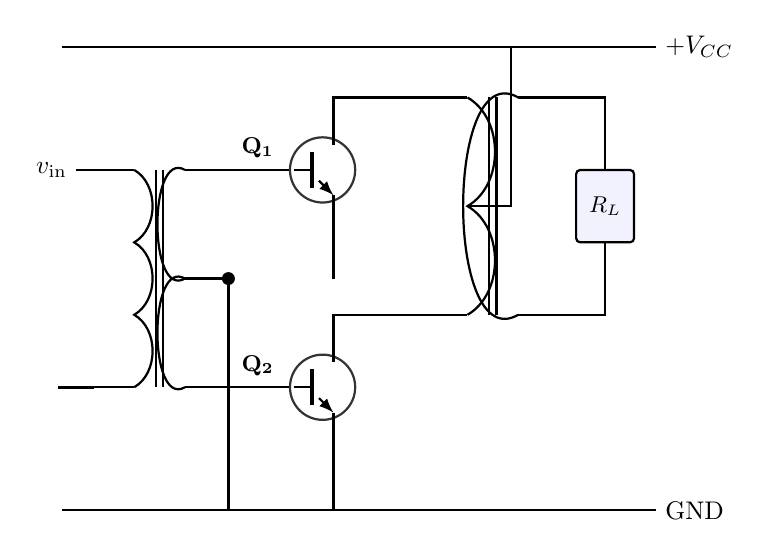
\begin{tikzpicture}[scale=0.92, transform shape]
  % Rails
  \draw[thick] (0, 5.2) -- (8.2, 5.2) node[right] {$+V_{CC}$};
  \draw[thick] (0, -1.2) -- (8.2, -1.2) node[right] {GND};

  % Input Transformer T1
  \draw[thick] (0.2, 3.5) node[left] {$v_{\text{in}}$} -- (1.0, 3.5);
  \draw[thick] (1.0, 3.5) to[out=-30, in=30] (1.0, 2.5) to[out=-30, in=30] (1.0, 1.5) to[out=-30, in=30] (1.0, 0.5);
  \draw[thick] (1.0, 0.5) -- (0.2, 0.5);
  \draw[line width=1.2pt] (-0.05, 0.5) -- (0.45, 0.5);

  % Core T1
  \draw[thick] (1.3, 3.5) -- (1.3, 0.5);
  \draw[thick] (1.4, 3.5) -- (1.4, 0.5);

  % Secondary T1 (Center Tapped)
  \draw[thick] (1.7, 3.5) to[out=150, in=-150] (1.7, 2.0) to[out=150, in=-150] (1.7, 0.5);
  \draw[thick] (1.7, 2.0) -- (2.3, 2.0) node[circle, fill, inner sep=1.8pt] {};
  \draw[thick] (2.3, 2.0) -- (2.3, -1.2); % Grounded center tap

  % Transistors Q1 and Q2 (NPN)
  \draw[thick] (1.7, 3.5) -- (3.2, 3.5);
  \draw[draw=black!80, fill=white, thick] (3.6, 3.5) circle (0.45cm);
  \draw[line width=1.4pt] (3.45, 3.25) -- (3.45, 3.75);
  \draw[thick] (3.2, 3.5) -- (3.45, 3.5);
  \draw[thick, ->, >=latex] (3.55, 3.35) -- (3.75, 3.15); % Emitter
  \draw[thick] (3.75, 3.15) -- (3.75, 2.0); % Grounded emitter
  \draw[thick] (3.75, 3.85) -- (3.75, 4.5) -- (5.6, 4.5); % Collector
  \node[left=0.15cm] at (3.2, 3.8) {\small $\mathbf{Q_1}$};

  \draw[thick] (1.7, 0.5) -- (3.2, 0.5);
  \draw[draw=black!80, fill=white, thick] (3.6, 0.5) circle (0.45cm);
  \draw[line width=1.4pt] (3.45, 0.25) -- (3.45, 0.75);
  \draw[thick] (3.2, 0.5) -- (3.45, 0.5);
  \draw[thick, ->, >=latex] (3.55, 0.35) -- (3.75, 0.15); % Emitter
  \draw[thick] (3.75, 0.15) -- (3.75, -1.2); % Grounded emitter
  \draw[thick] (3.75, 0.85) -- (3.75, 1.5) -- (5.6, 1.5); % Collector
  \node[left=0.15cm] at (3.2, 0.8) {\small $\mathbf{Q_2}$};

  % Output Transformer T2 Primary
  \draw[thick] (5.6, 4.5) to[out=-30, in=30] (5.6, 3.0) to[out=-30, in=30] (5.6, 1.5);
  \draw[thick] (5.6, 3.0) -- (6.2, 3.0) -- (6.2, 5.2); % Center tap to +VCC

  % Core T2
  \draw[thick] (5.9, 4.5) -- (5.9, 1.5);
  \draw[thick] (6.0, 4.5) -- (6.0, 1.5);

  % Secondary T2 and Load RL
  \draw[thick] (6.3, 4.5) to[out=150, in=-150] (6.3, 1.5);
  \draw[thick] (6.3, 4.5) -- (7.5, 4.5) -- (7.5, 3.5);
  \draw[thick, fill=blue!5, rounded corners=1.5pt] (7.1, 2.5) rectangle (7.9, 3.5) node[midway] {\small $R_L$};
  \draw[thick] (7.5, 2.5) -- (7.5, 1.5) -- (6.3, 1.5);
\end{tikzpicture}
\end{schematicbox}

\paragraph{Efficiency Equation and Minimum Efficiency Condition:}
\begin{enumerate}[leftmargin=1.5em]
  \item \textbf{General Efficiency Expression:}
  \[
  P_{o(\text{ac})} = \frac{V_p^2}{2 R_L'}, \qquad P_{i(\text{dc})} = \frac{2}{\pi} \frac{V_{CC} V_p}{R_L'} \implies \mathbf{\eta = \frac{\pi}{4} \left(\frac{V_p}{V_{CC}}\right) \times 100\%}
  \]
  \item \textbf{Condition for Minimum Efficiency ($\eta_{\min}$):}
  Since efficiency is directly proportional to the output voltage amplitude $V_p$:
  \[
  \text{As } V_p \to 0 \implies \mathbf{\eta_{\min} = 0\%}
  \]
  Minimum conversion efficiency ($\eta = 0\%$) occurs at **zero input signal amplitude** (quiescent no-signal condition).
  \item \textbf{Condition for Maximum Efficiency ($\eta_{\max}$):}
  Occurs when the output signal reaches maximum undistorted swing ($V_p = V_{CC}$):
  \[
  \mathbf{\eta_{\max} = \frac{\pi}{4} \times 100\% \approx 78.54\%}
  \]
\end{enumerate}

\begin{answerbox}
$$\mathbf{\eta = \frac{\pi}{4} \left(\frac{V_p}{V_{CC}}\right) \times 100\%, \qquad \eta_{\min} = 0\% \quad (\text{at } V_p = 0), \qquad \eta_{\max} = 78.54\% \quad (\text{at } V_p = V_{CC})}$$
\end{answerbox}

\vspace{0.6cm}

% =========================================================================
% QUESTION 8
% =========================================================================
\subsection{Question 8: Crossover Distortion \& Class AB Elimination [6 Marks]}
\begin{questionbox}{Problem Statement (2082 Bhadra, Q8)}
Define crossover distortion in a class B amplifier and explain how class AB operation can be used to eliminate it.
\end{questionbox}

\begin{schematicbox}{Class AB Complementary Push-Pull Amplifier with Diode Biasing}
\centering
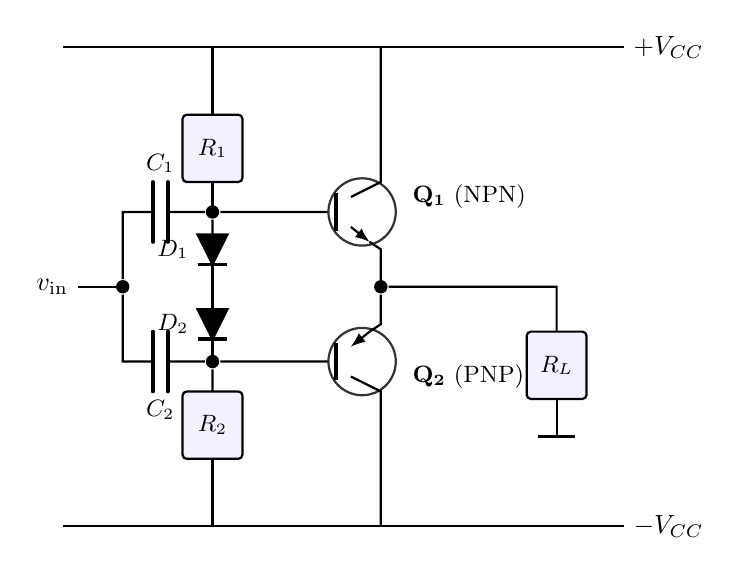
\begin{tikzpicture}[scale=0.95, transform shape]
  % Rails
  \draw[thick] (0, 5.2) -- (7.5, 5.2) node[right] {$+V_{CC}$};
  \draw[thick] (0, -1.2) -- (7.5, -1.2) node[right] {$-V_{CC}$};

  % Biasing branch
  \draw[thick] (2.0, 5.2) -- (2.0, 4.3);
  \draw[thick, fill=blue!5, rounded corners=1.5pt] (1.6, 3.4) rectangle (2.4, 4.3) node[midway] {\small $R_1$};
  \draw[thick] (2.0, 3.4) -- (2.0, 3.0) node[circle, fill, inner sep=1.8pt] (nb1) {};

  % Diodes D1 and D2
  \draw[thick] (nb1) -- (2.0, 2.7);
  \draw[thick, fill=black] (1.8, 2.7) -- (2.2, 2.7) -- (2.0, 2.3) -- cycle;
  \draw[line width=1.2pt] (1.8, 2.3) -- (2.2, 2.3);
  \node[left] at (1.8, 2.5) {\small $D_1$};
  \draw[thick] (2.0, 2.3) -- (2.0, 1.7);
  \draw[thick, fill=black] (1.8, 1.7) -- (2.2, 1.7) -- (2.0, 1.3) -- cycle;
  \draw[line width=1.2pt] (1.8, 1.3) -- (2.2, 1.3);
  \node[left] at (1.8, 1.5) {\small $D_2$};
  \draw[thick] (2.0, 1.3) -- (2.0, 1.0) node[circle, fill, inner sep=1.8pt] (nb2) {};

  \draw[thick] (nb2) -- (2.0, 0.6);
  \draw[thick, fill=blue!5, rounded corners=1.5pt] (1.6, -0.3) rectangle (2.4, 0.6) node[midway] {\small $R_2$};
  \draw[thick] (2.0, -0.3) -- (2.0, -1.2);

  % Input signal with AC coupling capacitors C1 and C2
  \draw[thick] (0.2, 2.0) node[left] {$v_{\text{in}}$} -- (0.8, 2.0) node[circle, fill, inner sep=1.8pt] (vin_node) {};
  \draw[thick] (vin_node) -- (0.8, 3.0) -- (1.2, 3.0);
  \draw[line width=1.4pt, line cap=round] (1.2, 2.6) -- (1.2, 3.4);
  \draw[line width=1.4pt, line cap=round] (1.4, 2.6) -- (1.4, 3.4);
  \node[above] at (1.3, 3.4) {\small $C_1$};
  \draw[thick] (1.4, 3.0) -- (nb1);

  \draw[thick] (vin_node) -- (0.8, 1.0) -- (1.2, 1.0);
  \draw[line width=1.4pt, line cap=round] (1.2, 0.6) -- (1.2, 1.4);
  \draw[line width=1.4pt, line cap=round] (1.4, 0.6) -- (1.4, 1.4);
  \node[below] at (1.3, 0.6) {\small $C_2$};
  \draw[thick] (1.4, 1.0) -- (nb2);

  % Transistor Q1 (NPN)
  \draw[thick] (nb1) -- (3.65, 3.0);
  \draw[draw=black!80, fill=white, thick] (4.0, 3.0) circle (0.45cm);
  \draw[line width=1.4pt] (3.65, 2.75) -- (3.65, 3.25);
  \draw[thick] (3.85, 3.2) -- (4.25, 3.4) -- (4.25, 5.2); % Collector to +VCC
  \draw[thick, ->, >=latex] (3.85, 2.8) -- (4.1, 2.6); % Emitter
  \draw[thick] (4.1, 2.6) -- (4.25, 2.5) -- (4.25, 2.0) node[circle, fill, inner sep=1.8pt] (out_node) {};
  \node[right=0.15cm] at (4.4, 3.2) {\small $\mathbf{Q_1}$ (NPN)};

  % Transistor Q2 (PNP)
  \draw[thick] (nb2) -- (3.65, 1.0);
  \draw[draw=black!80, fill=white, thick] (4.0, 1.0) circle (0.45cm);
  \draw[line width=1.4pt] (3.65, 0.75) -- (3.65, 1.25);
  \draw[thick, <-, >=latex] (3.85, 1.2) -- (4.1, 1.4); % Emitter arrow in
  \draw[thick] (4.1, 1.4) -- (4.25, 1.5) -- (out_node);
  \draw[thick] (3.85, 0.8) -- (4.25, 0.6) -- (4.25, -1.2); % Collector to -VCC
  \node[right=0.15cm] at (4.4, 0.8) {\small $\mathbf{Q_2}$ (PNP)};

  % Output to Load RL
  \draw[thick] (out_node) -- (6.6, 2.0) -- (6.6, 1.4);
  \draw[thick, fill=blue!5, rounded corners=1.5pt] (6.2, 0.5) rectangle (7.0, 1.4) node[midway] {\small $R_L$};
  \draw[thick] (6.6, 0.5) -- (6.6, 0);
  \draw[line width=1.2pt] (6.35, 0) -- (6.85, 0);
\end{tikzpicture}
\end{schematicbox}

\paragraph{1. Definition of Crossover Distortion:}
In a standard Class B push-pull stage, transistors remain unconductive whenever the input signal magnitude is below the base-emitter cut-in voltage ($|v_{\text{in}}| < 0.7\text{ V}$). This causes a flat zero-crossing interval where both transistors are completely OFF, generating severe non-linear harmonic distortion termed **crossover distortion**.

\paragraph{2. Elimination Mechanism via Class AB Biasing:}
\begin{enumerate}[leftmargin=1.5em]
  \item Diodes $D_1$ and $D_2$ establish a constant forward bias voltage $V_{BB} = V_{D1} + V_{D2} \approx 1.4\text{ V} \approx 2V_{BE}$ across the bases of $Q_1$ and $Q_2$.
  \item This trickles a small quiescent collector current ($I_{CQ} \approx 5\text{ mA} - 20\text{ mA}$) through both transistors at $v_{\text{in}} = 0\text{ V}$.
  \item Consequently, transistors transition smoothly without any zero-crossing dead-band interval, completely eliminating crossover distortion.
\end{enumerate}

\begin{answerbox}
$$\mathbf{V_{BB} = V_{D1} + V_{D2} \approx 2V_{BE} \implies \text{Completely Eliminates Zero-Crossing Dead-Band Distortion}}$$
\end{answerbox}

\vspace{0.6cm}

% =========================================================================
% QUESTION 9
% =========================================================================
\subsection{Question 9: Series Transistor Regulator with Current Limiting [5 Marks]}
\begin{questionbox}{Problem Statement (2082 Bhadra, Q9)}
Explain the working principle of a series transistor voltage regulator, accompanied by short-circuit/overload protection.
\end{questionbox}

\begin{schematicbox}{Series Transistor Voltage Regulator with Short-Circuit Current Limiting Protection}
\centering
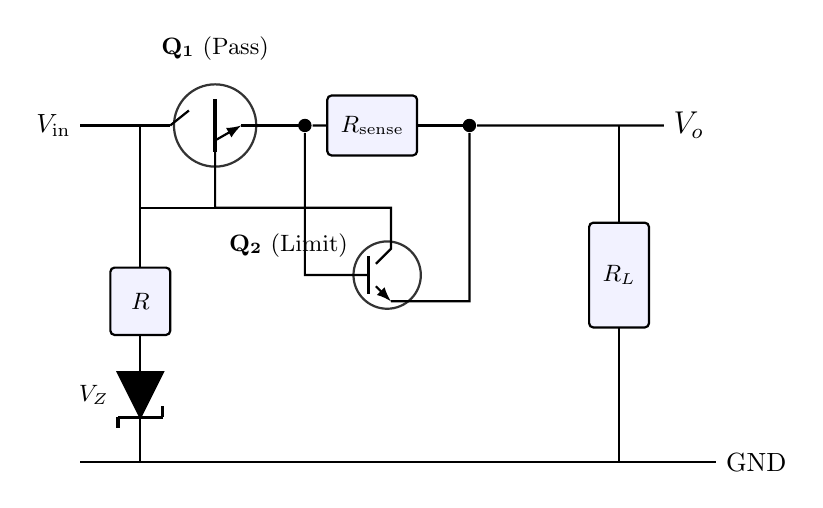
\begin{tikzpicture}[scale=0.95, transform shape]
  % Rails
  \draw[thick] (0, 4.5) node[left] {$V_{\text{in}}$} -- (1.2, 4.5);
  \draw[thick] (0, 0) -- (8.5, 0) node[right] {GND};

  % Pass Transistor Q1 (NPN)
  \draw[draw=black!80, fill=white, thick] (1.8, 4.5) circle (0.55cm);
  \draw[line width=1.6pt] (1.8, 4.15) -- (1.8, 4.85); % Base
  \draw[thick] (1.2, 4.5) -- (1.45, 4.7); % Collector
  \draw[thick, ->, >=latex] (1.8, 4.3) -- (2.15, 4.5); % Emitter
  \draw[thick] (2.15, 4.5) -- (3.0, 4.5) node[circle, fill, inner sep=1.8pt] (n_sense) {};
  \node[above=0.2cm] at (1.8, 5.05) {\small $\mathbf{Q_1}$ (Pass)};

  % Current Sensing Resistor R_sense
  \draw[thick] (n_sense) -- (3.3, 4.5);
  \draw[thick, fill=blue!5, rounded corners=1.5pt] (3.3, 4.1) rectangle (4.5, 4.9) node[midway] {\small $R_{\text{sense}}$};
  \draw[thick] (4.5, 4.5) -- (5.2, 4.5) node[circle, fill, inner sep=1.8pt] (n_out) {};
  \draw[thick] (n_out) -- (7.8, 4.5) node[right] {\large $V_o$};

  % Current Limiting Transistor Q2 (NPN)
  \draw[draw=black!80, fill=white, thick] (4.1, 2.5) circle (0.45cm);
  \draw[line width=1.4pt] (3.85, 2.25) -- (3.85, 2.75); % Base
  \draw[thick] (n_sense) -- (3.0, 2.5) -- (3.85, 2.5); % Base connected before Rsense
  \draw[thick, ->, >=latex] (3.95, 2.35) -- (4.15, 2.15); % Emitter
  \draw[thick] (4.15, 2.15) -- (5.2, 2.15) -- (n_out); % Emitter connected after Rsense
  \draw[thick] (3.95, 2.65) -- (4.15, 2.85) -- (4.15, 3.4) -- (1.8, 3.4) -- (1.8, 4.15); % Collector pulls down Q1 base
  \node[left=0.15cm] at (3.85, 2.9) {\small $\mathbf{Q_2}$ (Limit)};

  % Base bias resistor and Zener
  \draw[thick] (0.8, 4.5) -- (0.8, 3.4) -- (1.8, 3.4);
  \draw[thick] (0.8, 3.4) -- (0.8, 2.6);
  \draw[thick, fill=blue!5, rounded corners=1.5pt] (0.4, 1.7) rectangle (1.2, 2.6) node[midway] {\small $R$};
  \draw[thick] (0.8, 1.7) -- (0.8, 1.2);
  % Zener
  \draw[thick, fill=black] (0.5, 1.2) -- (1.1, 1.2) -- (0.8, 0.6) -- cycle;
  \draw[line width=1.2pt] (0.5, 0.6) -- (1.1, 0.6);
  \draw[line width=1.2pt] (0.5, 0.6) -- (0.5, 0.45);
  \draw[line width=1.2pt] (1.1, 0.6) -- (1.1, 0.75);
  \node[left] at (0.5, 0.9) {\small $V_Z$};
  \draw[thick] (0.8, 0.6) -- (0.8, 0);

  % Load Resistor
  \draw[thick] (7.2, 4.5) -- (7.2, 3.2);
  \draw[thick, fill=blue!5, rounded corners=1.5pt] (6.8, 1.8) rectangle (7.6, 3.2) node[midway] {\small $R_L$};
  \draw[thick] (7.2, 1.8) -- (7.2, 0);
\end{tikzpicture}
\end{schematicbox}

\paragraph{Working Principle and Current Limit Derivation:}
\begin{enumerate}[leftmargin=1.5em]
  \item The load current $I_L$ flows directly through $R_{\text{sense}}$, developing a voltage drop $V_{\text{sense}} = I_L R_{\text{sense}} = V_{BE2}$.
  \item \textbf{Under Normal Conditions ($I_L < I_{\text{limit}}$):}
  $V_{BE2} < 0.6\text{ V} \implies$ Protection transistor $Q_2$ remains completely OFF and does not affect the output voltage: $V_o \approx V_Z - V_{BE1}$.
  \item \textbf{Under Overload / Short-Circuit Fault ($I_L \ge I_{\text{limit}}$):}
  When $V_{\text{sense}}$ reaches the cut-in threshold ($V_{BE2} \approx 0.7\text{ V}$), transistor $Q_2$ turns ON and begins shunting excess base drive current away from pass transistor $Q_1$.
  \item Any attempt to draw more current causes $Q_2$ to conduct harder, throttling $Q_1$ and clamping the load current strictly at:
  \[
  \mathbf{I_{\text{limit}} = \frac{V_{BE2(\text{on})}}{R_{\text{sense}}} \approx \frac{0.7\text{ V}}{R_{\text{sense}}}}
  \]
\end{enumerate}

\begin{answerbox}
$$\mathbf{I_{\text{limit}} = \frac{V_{BE2}}{R_{\text{sense}}} \approx \frac{0.7\text{ V}}{R_{\text{sense}}}}$$
\end{answerbox}

\vspace{0.6cm}

% =========================================================================
% QUESTION 10
% =========================================================================
\subsection{Question 10: LM317 Adjustable Regulator Design (10V - 25V) [4 Marks]}
\begin{questionbox}{Problem Statement (2082 Bhadra, Q10)}
Design a 10-25 V variable DC voltage regulator using LM317 IC.
\end{questionbox}

\[
V_{\text{out}} = 1.25\text{ V} \left(1 + \frac{R_2}{R_1}\right)
\]
\begin{enumerate}[leftmargin=1.5em]
  \item Select standard program resistor $R_1 = \mathbf{240\ \Omega}$.
  \item For $V_{\text{out}(\min)} = 10.0\text{ V}$:
  \[
  10.0 = 1.25 \left(1 + \frac{R_{2(\min)}}{240}\right) \implies 1 + \frac{R_{2(\min)}}{240} = 8.0 \implies R_{2(\min)} = 7 \times 240 = \mathbf{1680\ \Omega} = \mathbf{1.68\text{ k}\Omega}
  \]
  \item For $V_{\text{out}(\max)} = 25.0\text{ V}$:
  \[
  25.0 = 1.25 \left(1 + \frac{R_{2(\max)}}{240}\right) \implies 1 + \frac{R_{2(\max)}}{240} = 20.0 \implies R_{2(\max)} = 19 \times 240 = \mathbf{4560\ \Omega} = \mathbf{4.56\text{ k}\Omega}
  \]
\end{enumerate}
\textbf{Practical Realization:} Use a fixed precision resistor $R_{2A} = 1.6\text{ k}\Omega$ in series with a $\mathbf{3.0\text{ k}\Omega}$ linear potentiometer ($R_2 = 1.68\text{ k}\Omega \text{ to } 4.56\text{ k}\Omega$). Input DC voltage: $V_{\text{in}} \ge 28\text{ V DC}$.

\begin{answerbox}
$$\mathbf{R_1 = 240\ \Omega, \qquad R_2 = 1.68\text{ k}\Omega \text{ to } 4.56\text{ k}\Omega \quad (\text{Fixed } 1.6\text{ k}\Omega + 3.0\text{ k}\Omega \text{ Potentiometer})}$$
\end{answerbox}

\chapter{2082 Baishakh Examination Solutions}

\section*{Examination Overview}
\begin{tabular}{@{}ll@{}}
\textbf{Level:} Bachelor in Engineering (BE) & \textbf{Full Marks:} 60 \\
\textbf{Programme:} BEI, BCT & \textbf{Pass Marks:} 24 \\
\textbf{Year / Part:} I / II & \textbf{Time:} 3 Hours \\
\textbf{Subject:} Electronic Devices \& Circuits (EX 151) & \textbf{Examination Type:} Back (New Course) \\
\end{tabular}

\vspace{0.6cm}
\hrule
\vspace{0.6cm}

% =========================================================================
% QUESTION 1
% =========================================================================
\subsection{Question 1: $\beta$-Independent Voltage Divider Bias Design [4 Marks]}
\begin{questionbox}{Problem Statement (2082 Baishakh, Q1)}
Design a $\beta$-independent voltage divider bias circuit using the appropriate guidelines for the given parameters: $V_{CC} = 12\text{V}, I_C = 1\text{mA}$, and $\beta = 100$.
\end{questionbox}

\begin{enumerate}[leftmargin=1.5em]
  \item \textbf{Emitter Voltage Allocation ($V_E$):}
  Set $V_E = 0.10 \times V_{CC} = 0.10 \times 12\text{V} = \mathbf{1.2\text{ V}}$.
  \[
  R_E = \frac{V_E}{I_E} \approx \frac{1.2\text{V}}{1.0\text{mA}} = \mathbf{1.2\text{ k}\Omega}
  \]
  \item \textbf{Collector Resistor Allocation ($R_C$):}
  Set $V_{CEQ} = \frac{V_{CC} - V_E}{2} = \frac{12 - 1.2}{2} = 5.4\text{V}$:
  \[
  R_C = \frac{V_{CC} - (V_E + V_{CEQ})}{I_C} = \frac{12 - 6.6}{1.0\text{mA}} = 5.4\text{ k}\Omega \quad (\text{Select standard } R_C = \mathbf{5.6\text{ k}\Omega})
  \]
  \item \textbf{Base Voltage Calculation ($V_B$):}
  \[
  V_B = V_E + V_{BE} = 1.2\text{V} + 0.7\text{V} = \mathbf{1.9\text{ V}}
  \]
  \item \textbf{Stiff Biasing Voltage Divider Calculation ($I_{\text{bleed}} \ge 10 I_B$):}
  \[
  I_B = \frac{1\text{mA}}{100} = 10\ \mu\text{A} \implies I_{\text{bleed}} = 100\ \mu\text{A} = 0.10\text{mA}
  \]
  \[
  R_2 = \frac{V_B}{I_{\text{bleed}}} = \frac{1.9\text{V}}{0.10\text{mA}} = \mathbf{19\text{ k}\Omega} \quad (\text{Standard } R_2 = \mathbf{18\text{ k}\Omega}\text{ or } \mathbf{20\text{ k}\Omega})
  \]
  \[
  R_1 = \frac{V_{CC} - V_B}{I_{\text{bleed}} + I_B} = \frac{12\text{V} - 1.9\text{V}}{0.11\text{mA}} = \frac{10.1\text{V}}{0.11\text{mA}} = 91.8\text{ k}\Omega \quad (\text{Standard } R_1 = \mathbf{91\text{ k}\Omega})
  \]
\end{enumerate}

\begin{schematicbox}{Designed Common Emitter Amplifier Schematic ($V_{CC} = 12\text{V}$)}
\centering
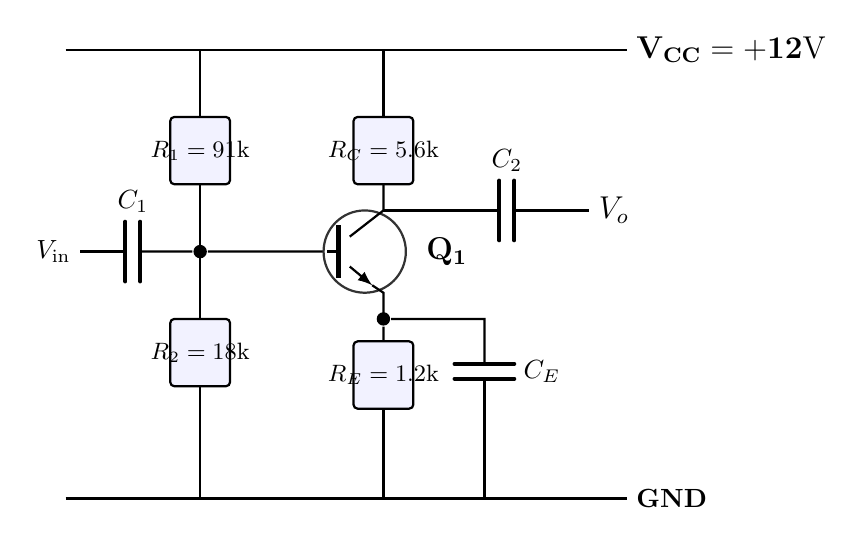
\begin{tikzpicture}[scale=0.95, transform shape]
  % Rails
  \draw[thick] (0, 5.2) -- (7.5, 5.2) node[right] {\large $\mathbf{V_{CC} = +12\text{V}}$};
  \draw[thick] (0, -0.8) -- (7.5, -0.8) node[right] {\textbf{GND}};

  % Divider R1 and R2
  \draw[thick] (1.8, 5.2) -- (1.8, 4.3);
  \draw[thick, fill=blue!5, rounded corners=1.5pt] (1.4, 3.4) rectangle (2.2, 4.3) node[midway] {\small $R_1=91\text{k}$};
  \draw[thick] (1.8, 3.4) -- (1.8, 2.5) node[circle, fill, inner sep=1.8pt] (vb) {};
  \draw[thick] (1.8, 2.5) -- (1.8, 1.6);
  \draw[thick, fill=blue!5, rounded corners=1.5pt] (1.4, 0.7) rectangle (2.2, 1.6) node[midway] {\small $R_2=18\text{k}$};
  \draw[thick] (1.8, 0.7) -- (1.8, -0.8);

  % Input coupling capacitor C1
  \draw[thick] (0.2, 2.5) node[left] {$V_{\text{in}}$} -- (0.8, 2.5);
  \draw[line width=1.4pt, line cap=round] (0.8, 2.1) -- (0.8, 2.9);
  \draw[line width=1.4pt, line cap=round] (1.0, 2.1) -- (1.0, 2.9);
  \node[above] at (0.9, 2.9) {$C_1$};
  \draw[thick] (1.0, 2.5) -- (vb);

  % Transistor Q1 (NPN)
  \draw[thick] (vb) -- (3.5, 2.5);
  \draw[draw=black!80, fill=white, thick] (4.0, 2.5) circle (0.55cm);
  \draw[line width=1.6pt] (3.65, 2.15) -- (3.65, 2.85); % Base
  \draw[thick] (3.5, 2.5) -- (3.65, 2.5);
  \draw[thick] (3.8, 2.7) -- (4.25, 3.05) -- (4.25, 3.4); % Collector
  \draw[thick, ->, >=latex] (3.8, 2.3) -- (4.1, 2.05); % Emitter
  \draw[thick] (4.1, 2.05) -- (4.25, 1.95) -- (4.25, 1.6) node[circle, fill, inner sep=1.8pt] (ve) {};
  \node[right=0.2cm] at (4.5, 2.5) {\large $\mathbf{Q_1}$};

  % Collector Resistor RC
  \draw[thick, fill=blue!5, rounded corners=1.5pt] (3.85, 3.4) rectangle (4.65, 4.3) node[midway] {\small $R_C=5.6\text{k}$};
  \draw[thick] (4.25, 4.3) -- (4.25, 5.2);

  % Emitter Resistor RE and Bypass CE
  \draw[thick] (ve) -- (4.25, 1.3);
  \draw[thick, fill=blue!5, rounded corners=1.5pt] (3.85, 0.4) rectangle (4.65, 1.3) node[midway] {\small $R_E=1.2\text{k}$};
  \draw[thick] (4.25, 0.4) -- (4.25, -0.8);

  % Bypass Capacitor CE
  \draw[thick] (ve) -- (5.6, 1.6) -- (5.6, 1.0);
  \draw[line width=1.4pt, line cap=round] (5.2, 1.0) -- (6.0, 1.0);
  \draw[line width=1.4pt, line cap=round] (5.2, 0.8) -- (6.0, 0.8);
  \node[right] at (6.0, 0.9) {$C_E$};
  \draw[thick] (5.6, 0.8) -- (5.6, -0.8);

  % Output coupling capacitor C2
  \draw[thick] (4.25, 3.05) -- (5.8, 3.05);
  \draw[line width=1.4pt, line cap=round] (5.8, 2.65) -- (5.8, 3.45);
  \draw[line width=1.4pt, line cap=round] (6.0, 2.65) -- (6.0, 3.45);
  \node[above] at (5.9, 3.45) {$C_2$};
  \draw[thick] (6.0, 3.05) -- (7.0, 3.05) node[right] {\large $V_o$};
\end{tikzpicture}
\end{schematicbox}

\begin{answerbox}
$$\mathbf{R_1 = 91\text{ k}\Omega, \quad R_2 = 18\text{ k}\Omega, \quad R_C = 5.6\text{ k}\Omega, \quad R_E = 1.2\text{ k}\Omega}$$
\end{answerbox}

\vspace{0.6cm}

% =========================================================================
% QUESTION 2
% =========================================================================
\subsection{Question 2: CE BJT Amplifier Small Signal Parameter Calculations [5 Marks]}
\begin{questionbox}{Problem Statement (2082 Baishakh, Q2)}
Determine input resistance, voltage gain and output resistance of given common emitter BJT Amplifier. $\beta = 120$ and $r_o = 40\text{ k}\Omega$.
Circuit components: $V_{CC} = 20\text{V}, R_1 = 470\text{ k}\Omega, R_2 = 56\text{ k}\Omega, R_C = 2.2\text{ k}\Omega, R_E = 0.56\text{ k}\Omega$ (with bypass capacitor $C_E$).
\end{questionbox}

\paragraph{1. DC Bias Operating Point Analysis:}
\begin{itemize}[leftmargin=1.5em]
  \item Thevenin Base Voltage:
  \[
  V_{\text{th}} = V_{CC} \left(\frac{R_2}{R_1 + R_2}\right) = 20\text{V} \times \left(\frac{56\text{k}\Omega}{470\text{k}\Omega + 56\text{k}\Omega}\right) = 20 \times \frac{56}{526} = \mathbf{2.129\text{ V}}
  \]
  \item Thevenin Resistance:
  \[
  R_{\text{th}} = R_1 \parallel R_2 = \frac{470 \times 56}{526} = \mathbf{50.038\text{ k}\Omega}
  \]
  \item Quiescent Base and Emitter Currents:
  \[
  I_B = \frac{V_{\text{th}} - V_{BE}}{R_{\text{th}} + (1+\beta)R_E} = \frac{2.129\text{V} - 0.7\text{V}}{50.038\text{k}\Omega + (121)(0.56\text{k}\Omega)} = \frac{1.429\text{V}}{50.038\text{k}\Omega + 67.76\text{k}\Omega} = \frac{1.429\text{V}}{117.8\text{k}\Omega} = \mathbf{12.13\ \mu\text{A}}
  \]
  \[
  I_E = (1+\beta)I_B = 121 \times 12.13\ \mu\text{A} = \mathbf{1.468\text{ mA}}
  \]
  \item Dynamic Emitter Resistance:
  \[
  r_e = \frac{V_T}{I_E} = \frac{26\text{ mV}}{1.468\text{ mA}} = \mathbf{17.71\ \Omega}
  \]
\end{itemize}

\paragraph{2. Small-Signal AC Parameters:}
\begin{enumerate}[leftmargin=1.5em]
  \item \textbf{Input Resistance ($R_{\text{in}}$):}
  \[
  Z_b = \beta r_e = 120 \times 17.71\ \Omega = \mathbf{2.125\text{ k}\Omega}
  \]
  \[
  R_{\text{in}} = R_1 \parallel R_2 \parallel Z_b = 50.038\text{k}\Omega \parallel 2.125\text{k}\Omega = \frac{50.038 \times 2.125}{52.163} = \mathbf{2.038\text{ k}\Omega}
  \]
  \item \textbf{Output Resistance ($R_{\text{out}}$):}
  \[
  R_{\text{out}} = R_C \parallel r_o = 2.2\text{k}\Omega \parallel 40\text{k}\Omega = \frac{2.2 \times 40}{42.2} = \mathbf{2.085\text{ k}\Omega}
  \]
  \item \textbf{Voltage Gain ($A_v$):}
  \[
  A_v = -\frac{R_C \parallel r_o}{r_e} = -\frac{2085.3\ \Omega}{17.71\ \Omega} = \mathbf{-117.75} \quad (180^\circ \text{ phase inversion})
  \]
\end{enumerate}

\begin{answerbox}
$$\mathbf{R_{\text{in}} = 2.038\text{ k}\Omega, \qquad R_{\text{out}} = 2.085\text{ k}\Omega, \qquad A_v = -117.75}$$
\end{answerbox}

\vspace{0.6cm}

% =========================================================================
% QUESTION 3
% =========================================================================
\subsection{Question 3: BJT Operation as a Switch \& Dynamic Switching Times [4 Marks]}
\begin{questionbox}{Problem Statement (2082 Baishakh, Q3)}
Explain the operation principle of a BJT as a switch with the necessary diagrams.
\end{questionbox}

\paragraph{1. Operating States of BJT as a Switch:}
\begin{itemize}[leftmargin=1.5em]
  \item \textbf{OFF State (Cutoff Region):} $V_{\text{in}} \le 0\text{V} \implies I_B = 0 \implies I_C \approx 0$. Transistor behaves as an open contact; $V_{CE} = V_{CC}$.
  \item \textbf{ON State (Saturation Region):} $V_{\text{in}} \gg V_{BE} \implies I_B \ge I_{B(\text{sat})} = \frac{I_{C(\text{sat})}}{\beta_{\min}}$. Transistor behaves as a closed contact; $V_{CE} = V_{CE(\text{sat})} \approx 0.1\text{V} - 0.2\text{V}$.
\end{itemize}

\paragraph{2. Transient Switching Times:}
\begin{schematicbox}{BJT Dynamic Switching Waveforms and Interval Definitions}
\centering
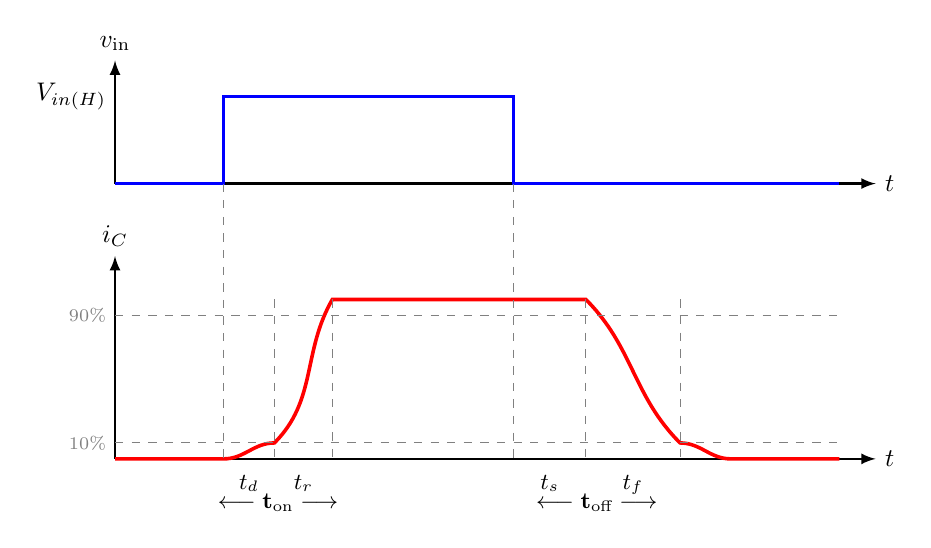
\begin{tikzpicture}[scale=0.92, transform shape]
  % Input pulse
  \draw[thick, ->, >=latex] (0, 3.8) -- (10.5, 3.8) node[right] {$t$};
  \draw[thick, ->, >=latex] (0, 3.8) -- (0, 5.5) node[above] {$v_{\text{in}}$};
  \draw[line width=1.2pt, blue] (0, 3.8) -- (1.5, 3.8) -- (1.5, 5.0) -- (5.5, 5.0) -- (5.5, 3.8) -- (10.0, 3.8);
  \node[left] at (0, 5.0) {$V_{in(H)}$};

  % Output Collector Current waveform
  \draw[thick, ->, >=latex] (0, 0) -- (10.5, 0) node[right] {$t$};
  \draw[thick, ->, >=latex] (0, 0) -- (0, 2.8) node[above] {$i_C$};
  \draw[line width=1.3pt, red] (0, 0) -- (1.5, 0) to[out=0, in=180] (2.2, 0.22) to[out=45, in=-120] (3.0, 2.2) -- (5.5, 2.2) to[out=0, in=180] (6.5, 2.2) to[out=-45, in=135] (7.8, 0.22) to[out=0, in=180] (8.5, 0) -- (10.0, 0);

  % 10% and 90% lines
  \draw[dashed, gray] (0, 0.22) node[left] {\scriptsize $10\%$} -- (10.0, 0.22);
  \draw[dashed, gray] (0, 1.98) node[left] {\scriptsize $90\%$} -- (10.0, 1.98);

  % Annotations
  \draw[dashed, gray] (1.5, 3.8) -- (1.5, 0);
  \draw[dashed, gray] (2.2, 2.2) -- (2.2, 0);
  \draw[dashed, gray] (3.0, 2.2) -- (3.0, 0);
  \node[below=0.1cm] at (1.85, 0) {\small $t_d$};
  \node[below=0.1cm] at (2.6, 0) {\small $t_r$};
  \node[above] at (2.25, -0.85) {\small $\mathbf{\longleftarrow t_{\text{on}} \longrightarrow}$};

  \draw[dashed, gray] (5.5, 3.8) -- (5.5, 0);
  \draw[dashed, gray] (6.5, 2.2) -- (6.5, 0);
  \draw[dashed, gray] (7.8, 2.2) -- (7.8, 0);
  \node[below=0.1cm] at (6.0, 0) {\small $t_s$};
  \node[below=0.1cm] at (7.15, 0) {\small $t_f$};
  \node[above] at (6.65, -0.85) {\small $\mathbf{\longleftarrow t_{\text{off}} \longrightarrow}$};
\end{tikzpicture}
\end{schematicbox}

\begin{itemize}[leftmargin=1.5em]
  \item \textbf{Turn-On Time ($t_{\text{on}} = t_d + t_r$):} Delay time $t_d$ (junction capacitance charging) + Rise time $t_r$ ($10\%$ to $90\%$ of $I_C$).
  \item \textbf{Turn-Off Time ($t_{\text{off}} = t_s + t_f$):} Storage time $t_s$ (removal of excess stored base charge) + Fall time $t_f$ ($90\%$ down to $10\%$).
\end{itemize}

\begin{answerbox}
BJT acts as an inverter switch between Cutoff ($V_{CE}=V_{CC}$) and Saturation ($V_{CE}\approx 0.2\text{V}$), with total switching speed governed by $t_{\text{on}} = t_d + t_r$ and $t_{\text{off}} = t_s + t_f$.
\end{answerbox}

\vspace{0.6cm}

% =========================================================================
% QUESTION 4
% =========================================================================
\subsection{Question 4: N-Channel Depletion-Type MOSFET [7 Marks]}
\begin{questionbox}{Problem Statement (2082 Baishakh, Q4)}
Describe the construction and working principle of n-channel depletion type MOSFET with the help of characteristics curve and mathematical expressions.
\end{questionbox}

\paragraph{1. Physical Construction:}
An N-Channel Depletion-Type MOSFET (D-MOSFET) is built on a p-type silicon substrate:
\begin{itemize}[leftmargin=1.5em]
  \item Two heavily doped $n^+$ regions form the \textbf{Source} and \textbf{Drain}.
  \item A physical, chemically doped \textbf{n-type channel} is pre-diffused between source and drain during fabrication.
  \item The \textbf{Gate} terminal is completely insulated from the channel by a dielectric layer of Silicon Dioxide ($\text{SiO}_2$).
\end{itemize}

\paragraph{2. Working Principle:}
\begin{enumerate}[leftmargin=1.5em]
  \item \textbf{Depletion Mode ($V_{GS} < 0$):} Applying a negative gate voltage repels conduction electrons from the n-channel into the p-substrate, creating a depletion region and reducing drain current $I_D$. At $V_{GS} = V_P$ (Pinch-off voltage), the channel is fully depleted and $I_D = 0$.
  \item \textbf{Enhancement Mode ($V_{GS} > 0$):} Applying a positive gate voltage attracts additional free electrons from the substrate into the channel, enhancing channel conductivity and increasing $I_D$ above $I_{DSS}$.
\end{enumerate}

\begin{schematicbox}{Transfer and Drain Characteristic Curves of N-Channel D-MOSFET}
\centering
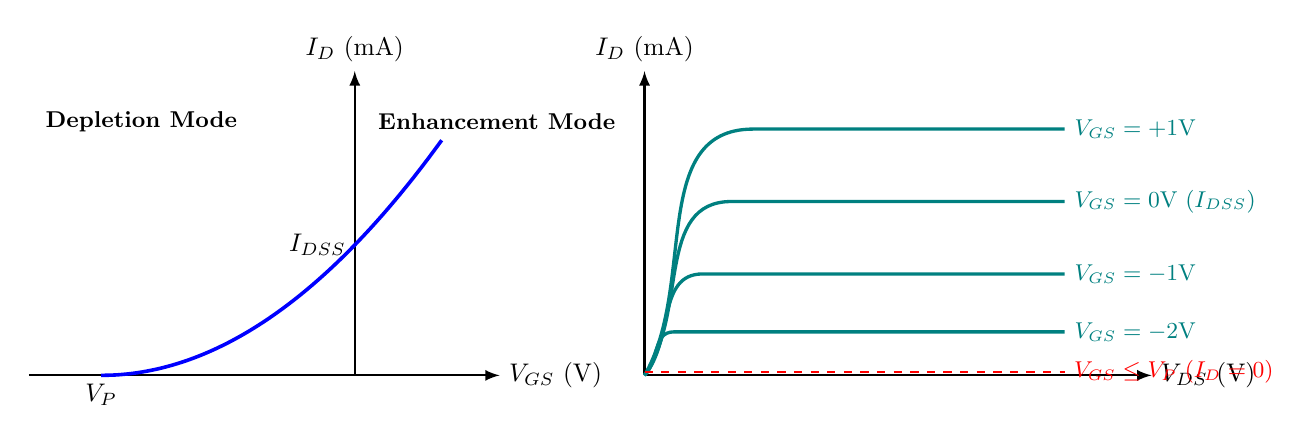
\begin{tikzpicture}[scale=0.92, transform shape]
  % Transfer Characteristics (left)
  \draw[thick, ->, >=latex] (-4.5, 0) -- (2.0, 0) node[right] {$V_{GS}\ (\text{V})$};
  \draw[thick, ->, >=latex] (0, 0) -- (0, 4.2) node[above] {$I_D\ (\text{mA})$};
  \draw[domain=-3.5:1.2, smooth, variable=\x, line width=1.3pt, blue] plot ({\x}, {1.8*(1 + \x/3.5)^2});
  \node[below] at (-3.5, 0) {$V_P$};
  \node[left] at (0, 1.8) {$I_{DSS}$};
  \node[left] at (-1.5, 3.5) {\small\textbf{Depletion Mode}};
  \node[right] at (0.2, 3.5) {\small\textbf{Enhancement Mode}};

  % Drain Characteristics (right)
  \draw[thick, ->, >=latex] (4.0, 0) -- (11.0, 0) node[right] {$V_{DS}\ (\text{V})$};
  \draw[thick, ->, >=latex] (4.0, 0) -- (4.0, 4.2) node[above] {$I_D\ (\text{mA})$};
  \draw[line width=1.2pt, teal] (4.0, 0) to[out=60, in=180] (5.5, 3.4) -- (9.8, 3.4) node[right] {\small $V_{GS} = +1\text{V}$};
  \draw[line width=1.2pt, teal] (4.0, 0) to[out=55, in=180] (5.2, 2.4) -- (9.8, 2.4) node[right] {\small $V_{GS} = 0\text{V}\ (I_{DSS})$};
  \draw[line width=1.2pt, teal] (4.0, 0) to[out=50, in=180] (4.8, 1.4) -- (9.8, 1.4) node[right] {\small $V_{GS} = -1\text{V}$};
  \draw[line width=1.2pt, teal] (4.0, 0) to[out=45, in=180] (4.4, 0.6) -- (9.8, 0.6) node[right] {\small $V_{GS} = -2\text{V}$};
  \draw[thick, red, dashed] (4.0, 0.05) -- (9.8, 0.05) node[right] {\small $V_{GS} \le V_P\ (I_D=0)$};
\end{tikzpicture}
\end{schematicbox}

\paragraph{3. Mathematical Model (Shockley's Equation):}
In the saturation (active) region ($V_{DS} \ge V_{GS} - V_P$):
\[
\mathbf{I_D = I_{DSS} \left(1 - \frac{V_{GS}}{V_P}\right)^2} \quad \text{valid for both } V_{GS} \le 0 \text{ and } V_{GS} > 0
\]

\begin{answerbox}
$$\mathbf{I_D = I_{DSS}\left(1 - \frac{V_{GS}}{V_P}\right)^2, \qquad g_m = \frac{2I_{DSS}}{|V_P|}\left(1 - \frac{V_{GS}}{V_P}\right)}$$
\end{answerbox}

\vspace{0.6cm}

% =========================================================================
% QUESTION 5
% =========================================================================
\subsection{Question 5: JFET Voltage Divider Bias Q-Point \& Transconductance [6 Marks]}
\begin{questionbox}{Problem Statement (2082 Baishakh, Q5)}
For the given JFET voltage divider configuration, determine $I_{DQ}, V_{GSQ}, V_{DS}$ and transconductance $g_m$.
Given parameters: $V_{DD} = 20\text{V}, R_1 = 910\text{ k}\Omega, R_2 = 110\text{ k}\Omega, R_D = 2.2\text{ k}\Omega, R_S = 1.1\text{ k}\Omega, I_{DSS} = 10\text{mA}, V_P = -3.5\text{V}$.
\end{questionbox}

\paragraph{1. Gate Voltage Calculation ($V_G$):}
\[
V_G = V_{DD} \left(\frac{R_2}{R_1 + R_2}\right) = 20\text{V} \times \left(\frac{110\text{k}\Omega}{910\text{k}\Omega + 110\text{k}\Omega}\right) = 20 \times \frac{110}{1020} = \mathbf{2.1569\text{ V}}
\]

\paragraph{2. Equation for $V_{GS}$:}
\[
V_{GS} = V_G - I_D R_S = 2.1569 - 1.1 I_D \quad (\text{with } I_D \text{ in mA})
\]

\paragraph{3. Substitution into Shockley's Law:}
\[
I_D = 10 \left(1 - \frac{2.1569 - 1.1 I_D}{-3.5}\right)^2 = 10 \left(\frac{3.5 + 2.1569 - 1.1 I_D}{3.5}\right)^2 = \frac{10}{12.25} (5.6569 - 1.1 I_D)^2
\]
\[
1.225 I_D = 32.0 - 12.445 I_D + 1.21 I_D^2 \implies 1.21 I_D^2 - 13.67 I_D + 32.0 = 0
\]
Solving via quadratic formula:
\[
I_D = \frac{13.67 \pm \sqrt{(13.67)^2 - 4(1.21)(32.0)}}{2(1.21)} = \frac{13.67 \pm \sqrt{186.87 - 154.88}}{2.42} = \frac{13.67 \pm 5.656}{2.42}
\]
Two roots:
\begin{itemize}[leftmargin=1.5em]
  \item $I_{D1} = 7.986\text{ mA} \implies V_{GS1} = 2.1569 - 1.1(7.986) = -6.628\text{V} < V_P$ (\textbf{Invalid}).
  \item $I_{D2} = \mathbf{3.312\text{ mA}} \implies V_{GS2} = 2.1569 - 1.1(3.312) = \mathbf{-1.486\text{ V}}$ (\textbf{Valid}, since $-3.5\text{V} \le V_{GS} \le 0$).
\end{itemize}

\paragraph{4. Calculation of $V_{DS}$ and Transconductance $g_m$:}
\[
V_{DS} = V_{DD} - I_D(R_D + R_S) = 20\text{V} - 3.312\text{mA} \times (2.2\text{k}\Omega + 1.1\text{k}\Omega) = 20 - 3.312(3.3) = \mathbf{9.07\text{ V}}
\]
\[
g_m = \frac{2 I_{DSS}}{|V_P|} \left(1 - \frac{V_{GSQ}}{V_P}\right) = \frac{2 \times 10\text{mA}}{3.5\text{V}} \left(1 - \frac{-1.486\text{V}}{-3.5\text{V}}\right) = 5.714 \times (1 - 0.4246) = \mathbf{3.288\text{ mS}}
\]

\begin{answerbox}
$$\mathbf{I_{DQ} = 3.312\text{ mA}, \qquad V_{GSQ} = -1.486\text{ V}, \qquad V_{DS} = 9.07\text{ V}, \qquad g_m = 3.288\text{ mS}}$$
\end{answerbox}

\vspace{0.6cm}

% =========================================================================
% QUESTION 6
% =========================================================================
\subsection{Question 6: LC Hartley Oscillator Frequency Derivation [4 Marks]}
\begin{questionbox}{Problem Statement (2082 Baishakh, Q6)}
Draw circuit diagram of LC Hartley oscillator. Derive its frequency of oscillation.
\end{questionbox}

A Hartley oscillator employs an inductive voltage divider with two tapped inductors ($L_1, L_2$) having mutual inductance $M$, tuned by capacitor $C$.

\begin{schematicbox}{BJT LC Hartley Oscillator Circuit}
\centering
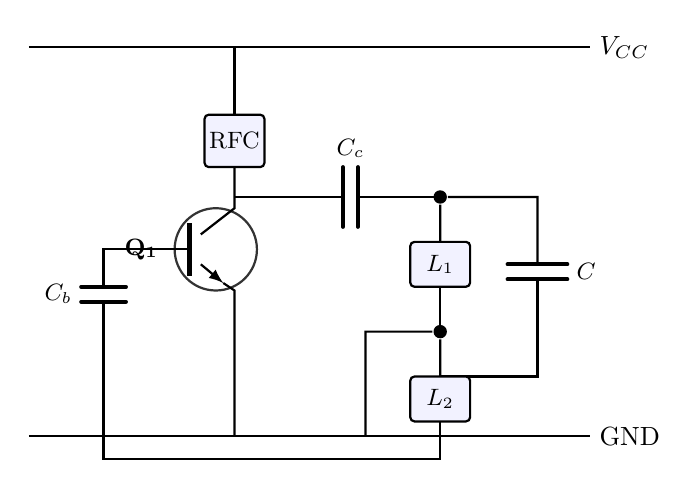
\begin{tikzpicture}[scale=0.95, transform shape]
  % Rails
  \draw[thick] (0, 5.2) -- (7.5, 5.2) node[right] {$V_{CC}$};
  \draw[thick] (0, 0) -- (7.5, 0) node[right] {GND};

  % BJT Transistor Q1 (NPN)
  \draw[draw=black!80, fill=white, thick] (2.5, 2.5) circle (0.55cm);
  \draw[line width=1.6pt] (2.15, 2.15) -- (2.15, 2.85); % Base
  \draw[thick] (2.15, 2.5) -- (1.5, 2.5); % Base lead
  \draw[thick] (2.3, 2.7) -- (2.75, 3.05) -- (2.75, 3.6); % Collector
  \draw[thick, ->, >=latex] (2.3, 2.3) -- (2.6, 2.05); % Emitter
  \draw[thick] (2.6, 2.05) -- (2.75, 1.95) -- (2.75, 0); % Emitter to GND
  \node[left=0.15cm] at (2.0, 2.5) {\small $\mathbf{Q_1}$};

  % Radio Frequency Choke (RFC)
  \draw[thick] (2.75, 3.6) -- (2.75, 4.3);
  \draw[thick, fill=blue!5, rounded corners=1.5pt] (2.35, 3.6) rectangle (3.15, 4.3) node[midway] {\small RFC};
  \draw[thick] (2.75, 4.3) -- (2.75, 5.2);

  % Output to Tank coupling capacitor
  \draw[thick] (2.75, 3.2) -- (4.2, 3.2);
  \draw[line width=1.4pt, line cap=round] (4.2, 2.8) -- (4.2, 3.6);
  \draw[line width=1.4pt, line cap=round] (4.4, 2.8) -- (4.4, 3.6);
  \node[above] at (4.3, 3.6) {\small $C_c$};
  \draw[thick] (4.4, 3.2) -- (5.5, 3.2) node[circle, fill, inner sep=1.8pt] (tank_top) {};

  % Tank tuning capacitor C
  \draw[thick] (tank_top) -- (6.8, 3.2) -- (6.8, 2.3);
  \draw[line width=1.4pt, line cap=round] (6.4, 2.3) -- (7.2, 2.3);
  \draw[line width=1.4pt, line cap=round] (6.4, 2.1) -- (7.2, 2.1);
  \node[right] at (7.2, 2.2) {\small $C$};
  \draw[thick] (6.8, 2.1) -- (6.8, 0.8) -- (5.5, 0.8);

  % Tapped Inductors L1 and L2
  \draw[thick] (tank_top) -- (5.5, 2.6);
  \draw[thick, fill=blue!5, rounded corners=1.5pt] (5.1, 2.0) rectangle (5.9, 2.6) node[midway] {\small $L_1$};
  \draw[thick] (5.5, 2.0) -- (5.5, 1.4) node[circle, fill, inner sep=1.8pt] (tap) {};
  \draw[thick] (tap) -- (4.5, 1.4) -- (4.5, 0); % Grounded center tap
  \draw[thick] (tap) -- (5.5, 0.8);
  \draw[thick, fill=blue!5, rounded corners=1.5pt] (5.1, 0.2) rectangle (5.9, 0.8) node[midway] {\small $L_2$};
  \draw[thick] (5.5, 0.2) -- (5.5, -0.3) -- (1.0, -0.3) -- (1.0, 1.8);
  \draw[line width=1.4pt, line cap=round] (0.7, 1.8) -- (1.3, 1.8);
  \draw[line width=1.4pt, line cap=round] (0.7, 2.0) -- (1.3, 2.0);
  \node[left] at (0.7, 1.9) {\small $C_b$};
  \draw[thick] (1.0, 2.0) -- (1.0, 2.5) -- (1.5, 2.5); % Feedback to base
\end{tikzpicture}
\end{schematicbox}

\paragraph{Derivation of Oscillation Frequency:}
The feedback factor is given by $\beta = \frac{X_{L2}}{X_{L1}} = \frac{L_2 + M}{L_1 + M}$.\\
The equivalent tank inductance of the series tapped inductor is:
\[
L_{\text{eq}} = L_1 + L_2 + 2M
\]
The resonant frequency where inductive and capacitive reactances cancel ($X_{L_{\text{eq}}} = X_C$) is:
\[
\omega_0 L_{\text{eq}} = \frac{1}{\omega_0 C} \implies \omega_0^2 = \frac{1}{L_{\text{eq}} C} \implies \mathbf{f_0 = \frac{1}{2\pi \sqrt{(L_1 + L_2 + 2M)C}}}
\]

\begin{answerbox}
$$\mathbf{f_0 = \frac{1}{2\pi \sqrt{(L_1 + L_2 + 2M)C}}}$$
\end{answerbox}

\vspace{0.6cm}

% =========================================================================
% QUESTION 7
% =========================================================================
\subsection{Question 7: Bandwidth of Class A Tuned Amplifier [4 Marks]}
\begin{questionbox}{Problem Statement (2082 Baishakh, Q7)}
Derive the expression of bandwidth of class A tuned amplifier.
\end{questionbox}

A tuned amplifier uses a parallel LC tank circuit as its collector load. At the resonant frequency $f_0 = \frac{1}{2\pi\sqrt{LC}}$, the impedance is purely resistive: $R_p = Q^2 R_s = \frac{L}{C R_s}$.

\begin{schematicbox}{Frequency Response Curve of Tuned Amplifier}
\centering
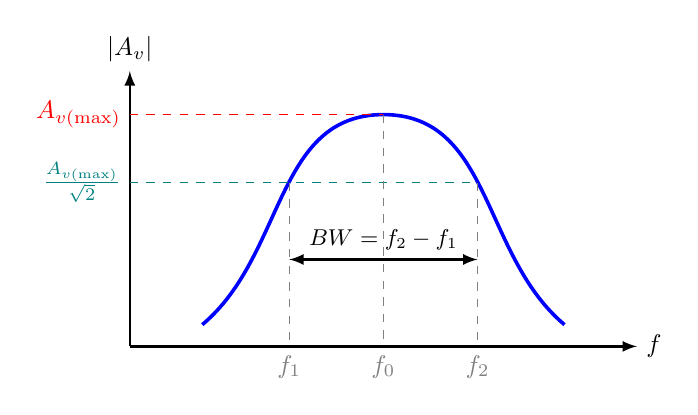
\begin{tikzpicture}[scale=0.92, transform shape]
  \draw[thick, ->, >=latex] (0, 0) -- (7.0, 0) node[right] {$f$};
  \draw[thick, ->, >=latex] (0, 0) -- (0, 3.8) node[above] {$|A_v|$};
  \draw[line width=1.3pt, blue] (1.0, 0.3) to[out=40, in=180] (3.5, 3.2) to[out=0, in=140] (6.0, 0.3);

  \draw[dashed, red] (0, 3.2) node[left] {$A_{v(\max)}$} -- (3.5, 3.2);
  \draw[dashed, teal] (0, 2.26) node[left] {$\frac{A_{v(\max)}}{\sqrt{2}}$} -- (4.8, 2.26);
  \draw[dashed, gray] (2.2, 2.26) -- (2.2, 0) node[below] {$f_1$};
  \draw[dashed, gray] (3.5, 3.2) -- (3.5, 0) node[below] {$f_0$};
  \draw[dashed, gray] (4.8, 2.26) -- (4.8, 0) node[below] {$f_2$};

  \draw[thick, <->, >=latex] (2.2, 1.2) -- (4.8, 1.2) node[midway, above] {\small $BW = f_2 - f_1$};
\end{tikzpicture}
\end{schematicbox}

\begin{itemize}[leftmargin=1.5em]
  \item The $3\text{dB}$ half-power frequencies ($f_1$ and $f_2$) occur where the tank impedance falls to $\frac{R_p}{\sqrt{2}}$.
  \item The Quality Factor ($Q$) of the resonant circuit is defined as:
  \[
  Q = \frac{\omega_0 L}{R} = \frac{f_0}{BW} \implies \mathbf{BW = f_2 - f_1 = \frac{f_0}{Q} = \frac{1}{2\pi R_p C}}
  \]
\end{itemize}

\begin{answerbox}
$$\mathbf{BW = \frac{f_0}{Q}}$$
\end{answerbox}

\vspace{0.6cm}

% =========================================================================
% QUESTION 8
% =========================================================================
\subsection{Question 8: Differential Amplifier with Active vs. Passive Load [5 Marks]}
\begin{questionbox}{Problem Statement (2082 Baishakh, Q8)}
Show that the voltage gain of the differential amplifier with active load is twice that with passive load.
\end{questionbox}

\begin{schematicbox}{Differential Amplifier with Active Current Mirror Load}
\centering
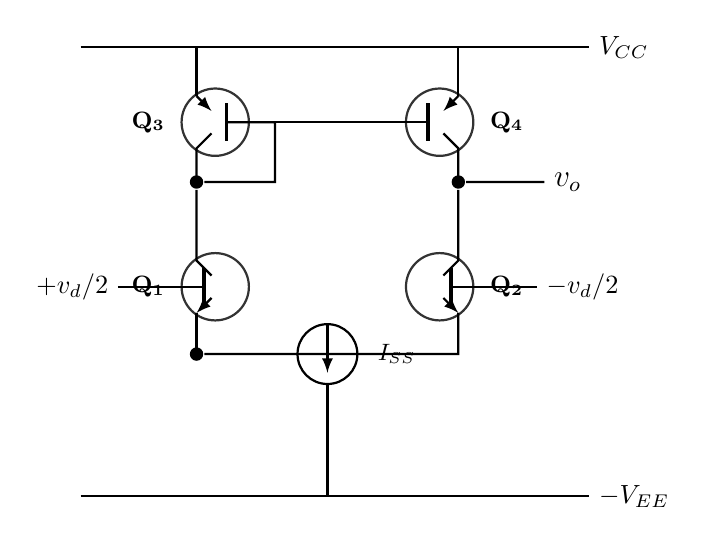
\begin{tikzpicture}[scale=0.95, transform shape]
  % Rails
  \draw[thick] (0, 5.2) -- (6.8, 5.2) node[right] {$V_{CC}$};
  \draw[thick] (0, -0.8) -- (6.8, -0.8) node[right] {$-V_{EE}$};

  % Active PMOS/PNP Current Mirror Load (Q3, Q4)
  \draw[draw=black!80, fill=white, thick] (1.8, 4.2) circle (0.45cm);
  \draw[line width=1.4pt] (1.95, 3.95) -- (1.95, 4.45); % Base
  \draw[thick, <-, >=latex] (1.75, 4.35) -- (1.55, 4.55); % Emitter in
  \draw[thick] (1.55, 4.55) -- (1.55, 5.2);
  \draw[thick] (1.75, 4.05) -- (1.55, 3.85) -- (1.55, 3.4) node[circle, fill, inner sep=1.8pt] (n_c3) {};
  \node[left=0.15cm] at (1.4, 4.2) {\small $\mathbf{Q_3}$};

  \draw[draw=black!80, fill=white, thick] (4.8, 4.2) circle (0.45cm);
  \draw[line width=1.4pt] (4.65, 3.95) -- (4.65, 4.45); % Base
  \draw[thick, <-, >=latex] (4.85, 4.35) -- (5.05, 4.55); % Emitter in
  \draw[thick] (5.05, 4.55) -- (5.05, 5.2);
  \draw[thick] (4.85, 4.05) -- (5.05, 3.85) -- (5.05, 3.4) node[circle, fill, inner sep=1.8pt] (n_out) {};
  \node[right=0.15cm] at (5.2, 4.2) {\small $\mathbf{Q_4}$};

  % Diode connection for Q3 and mirror bus
  \draw[thick] (1.95, 4.2) -- (2.6, 4.2) -- (2.6, 3.4) -- (n_c3);
  \draw[thick] (2.6, 4.2) -- (4.65, 4.2);

  % Differential Input Pair (Q1, Q2)
  \draw[draw=black!80, fill=white, thick] (1.8, 2.0) circle (0.45cm);
  \draw[line width=1.4pt] (1.65, 1.75) -- (1.65, 2.25); % Base
  \draw[thick] (0.5, 2.0) node[left] {$+v_d/2$} -- (1.65, 2.0);
  \draw[thick] (1.75, 2.15) -- (1.55, 2.35) -- (n_c3);
  \draw[thick, ->, >=latex] (1.75, 1.85) -- (1.55, 1.65); % Emitter
  \draw[thick] (1.55, 1.65) -- (1.55, 1.1) node[circle, fill, inner sep=1.8pt] (n_tail) {};
  \node[left=0.15cm] at (1.4, 2.0) {\small $\mathbf{Q_1}$};

  \draw[draw=black!80, fill=white, thick] (4.8, 2.0) circle (0.45cm);
  \draw[line width=1.4pt] (4.95, 1.75) -- (4.95, 2.25); % Base
  \draw[thick] (6.1, 2.0) node[right] {$-v_d/2$} -- (4.95, 2.0);
  \draw[thick] (4.85, 2.15) -- (5.05, 2.35) -- (n_out);
  \draw[thick, ->, >=latex] (4.85, 1.85) -- (5.05, 1.65); % Emitter
  \draw[thick] (5.05, 1.65) -- (5.05, 1.1) -- (n_tail);
  \node[right=0.15cm] at (5.2, 2.0) {\small $\mathbf{Q_2}$};

  % Tail Current Source
  \draw[thick] (3.3, 1.1) circle (0.4cm);
  \draw[thick, ->, >=latex] (3.3, 1.35) -- (3.3, 0.85);
  \node[right=0.15cm] at (3.7, 1.1) {\small $I_{SS}$};
  \draw[thick] (3.3, 1.5) -- (3.3, 1.1);
  \draw[thick] (3.3, 0.7) -- (3.3, -0.8);

  % Single-ended output
  \draw[thick] (n_out) -- (6.2, 3.4) node[right] {\large $v_o$};
\end{tikzpicture}
\end{schematicbox}

\begin{enumerate}[leftmargin=1.5em]
  \item \textbf{Differential Amplifier with Passive Resistive Load ($R_C$):}
  For a single-ended output taken from one collector:
  \[
  A_{d(\text{passive})} = \frac{1}{2} g_m R_C
  \]
  \item \textbf{Differential Amplifier with Active Current Mirror Load ($Q_3, Q_4$):}
  \begin{itemize}[leftmargin=1.5em]
    \item When a differential input $v_d = v_1 - v_2$ is applied, transistor $Q_1$ current increases by $i_c = \frac{1}{2} g_m v_d$ and transistor $Q_2$ current decreases by $i_c = -\frac{1}{2} g_m v_d$.
    \item The current mirror replicates the current change of $Q_1$ to the collector of $Q_4$: $i_{c4} = i_{c1} = +\frac{1}{2} g_m v_d$.
    \item At the single-ended output node, the currents add constructively:
    \[
    i_{\text{out}} = i_{c4} - i_{c2} = \left(+\frac{1}{2} g_m v_d\right) - \left(-\frac{1}{2} g_m v_d\right) = \mathbf{g_m v_d}
    \]
    \item The total output resistance is $R_{\text{out}} = r_{o2} \parallel r_{o4}$.
    \[
    v_o = i_{\text{out}} R_{\text{out}} = (g_m v_d)(r_{o2} \parallel r_{o4}) \implies \mathbf{A_{d(\text{active})} = g_m (r_{o2} \parallel r_{o4})}
    \]
  \end{itemize}
\end{enumerate}
Thus, the active current mirror provides differential-to-single-ended conversion that doubles the effective transconductance, making the active load gain \textbf{twice} the single-ended passive load gain ($A_{d(\text{active})} = 2 \times A_{d(\text{passive})}$). $\blacksquare$

\begin{answerbox}
$$\mathbf{A_{d(\text{active})} = g_m R_{\text{out}} = 2 \times \left(\frac{1}{2} g_m R_C\right) = 2 \times A_{d(\text{passive})}}$$
\end{answerbox}

\vspace{0.6cm}

% =========================================================================
% QUESTION 9
% =========================================================================
\subsection{Question 9: Efficiency of Series-Fed Class A Amplifier [4 Marks]}
\begin{questionbox}{Problem Statement (2082 Baishakh, Q9)}
Derive general efficiency of series fed class A amplifier.
\end{questionbox}

In a series-fed direct-coupled Class A amplifier:
\begin{enumerate}[leftmargin=1.5em]
  \item \textbf{DC Input Power:} $P_{i(\text{dc})} = V_{CC} I_{CQ}$.
  \item \textbf{AC Output Power:} $P_{o(\text{ac})} = \frac{V_p I_p}{2} = \frac{V_p^2}{2 R_C}$.
  \item \textbf{Conversion Efficiency:}
  \[
  \eta = \frac{P_{o(\text{ac})}}{P_{i(\text{dc})}} = \frac{\frac{V_p I_p}{2}}{V_{CC} I_{CQ}} = \frac{1}{2} \left(\frac{V_p}{V_{CC}}\right) \left(\frac{I_p}{I_{CQ}}\right) \times 100\%
  \]
  \item \textbf{Maximum Theoretical Efficiency:}
  Since $V_p \le \frac{V_{CC}}{2}$ and $I_p \le I_{CQ}$ in a resistive series-fed collector circuit:
  \[
  \mathbf{\eta_{\max} = \frac{1}{2} \left(\frac{1}{2}\right)(1) \times 100\% = 25\%}
  \]
\end{enumerate}

\begin{answerbox}
$$\mathbf{\eta = \frac{1}{2} \left(\frac{V_p}{V_{CC}}\right) \left(\frac{I_p}{I_{CQ}}\right) \times 100\%, \qquad \eta_{\max} = 25\%}$$
\end{answerbox}

\vspace{0.6cm}

% =========================================================================
% QUESTION 10
% =========================================================================
\subsection{Question 10: Class B Maximum Power Capabilities [5 Marks]}
\begin{questionbox}{Problem Statement (2082 Baishakh, Q10)}
For a class B amplifier using a supply of $V_{CC} = 30\text{V}$ and driving a load of $16\ \Omega$, determine the maximum input power, maximum output power and maximum power dissipation at transistors.
\end{questionbox}

\begin{enumerate}[leftmargin=1.5em]
  \item \textbf{Maximum AC Output Power ($P_{o(\max)}$):}
  Occurs at maximum linear voltage swing $V_p = V_{CC} = 30\text{V}$:
  \[
  P_{o(\max)} = \frac{V_{CC}^2}{2 R_L} = \frac{(30\text{V})^2}{2 \times 16\ \Omega} = \frac{900}{32} = \mathbf{28.125\text{ W}}
  \]
  \item \textbf{Maximum DC Input Power ($P_{i(\max)}$):}
  \[
  I_{dc(\max)} = \frac{2}{\pi} \left(\frac{V_{CC}}{R_L}\right) = \frac{2}{\pi} \times \frac{30\text{V}}{16\ \Omega} = \frac{60}{16\pi} \approx 1.1937\text{ A}
  \]
  \[
  P_{i(\max)} = V_{CC} \times I_{dc(\max)} = \frac{2 V_{CC}^2}{\pi R_L} = \frac{2(900)}{16\pi} = \mathbf{35.81\text{ W}}
  \]
  \item \textbf{Maximum Transistor Power Dissipation ($P_{D(\max)}$):}
  Transistor power dissipation is $P_D = P_i - P_o = \frac{2 V_{CC} V_p}{\pi R_L} - \frac{V_p^2}{2 R_L}$.\\
  Differentiating with respect to $V_p$ and setting to zero gives the worst-case heating condition at $V_p = \frac{2}{\pi} V_{CC} \approx 0.6366 V_{CC}$:
  \[
  \mathbf{P_{D(\max)} = \frac{2 V_{CC}^2}{\pi^2 R_L} = \frac{2 \times (30\text{V})^2}{\pi^2 \times 16\ \Omega} = \frac{1800}{157.91} = \mathbf{11.399\text{ W}}}
  \]
  Per transistor dissipation: $P_{D1(\max)} = \frac{P_{D(\max)}}{2} = \mathbf{5.70\text{ W}}$.
\end{enumerate}

\begin{answerbox}
$$\mathbf{P_{o(\max)} = 28.125\text{ W}, \qquad P_{i(\max)} = 35.81\text{ W}, \qquad P_{D(\max)} = 11.40\text{ W}}$$
\end{answerbox}

\vspace{0.6cm}

% =========================================================================
% QUESTION 11
% =========================================================================
\subsection{Question 11: 555 Timer Astable Multivibrator Frequency Derivation [4 Marks]}
\begin{questionbox}{Problem Statement (2082 Baishakh, Q11)}
Derive frequency of oscillation of 555 timer Astable Multivibrator.
\end{questionbox}

In an Astable 555 multivibrator, capacitor $C$ charges through $(R_A + R_B)$ from $\frac{1}{3}V_{CC}$ to $\frac{2}{3}V_{CC}$ and discharges through $R_B$ from $\frac{2}{3}V_{CC}$ to $\frac{1}{3}V_{CC}$.

\begin{schematicbox}{555 Timer Astable Multivibrator Circuit}
\centering
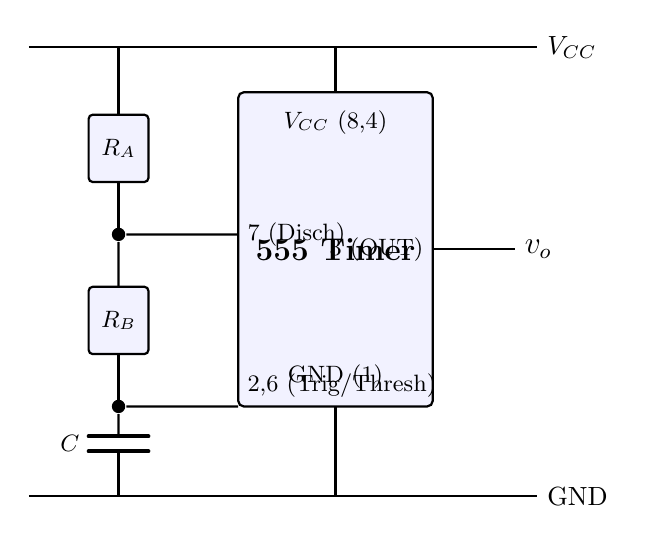
\begin{tikzpicture}[scale=0.95, transform shape]
  % Rails
  \draw[thick] (0, 5.2) -- (6.8, 5.2) node[right] {$V_{CC}$};
  \draw[thick] (0, -0.8) -- (6.8, -0.8) node[right] {GND};

  % Resistors RA and RB
  \draw[thick] (1.2, 5.2) -- (1.2, 4.3);
  \draw[thick, fill=blue!5, rounded corners=1.5pt] (0.8, 3.4) rectangle (1.6, 4.3) node[midway] {\small $R_A$};
  \draw[thick] (1.2, 3.4) -- (1.2, 2.7) node[circle, fill, inner sep=1.8pt] (dis) {};
  \draw[thick] (dis) -- (1.2, 2.0);
  \draw[thick, fill=blue!5, rounded corners=1.5pt] (0.8, 1.1) rectangle (1.6, 2.0) node[midway] {\small $R_B$};
  \draw[thick] (1.2, 1.1) -- (1.2, 0.4) node[circle, fill, inner sep=1.8pt] (trig) {};

  % Timing Capacitor C
  \draw[thick] (trig) -- (1.2, 0.0);
  \draw[line width=1.4pt, line cap=round] (0.8, 0.0) -- (1.6, 0.0);
  \draw[line width=1.4pt, line cap=round] (0.8, -0.2) -- (1.6, -0.2);
  \node[left] at (0.8, -0.1) {\small $C$};
  \draw[thick] (1.2, -0.2) -- (1.2, -0.8);

  % 555 IC Box
  \draw[thick, fill=blue!5, rounded corners=2pt] (2.8, 0.4) rectangle (5.4, 4.6);
  \node at (4.1, 2.5) {\large\textbf{555 Timer}};
  \node at (4.1, 4.2) {\small $V_{CC}$ (8,4)};
  \draw[thick] (4.1, 4.6) -- (4.1, 5.2);
  \node at (4.1, 0.8) {\small GND (1)};
  \draw[thick] (4.1, 0.4) -- (4.1, -0.8);

  % Discharge pin 7
  \draw[thick] (dis) -- (2.8, 2.7);
  \node[right] at (2.8, 2.7) {\small 7 (Disch)};

  % Trigger & Threshold pins 2, 6
  \draw[thick] (trig) -- (2.8, 0.4);
  \node[above right] at (2.8, 0.4) {\small 2,6 (Trig/Thresh)};

  % Output Pin 3
  \draw[thick] (5.4, 2.5) -- (6.5, 2.5) node[right] {\large $v_o$};
  \node[left] at (5.4, 2.5) {\small 3 (OUT)};
\end{tikzpicture}
\end{schematicbox}

\begin{enumerate}[leftmargin=1.5em]
  \item \textbf{Charging Time ($T_{\text{HIGH}}$):}
  \[
  v_C(t) = V_{CC} - \frac{2}{3}V_{CC} e^{-t / (R_A+R_B)C} = \frac{2}{3}V_{CC} \implies T_{\text{HIGH}} = (R_A + R_B) C \ln(2) \approx \mathbf{0.693(R_A + R_B)C}
  \]
  \item \textbf{Discharging Time ($T_{\text{LOW}}$):}
  \[
  v_C(t) = \frac{2}{3}V_{CC} e^{-t / R_B C} = \frac{1}{3}V_{CC} \implies T_{\text{LOW}} = R_B C \ln(2) \approx \mathbf{0.693 R_B C}
  \]
  \item \textbf{Total Period and Frequency:}
  \[
  T = T_{\text{HIGH}} + T_{\text{LOW}} = 0.693(R_A + 2R_B)C \implies \mathbf{f = \frac{1}{T} = \frac{1.44}{(R_A + 2R_B)C}}
  \]
\end{enumerate}

\begin{answerbox}
$$\mathbf{f = \frac{1.44}{(R_A + 2R_B)C}, \qquad \text{Duty Cycle } D = \frac{R_A + R_B}{R_A + 2R_B} \times 100\%}$$
\end{answerbox}

\vspace{0.6cm}

% =========================================================================
% QUESTION 12
% =========================================================================
\subsection{Question 12: Series Voltage Regulator with Current Limiting \& LM317 Design [4 + 4 = 8 Marks]}
\begin{questionbox}{Problem Statement (2082 Baishakh, Q12)}
Draw series voltage regulator with current limiting circuit and explain how this protection circuit works. Design a voltage regulator to give output voltage from $5\text{V}$ to $15\text{V}$ using LM317.
\end{questionbox}

\paragraph{Part (a): Current Limiting Protection Circuit [4 Marks]}
\begin{schematicbox}{Series Transistor Voltage Regulator with Current Limiting Protection}
\centering
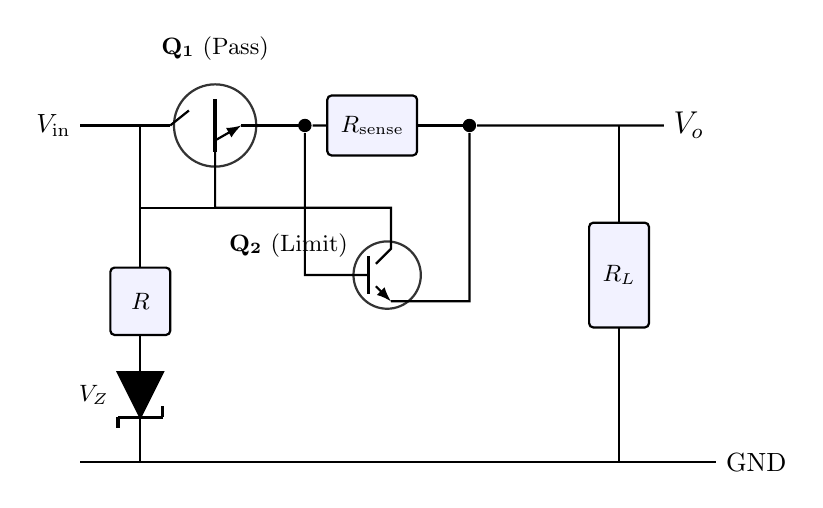
\begin{tikzpicture}[scale=0.95, transform shape]
  % Rails
  \draw[thick] (0, 4.5) node[left] {$V_{\text{in}}$} -- (1.2, 4.5);
  \draw[thick] (0, 0) -- (8.5, 0) node[right] {GND};

  % Pass Transistor Q1 (NPN)
  \draw[draw=black!80, fill=white, thick] (1.8, 4.5) circle (0.55cm);
  \draw[line width=1.6pt] (1.8, 4.15) -- (1.8, 4.85); % Base
  \draw[thick] (1.2, 4.5) -- (1.45, 4.7); % Collector
  \draw[thick, ->, >=latex] (1.8, 4.3) -- (2.15, 4.5); % Emitter
  \draw[thick] (2.15, 4.5) -- (3.0, 4.5) node[circle, fill, inner sep=1.8pt] (n_sense) {};
  \node[above=0.2cm] at (1.8, 5.05) {\small $\mathbf{Q_1}$ (Pass)};

  % Current Sensing Resistor R_sense
  \draw[thick] (n_sense) -- (3.3, 4.5);
  \draw[thick, fill=blue!5, rounded corners=1.5pt] (3.3, 4.1) rectangle (4.5, 4.9) node[midway] {\small $R_{\text{sense}}$};
  \draw[thick] (4.5, 4.5) -- (5.2, 4.5) node[circle, fill, inner sep=1.8pt] (n_out) {};
  \draw[thick] (n_out) -- (7.8, 4.5) node[right] {\large $V_o$};

  % Current Limiting Transistor Q2 (NPN)
  \draw[draw=black!80, fill=white, thick] (4.1, 2.5) circle (0.45cm);
  \draw[line width=1.4pt] (3.85, 2.25) -- (3.85, 2.75); % Base
  \draw[thick] (n_sense) -- (3.0, 2.5) -- (3.85, 2.5); % Base connected before Rsense
  \draw[thick, ->, >=latex] (3.95, 2.35) -- (4.15, 2.15); % Emitter
  \draw[thick] (4.15, 2.15) -- (5.2, 2.15) -- (n_out); % Emitter connected after Rsense
  \draw[thick] (3.95, 2.65) -- (4.15, 2.85) -- (4.15, 3.4) -- (1.8, 3.4) -- (1.8, 4.15); % Collector pulls down Q1 base
  \node[left=0.15cm] at (3.85, 2.9) {\small $\mathbf{Q_2}$ (Limit)};

  % Base bias resistor and Zener
  \draw[thick] (0.8, 4.5) -- (0.8, 3.4) -- (1.8, 3.4);
  \draw[thick] (0.8, 3.4) -- (0.8, 2.6);
  \draw[thick, fill=blue!5, rounded corners=1.5pt] (0.4, 1.7) rectangle (1.2, 2.6) node[midway] {\small $R$};
  \draw[thick] (0.8, 1.7) -- (0.8, 1.2);
  % Zener
  \draw[thick, fill=black] (0.5, 1.2) -- (1.1, 1.2) -- (0.8, 0.6) -- cycle;
  \draw[line width=1.2pt] (0.5, 0.6) -- (1.1, 0.6);
  \draw[line width=1.2pt] (0.5, 0.6) -- (0.5, 0.45);
  \draw[line width=1.2pt] (1.1, 0.6) -- (1.1, 0.75);
  \node[left] at (0.5, 0.9) {\small $V_Z$};
  \draw[thick] (0.8, 0.6) -- (0.8, 0);

  % Load Resistor
  \draw[thick] (7.2, 4.5) -- (7.2, 3.2);
  \draw[thick, fill=blue!5, rounded corners=1.5pt] (6.8, 1.8) rectangle (7.6, 3.2) node[midway] {\small $R_L$};
  \draw[thick] (7.2, 1.8) -- (7.2, 0);
\end{tikzpicture}
\end{schematicbox}

\paragraph{Circuit Operation:}
A current-sense resistor $R_{\text{sense}}$ and protection transistor $Q_2$ are placed in series with pass transistor $Q_1$:
\begin{itemize}[leftmargin=1.5em]
  \item \textbf{Normal Operation ($I_L < I_{\text{limit}}$):} The voltage drop across $R_{\text{sense}}$ is less than the cut-in voltage ($I_L R_{\text{sense}} < 0.6\text{V}$). Transistor $Q_2$ is OFF and does not interfere with regular voltage regulation.
  \item \textbf{Overload / Short-Circuit Condition ($I_L \ge I_{\text{limit}}$):}
  When $I_L R_{\text{sense}} \ge 0.7\text{V}$, transistor $Q_2$ turns ON, diverting excess base drive current away from pass transistor $Q_1$. This limits the maximum output current to a safe threshold:
  \[
  \mathbf{I_{\text{limit}} = \frac{V_{BE2}}{R_{\text{sense}}} \approx \frac{0.7\text{V}}{R_{\text{sense}}}}
  \]
\end{itemize}

\paragraph{Part (b): LM317 Design for $5\text{V} - 15\text{V}$ Output [4 Marks]}
\[
V_{\text{out}} = 1.25\text{V} \left(1 + \frac{R_2}{R_1}\right)
\]
\begin{enumerate}[leftmargin=1.5em]
  \item Select standard $R_1 = \mathbf{240\ \Omega}$.
  \item For $V_{\text{out}(\min)} = 5.0\text{V}$:
  \[
  5.0 = 1.25 \left(1 + \frac{R_{2(\min)}}{240}\right) \implies 1 + \frac{R_{2(\min)}}{240} = 4.0 \implies R_{2(\min)} = 3 \times 240 = \mathbf{720\ \Omega}
  \]
  \item For $V_{\text{out}(\max)} = 15.0\text{V}$:
  \[
  15.0 = 1.25 \left(1 + \frac{R_{2(\max)}}{240}\right) \implies 1 + \frac{R_{2(\max)}}{240} = 12.0 \implies R_{2(\max)} = 11 \times 240 = \mathbf{2640\ \Omega} = \mathbf{2.64\text{ k}\Omega}
  \]
\end{enumerate}
\textbf{Implementation:} Use a fixed resistor $R_{2A} = 680\ \Omega$ in series with a $\mathbf{2.0\text{ k}\Omega}$ linear potentiometer.

\begin{answerbox}
$$\mathbf{R_1 = 240\ \Omega, \qquad R_2 = 720\ \Omega \text{ to } 2.64\text{ k}\Omega \quad (\text{Fixed } 680\ \Omega + 2.0\text{k}\Omega \text{ Potentiometer})}$$
\end{answerbox}

\chapter{2081 Ashwin Examination Solutions}

\section*{Examination Overview}
\begin{tabular}{@{}ll@{}}
\textbf{Level:} Bachelor in Engineering (BE) & \textbf{Full Marks:} 60 \\
\textbf{Programme:} BEI, BCT & \textbf{Pass Marks:} 24 \\
\textbf{Year / Part:} I / II & \textbf{Time:} 3 Hours \\
\textbf{Subject:} Electronic Devices \& Circuits (EX 151) & \textbf{Examination Type:} Regular (New Course - 2080 Batch) \\
\end{tabular}

\vspace{0.6cm}
\hrule
\vspace{0.6cm}

% =========================================================================
% QUESTION 1
% =========================================================================
\subsection{Question 1: Stiff $\beta$-Independent CE Amplifier Design [4 Marks]}
\begin{questionbox}{Problem Statement (2081 Ashwin, Q1)}
Design $\beta$-independent type DC biased common emitter amplifier. Given parameters: $V_{CC} = 20\text{V}, I_C = 1.5\text{mA}$ and $\beta = 110$. Use stiff biasing method.
\end{questionbox}

\begin{enumerate}[leftmargin=1.5em]
  \item \textbf{Emitter Voltage Allocation ($V_E$):}
  Set $V_E = 0.10 \times V_{CC} = 0.10 \times 20\text{V} = \mathbf{2.0\text{V}}$.
  \[
  R_E = \frac{V_E}{I_E} \approx \frac{2.0\text{V}}{1.5\text{mA}} = 1.33\text{ k}\Omega \quad (\text{Select standard } R_E = \mathbf{1.3\text{ k}\Omega}\text{ or } \mathbf{1.5\text{ k}\Omega})
  \]
  \item \textbf{Collector Resistor Allocation ($R_C$):}
  Set $V_{CEQ} = \frac{V_{CC} - V_E}{2} = \frac{20 - 2.0}{2} = 9.0\text{V}$:
  \[
  R_C = \frac{V_{CC} - (V_E + V_{CEQ})}{I_C} = \frac{20 - 11.0}{1.5\text{mA}} = \frac{9.0\text{V}}{1.5\text{mA}} = \mathbf{6.0\text{ k}\Omega} \quad (\text{Select standard } R_C = \mathbf{6.2\text{ k}\Omega})
  \]
  \item \textbf{Base Voltage Calculation ($V_B$):}
  \[
  V_B = V_E + V_{BE} = 2.0\text{V} + 0.7\text{V} = \mathbf{2.7\text{ V}}
  \]
  \item \textbf{Stiff Biasing Bleeder Current Rule ($I_{\text{bleed}} \ge 10 I_B$):}
  \[
  I_B = \frac{1.5\text{mA}}{110} = 13.64\ \mu\text{A} \implies I_{\text{bleed}} = 10 \times 13.64\ \mu\text{A} = 136.4\ \mu\text{A} = 0.1364\text{mA}
  \]
  \[
  R_2 = \frac{V_B}{I_{\text{bleed}}} = \frac{2.7\text{V}}{0.1364\text{mA}} = 19.79\text{ k}\Omega \quad (\text{Select standard } R_2 = \mathbf{20\text{ k}\Omega}\text{ or } \mathbf{18\text{ k}\Omega})
  \]
  \[
  R_1 = \frac{V_{CC} - V_B}{I_{\text{bleed}} + I_B} = \frac{20\text{V} - 2.7\text{V}}{0.15\text{mA}} = \frac{17.3\text{V}}{0.15\text{mA}} = 115.33\text{ k}\Omega \quad (\text{Select standard } R_1 = \mathbf{120\text{ k}\Omega})
  \]
\end{enumerate}

\begin{schematicbox}{Designed Stiff CE Amplifier Circuit ($V_{CC} = 20\text{V}$)}
\centering
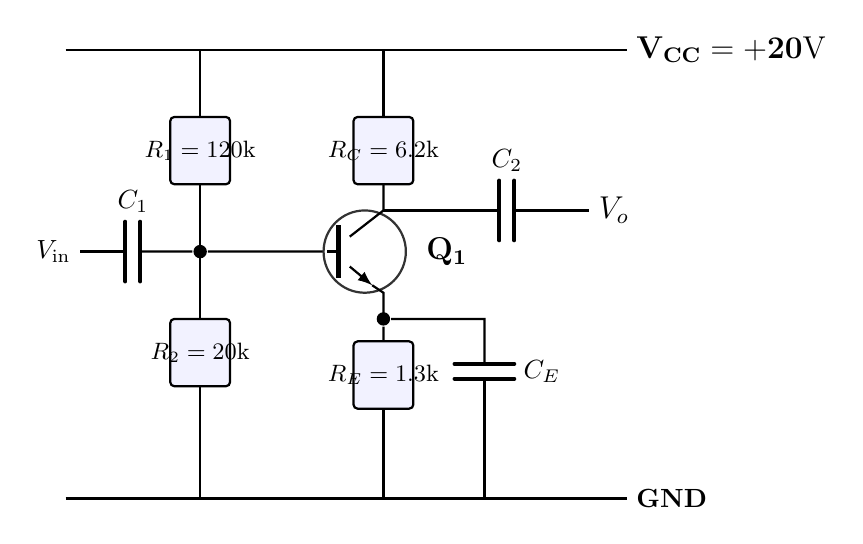
\begin{tikzpicture}[scale=0.95, transform shape]
  % Rails
  \draw[thick] (0, 5.2) -- (7.5, 5.2) node[right] {\large $\mathbf{V_{CC} = +20\text{V}}$};
  \draw[thick] (0, -0.8) -- (7.5, -0.8) node[right] {\textbf{GND}};

  % Divider R1 and R2
  \draw[thick] (1.8, 5.2) -- (1.8, 4.3);
  \draw[thick, fill=blue!5, rounded corners=1.5pt] (1.4, 3.4) rectangle (2.2, 4.3) node[midway] {\small $R_1=120\text{k}$};
  \draw[thick] (1.8, 3.4) -- (1.8, 2.5) node[circle, fill, inner sep=1.8pt] (vb) {};
  \draw[thick] (1.8, 2.5) -- (1.8, 1.6);
  \draw[thick, fill=blue!5, rounded corners=1.5pt] (1.4, 0.7) rectangle (2.2, 1.6) node[midway] {\small $R_2=20\text{k}$};
  \draw[thick] (1.8, 0.7) -- (1.8, -0.8);

  % Input coupling capacitor C1
  \draw[thick] (0.2, 2.5) node[left] {$V_{\text{in}}$} -- (0.8, 2.5);
  \draw[line width=1.4pt, line cap=round] (0.8, 2.1) -- (0.8, 2.9);
  \draw[line width=1.4pt, line cap=round] (1.0, 2.1) -- (1.0, 2.9);
  \node[above] at (0.9, 2.9) {$C_1$};
  \draw[thick] (1.0, 2.5) -- (vb);

  % Transistor Q1 (NPN)
  \draw[thick] (vb) -- (3.5, 2.5);
  \draw[draw=black!80, fill=white, thick] (4.0, 2.5) circle (0.55cm);
  \draw[line width=1.6pt] (3.65, 2.15) -- (3.65, 2.85); % Base
  \draw[thick] (3.5, 2.5) -- (3.65, 2.5);
  \draw[thick] (3.8, 2.7) -- (4.25, 3.05) -- (4.25, 3.4); % Collector
  \draw[thick, ->, >=latex] (3.8, 2.3) -- (4.1, 2.05); % Emitter
  \draw[thick] (4.1, 2.05) -- (4.25, 1.95) -- (4.25, 1.6) node[circle, fill, inner sep=1.8pt] (ve) {};
  \node[right=0.2cm] at (4.5, 2.5) {\large $\mathbf{Q_1}$};

  % Collector Resistor RC
  \draw[thick, fill=blue!5, rounded corners=1.5pt] (3.85, 3.4) rectangle (4.65, 4.3) node[midway] {\small $R_C=6.2\text{k}$};
  \draw[thick] (4.25, 4.3) -- (4.25, 5.2);

  % Emitter Resistor RE and Bypass CE
  \draw[thick] (ve) -- (4.25, 1.3);
  \draw[thick, fill=blue!5, rounded corners=1.5pt] (3.85, 0.4) rectangle (4.65, 1.3) node[midway] {\small $R_E=1.3\text{k}$};
  \draw[thick] (4.25, 0.4) -- (4.25, -0.8);

  % Bypass Capacitor CE
  \draw[thick] (ve) -- (5.6, 1.6) -- (5.6, 1.0);
  \draw[line width=1.4pt, line cap=round] (5.2, 1.0) -- (6.0, 1.0);
  \draw[line width=1.4pt, line cap=round] (5.2, 0.8) -- (6.0, 0.8);
  \node[right] at (6.0, 0.9) {$C_E$};
  \draw[thick] (5.6, 0.8) -- (5.6, -0.8);

  % Output coupling capacitor C2
  \draw[thick] (4.25, 3.05) -- (5.8, 3.05);
  \draw[line width=1.4pt, line cap=round] (5.8, 2.65) -- (5.8, 3.45);
  \draw[line width=1.4pt, line cap=round] (6.0, 2.65) -- (6.0, 3.45);
  \node[above] at (5.9, 3.45) {$C_2$};
  \draw[thick] (6.0, 3.05) -- (7.0, 3.05) node[right] {\large $V_o$};
\end{tikzpicture}
\end{schematicbox}

\begin{answerbox}
$$\mathbf{R_1 = 120\text{ k}\Omega, \quad R_2 = 20\text{ k}\Omega, \quad R_C = 6.2\text{ k}\Omega, \quad R_E = 1.3\text{ k}\Omega}$$
\end{answerbox}

\vspace{0.6cm}

% =========================================================================
% QUESTION 2
% =========================================================================
\subsection{Question 2: Common Collector (Emitter Follower) Small Signal Analysis [1 + 4 = 5 Marks]}
\begin{questionbox}{Problem Statement (2081 Ashwin, Q2)}
Why is a common collector BJT amplifier also known as an emitter follower? Draw the small signal model of common collector amplifier circuit and derive expressions for input resistance, voltage gain, and current gain.
\end{questionbox}

\paragraph{Part (a): Why Termed "Emitter Follower" [1 Mark]}
In a Common Collector configuration, the output voltage is extracted at the emitter terminal. Since $v_o = v_e = v_{\text{in}} - v_{be} \approx v_{\text{in}}$ and the voltage gain is nearly unity ($A_v \approx 0.99 \approx 1$) with zero phase shift ($0^\circ$), the emitter AC output potential \textbf{closely tracks and follows the input signal}, hence the name \textbf{Emitter Follower}.

\paragraph{Part (b): Parameter Derivations [4 Marks]}
\begin{schematicbox}{Small-Signal Model of Common Collector (Emitter Follower)}
\centering
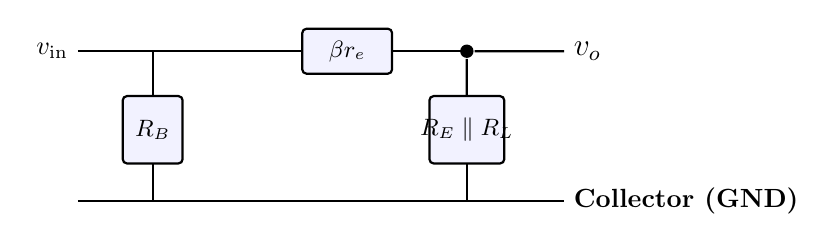
\begin{tikzpicture}[scale=0.95, transform shape]
  % Input
  \draw[thick] (0, 2.0) node[left] {$v_{\text{in}}$} -- (1.5, 2.0);
  % RB
  \draw[thick] (1.0, 2.0) -- (1.0, 1.4);
  \draw[thick, fill=blue!5, rounded corners=1.5pt] (0.6, 0.5) rectangle (1.4, 1.4) node[midway] {\small $R_B$};
  \draw[thick] (1.0, 0.5) -- (1.0, 0);

  % Base to Emitter branch: beta*re and (1+beta)*(RE || RL)
  \draw[thick] (1.5, 2.0) -- (3.0, 2.0);
  \draw[thick, fill=blue!5, rounded corners=1.5pt] (3.0, 1.7) rectangle (4.2, 2.3) node[midway] {\small $\beta r_e$};
  \draw[thick] (4.2, 2.0) -- (5.2, 2.0) node[circle, fill, inner sep=1.8pt] (ve) {};

  % RE || RL
  \draw[thick] (ve) -- (5.2, 1.4);
  \draw[thick, fill=blue!5, rounded corners=1.5pt] (4.7, 0.5) rectangle (5.7, 1.4) node[midway] {\small $R_E \parallel R_L$};
  \draw[thick] (5.2, 0.5) -- (5.2, 0);

  % Ground Rail
  \draw[thick] (0, 0) -- (6.5, 0) node[right] {\textbf{Collector (GND)}};

  % Output node
  \draw[thick] (ve) -- (6.5, 2.0) node[right] {\large $v_o$};
\end{tikzpicture}
\end{schematicbox}

\begin{enumerate}[leftmargin=1.5em]
  \item \textbf{Input Resistance ($R_{\text{in}}$):}
  Looking into the base terminal:
  \[
  Z_b = \beta r_e + (1+\beta)(R_E \parallel R_L) \approx \mathbf{\beta (r_e + R_E \parallel R_L)} \quad (\text{very high, } > 100\text{ k}\Omega)
  \]
  Total amplifier input resistance: $R_{\text{in}} = R_1 \parallel R_2 \parallel Z_b$.
  \item \textbf{Voltage Gain ($A_v$):}
  \[
  v_o = i_e (R_E \parallel R_L), \qquad v_{\text{in}} = i_e [r_e + (R_E \parallel R_L)]
  \]
  \[
  \mathbf{A_v = \frac{v_o}{v_{\text{in}}} = \frac{R_E \parallel R_L}{r_e + R_E \parallel R_L} \approx 1 \quad (\text{Non-inverting, } 0^\circ \text{ phase shift})}
  \]
  \item \textbf{Current Gain ($A_i$):}
  \[
  \mathbf{A_i = \frac{i_o}{i_{\text{in}}} = (1+\beta) \left(\frac{R_B}{R_B + Z_b}\right) \left(\frac{R_E}{R_E + R_L}\right) \approx \beta} \quad (\text{very high})
  \]
\end{enumerate}

\begin{answerbox}
$$\mathbf{R_{\text{in}} \approx R_B \parallel \beta R_E, \qquad A_v = \frac{R_E \parallel R_L}{r_e + R_E \parallel R_L} \approx 1, \qquad A_i \approx \beta}$$
\end{answerbox}

\vspace{0.6cm}

% =========================================================================
% QUESTION 3
% =========================================================================
\subsection{Question 3: Derivation of BJT Transconductance $g_m$ [4 Marks]}
\begin{questionbox}{Problem Statement (2081 Ashwin, Q3)}
Derive trans-conductance of BJT.
\end{questionbox}

The transconductance $g_m$ quantifies the small-signal sensitivity of the collector output current with respect to changes in the base-emitter input voltage:
\[
g_m = \left. \frac{\partial i_C}{\partial v_{BE}} \right|_{Q-\text{point}}
\]
\paragraph{Derivation from Shockley Diode Conduction Equation:}
The collector current of a BJT operating in the active region is given by:
\[
i_C = I_S e^{v_{BE} / V_T}
\]
where $I_S$ is the reverse saturation current and $V_T = \frac{kT}{q} \approx 26\text{ mV}$ is the thermal voltage at room temperature ($300\text{ K}$).\\
Differentiating with respect to $v_{BE}$:
\[
\frac{d i_C}{d v_{BE}} = I_S \cdot \frac{d}{d v_{BE}}\left(e^{v_{BE}/V_T}\right) = I_S \cdot \left(\frac{1}{V_T} e^{v_{BE}/V_T}\right) = \frac{I_S e^{v_{BE}/V_T}}{V_T}
\]
Recognizing that $I_S e^{V_{BEQ}/V_T} = I_C$ (quiescent collector current):
\[
\mathbf{g_m = \frac{I_C}{V_T} = \frac{1}{r_e}} \quad \blacksquare
\]

\begin{answerbox}
$$\mathbf{g_m = \frac{I_C}{V_T} \approx \frac{I_C}{26\text{ mV}}}$$
\end{answerbox}

\vspace{0.6cm}

% =========================================================================
% QUESTION 4
% =========================================================================
\subsection{Question 4: N-Channel Enhancement-Type MOSFET [7 Marks]}
\begin{questionbox}{Problem Statement (2081 Ashwin, Q4)}
Describe the construction and working principle of n channel enhancement-type MOSFET with the help of necessary diagrams and its drain characteristic curve.
\end{questionbox}

\paragraph{1. Physical Construction:}
An N-Channel Enhancement MOSFET (E-MOSFET) is fabricated on a p-type substrate without any pre-existing channel:
\begin{itemize}[leftmargin=1.5em]
  \item Two heavily doped $n^+$ regions form the Source and Drain.
  \item A thin dielectric insulating layer of $\text{SiO}_2$ separates the metal/polysilicon Gate electrode from the substrate.
  \item With $V_{GS} = 0\text{V}$, two back-to-back $p$-$n$ junctions block all current flow between drain and source ($I_D = 0$).
\end{itemize}

\paragraph{2. Working Principle and Inversion Layer Formation:}
\begin{itemize}[leftmargin=1.5em]
  \item When a positive gate voltage is applied ($V_{GS} > 0$), the electric field repels holes away from the surface and attracts minority electrons.
  \item When $V_{GS} \ge V_T$ (\textbf{Threshold Voltage}, typically $+1\text{V}$ to $+3\text{V}$), an \textbf{inversion layer of electrons} forms beneath the gate oxide, creating an induced n-channel bridging source and drain.
\end{itemize}

\begin{schematicbox}{Drain Characteristic Curves of N-Channel E-MOSFET}
\centering
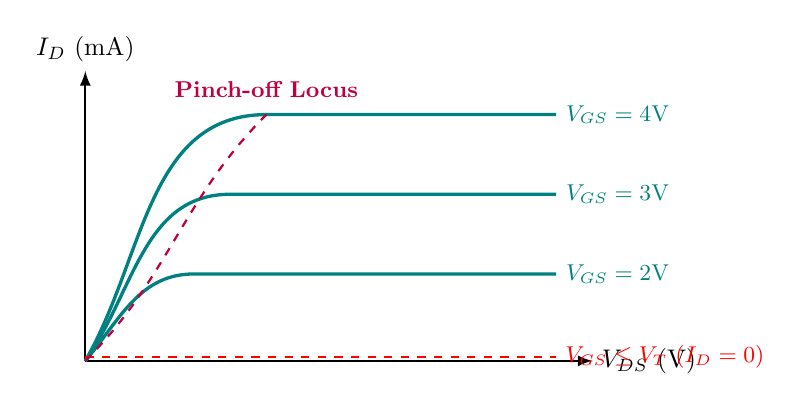
\begin{tikzpicture}[scale=0.92, transform shape]
  \draw[thick, ->, >=latex] (0, 0) -- (7.0, 0) node[right] {$V_{DS}\ (\text{V})$};
  \draw[thick, ->, >=latex] (0, 0) -- (0, 4.0) node[above] {$I_D\ (\text{mA})$};

  \draw[line width=1.2pt, teal] (0, 0) to[out=60, in=180] (2.5, 3.4) -- (6.5, 3.4) node[right] {\small $V_{GS} = 4\text{V}$};
  \draw[line width=1.2pt, teal] (0, 0) to[out=55, in=180] (2.0, 2.3) -- (6.5, 2.3) node[right] {\small $V_{GS} = 3\text{V}$};
  \draw[line width=1.2pt, teal] (0, 0) to[out=50, in=180] (1.5, 1.2) -- (6.5, 1.2) node[right] {\small $V_{GS} = 2\text{V}$};
  \draw[thick, red, dashed] (0, 0.05) -- (6.5, 0.05) node[right] {\small $V_{GS} \le V_T\ (I_D=0)$};
  \draw[thick, dashed, purple] (0, 0) to[out=45, in=-135] (2.5, 3.4) node[above=0.1cm] {\small\textbf{Pinch-off Locus}};
\end{tikzpicture}
\end{schematicbox}

\paragraph{3. Drain Current Conduction Equations:}
\begin{itemize}[leftmargin=1.5em]
  \item \textbf{Ohmic / Triode Region ($V_{DS} < V_{GS} - V_T$):}
  \[
  I_D = K \left[2(V_{GS} - V_T)V_{DS} - V_{DS}^2\right]
  \]
  \item \textbf{Saturation Region ($V_{DS} \ge V_{GS} - V_T$):}
  \[
  \mathbf{I_D = K (V_{GS} - V_T)^2 = \frac{1}{2}\mu_n C_{ox} \left(\frac{W}{L}\right)(V_{GS} - V_T)^2}
  \]
\end{itemize}

\begin{answerbox}
$$\mathbf{I_D = K(V_{GS} - V_T)^2 \quad \text{for } V_{GS} \ge V_T \text{ and } V_{DS} \ge V_{GS} - V_T}$$
\end{answerbox}

\vspace{0.6cm}

% =========================================================================
% QUESTION 5
% =========================================================================
\subsection{Question 5: JFET Q-Point and Pinch-Off Region Verification [6 Marks]}
\begin{questionbox}{Problem Statement (2081 Ashwin, Q5)}
Find $I_D$ and $V_{DS}$ for the following circuit. Given data are $V_P = -5.5\text{V}, I_{DSS} = 10\text{mA}$. Assume all capacitors are ideal and check whether the transistor is operating in the pinch-off region or not.
Circuit parameters: $V_{DD} = 20\text{V}, R_1 = 1.5\text{ M}\Omega, R_2 = 330\text{ k}\Omega, R_D = 2.0\text{ k}\Omega, R_S = 1.0\text{ k}\Omega$.
\end{questionbox}

\begin{schematicbox}{Given JFET Circuit Schematic}
\centering
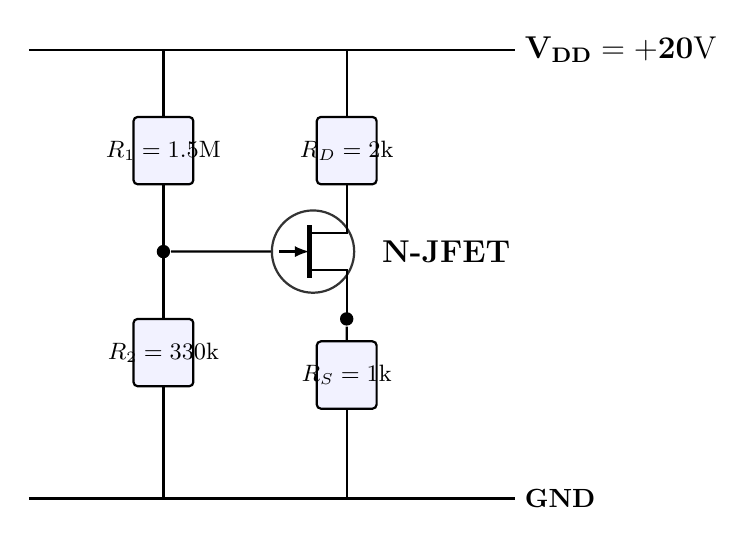
\begin{tikzpicture}[scale=0.95, transform shape]
  % Rails
  \draw[thick] (0, 5.2) -- (6.5, 5.2) node[right] {\large $\mathbf{V_{DD} = +20\text{V}}$};
  \draw[thick] (0, -0.8) -- (6.5, -0.8) node[right] {\textbf{GND}};

  % R1 and R2
  \draw[thick] (1.8, 5.2) -- (1.8, 4.3);
  \draw[thick, fill=blue!5, rounded corners=1.5pt] (1.4, 3.4) rectangle (2.2, 4.3) node[midway] {\small $R_1=1.5\text{M}$};
  \draw[thick] (1.8, 3.4) -- (1.8, 2.5) node[circle, fill, inner sep=1.8pt] (vg) {};
  \draw[thick] (1.8, 2.5) -- (1.8, 1.6);
  \draw[thick, fill=blue!5, rounded corners=1.5pt] (1.4, 0.7) rectangle (2.2, 1.6) node[midway] {\small $R_2=330\text{k}$};
  \draw[thick] (1.8, 0.7) -- (1.8, -0.8);

  % JFET
  \draw[thick] (vg) -- (3.35, 2.5);
  \draw[draw=black!80, fill=white, thick] (3.8, 2.5) circle (0.55cm);
  \draw[line width=1.6pt] (3.75, 2.15) -- (3.75, 2.85); % Channel
  \draw[thick, ->, >=latex] (3.35, 2.5) -- (3.75, 2.5); % Gate
  \draw[thick] (3.75, 2.75) -- (4.25, 2.75) -- (4.25, 3.4); % Drain
  \draw[thick] (3.75, 2.25) -- (4.25, 2.25) -- (4.25, 1.6) node[circle, fill, inner sep=1.8pt] (vs) {}; % Source
  \node[right=0.2cm] at (4.4, 2.5) {\large\textbf{N-JFET}};

  % RD
  \draw[thick, fill=blue!5, rounded corners=1.5pt] (3.85, 3.4) rectangle (4.65, 4.3) node[midway] {\small $R_D=2\text{k}$};
  \draw[thick] (4.25, 4.3) -- (4.25, 5.2);

  % RS
  \draw[thick] (vs) -- (4.25, 1.3);
  \draw[thick, fill=blue!5, rounded corners=1.5pt] (3.85, 0.4) rectangle (4.65, 1.3) node[midway] {\small $R_S=1\text{k}$};
  \draw[thick] (4.25, 0.4) -- (4.25, -0.8);
\end{tikzpicture}
\end{schematicbox}

\paragraph{1. Gate Voltage Calculation ($V_G$):}
\[
V_G = V_{DD} \left(\frac{R_2}{R_1 + R_2}\right) = 20\text{V} \times \left(\frac{330\text{k}\Omega}{1500\text{k}\Omega + 330\text{k}\Omega}\right) = 20 \times \frac{0.33}{1.83} = \mathbf{3.6066\text{ V}}
\]

\paragraph{2. Equation for $V_{GS}$:}
\[
V_{GS} = V_G - I_D R_S = 3.6066 - 1.0 I_D \quad (\text{with } I_D \text{ in mA})
\]

\paragraph{3. Substitution into Shockley's Equation:}
\[
I_D = 10 \left(1 - \frac{3.6066 - 1.0 I_D}{-5.5}\right)^2 = 10 \left(\frac{5.5 + 3.6066 - I_D}{5.5}\right)^2 = \frac{10}{30.25} (9.1066 - I_D)^2
\]
\[
3.025 I_D = 82.93 - 18.213 I_D + I_D^2 \implies I_D^2 - 21.238 I_D + 82.93 = 0
\]
Solving via quadratic formula:
\[
I_D = \frac{21.238 \pm \sqrt{(21.238)^2 - 4(1)(82.93)}}{2} = \frac{21.238 \pm \sqrt{451.05 - 331.72}}{2} = \frac{21.238 \pm 10.924}{2}
\]
Two mathematical roots:
\begin{itemize}[leftmargin=1.5em]
  \item $I_{D1} = 16.081\text{ mA} \implies V_{GS1} = 3.6066 - 16.081 = -12.47\text{V} < V_P$ (\textbf{Invalid}).
  \item $I_{D2} = \mathbf{5.157\text{ mA}} \implies V_{GS2} = 3.6066 - 5.157 = \mathbf{-1.550\text{ V}}$ (\textbf{Valid}!).
\end{itemize}

\paragraph{4. Calculation of Drain-to-Source Voltage ($V_{DS}$):}
\[
V_{DS} = V_{DD} - I_D(R_D + R_S) = 20\text{V} - 5.157\text{mA} \times (2.0\text{k}\Omega + 1.0\text{k}\Omega) = 20 - 5.157(3.0) = \mathbf{4.529\text{ V}}
\]

\paragraph{5. Verification of Pinch-Off Region:}
The minimum drain-to-source voltage required for pinch-off (saturation) is:
\[
V_{DS(\text{sat})} = V_{GS} - V_P = -1.550\text{V} - (-5.5\text{V}) = \mathbf{3.950\text{ V}}
\]
Since $V_{DS} = 4.529\text{V} \ge V_{DS(\text{sat})} = 3.950\text{V}$, \textbf{the JFET is definitively operating in the pinch-off (saturation) region}.

\begin{answerbox}
$$\mathbf{I_D = 5.157\text{ mA}, \quad V_{GS} = -1.550\text{ V}, \quad V_{DS} = 4.529\text{ V}, \quad V_{DS} > (V_{GS} - V_P) \implies \text{Confirmed in Pinch-off Region!}}$$
\end{answerbox}

\vspace{0.6cm}

% =========================================================================
% QUESTION 6
% =========================================================================
\subsection{Question 6: Colpitts Oscillator Schematic \& Frequency Derivation [4 Marks]}
\begin{questionbox}{Problem Statement (2081 Ashwin, Q6)}
State Barkhausen criterion for sinusoidal oscillation. Draw the circuit diagram of Colpitts oscillator and write its frequency of oscillation.
\end{questionbox}

A \textbf{Colpitts Oscillator} utilizes a capacitive voltage divider composed of two capacitors ($C_1, C_2$) in parallel with an inductor $L$ in its feedback tank.

\begin{schematicbox}{BJT Colpitts Oscillator Circuit}
\centering
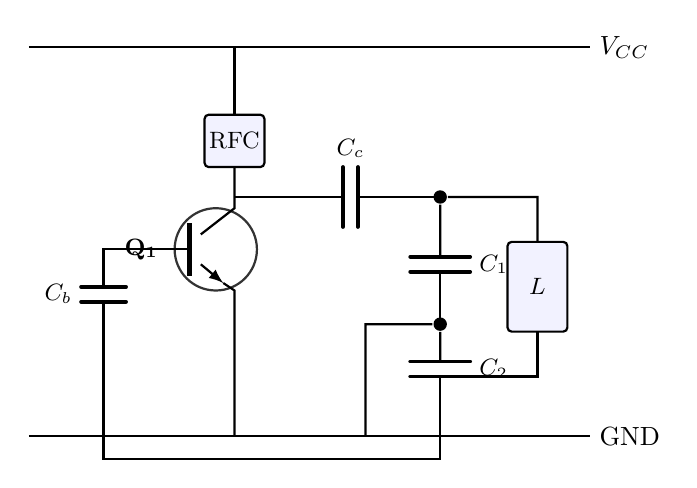
\begin{tikzpicture}[scale=0.95, transform shape]
  % Rails
  \draw[thick] (0, 5.2) -- (7.5, 5.2) node[right] {$V_{CC}$};
  \draw[thick] (0, 0) -- (7.5, 0) node[right] {GND};

  % BJT Transistor Q1 (NPN)
  \draw[draw=black!80, fill=white, thick] (2.5, 2.5) circle (0.55cm);
  \draw[line width=1.6pt] (2.15, 2.15) -- (2.15, 2.85); % Base
  \draw[thick] (2.15, 2.5) -- (1.5, 2.5); % Base lead
  \draw[thick] (2.3, 2.7) -- (2.75, 3.05) -- (2.75, 3.6); % Collector
  \draw[thick, ->, >=latex] (2.3, 2.3) -- (2.6, 2.05); % Emitter
  \draw[thick] (2.6, 2.05) -- (2.75, 1.95) -- (2.75, 0); % Emitter to GND
  \node[left=0.15cm] at (2.0, 2.5) {\small $\mathbf{Q_1}$};

  % Radio Frequency Choke (RFC)
  \draw[thick] (2.75, 3.6) -- (2.75, 4.3);
  \draw[thick, fill=blue!5, rounded corners=1.5pt] (2.35, 3.6) rectangle (3.15, 4.3) node[midway] {\small RFC};
  \draw[thick] (2.75, 4.3) -- (2.75, 5.2);

  % Output to Tank coupling capacitor
  \draw[thick] (2.75, 3.2) -- (4.2, 3.2);
  \draw[line width=1.4pt, line cap=round] (4.2, 2.8) -- (4.2, 3.6);
  \draw[line width=1.4pt, line cap=round] (4.4, 2.8) -- (4.4, 3.6);
  \node[above] at (4.3, 3.6) {\small $C_c$};
  \draw[thick] (4.4, 3.2) -- (5.5, 3.2) node[circle, fill, inner sep=1.8pt] (tank_top) {};

  % Tank Inductor L
  \draw[thick] (tank_top) -- (6.8, 3.2) -- (6.8, 2.6);
  \draw[thick, fill=blue!5, rounded corners=1.5pt] (6.4, 1.4) rectangle (7.2, 2.6) node[midway] {\small $L$};
  \draw[thick] (6.8, 1.4) -- (6.8, 0.8) -- (5.5, 0.8);

  % Split Capacitors C1 and C2
  \draw[thick] (tank_top) -- (5.5, 2.4);
  \draw[line width=1.4pt, line cap=round] (5.1, 2.4) -- (5.9, 2.4);
  \draw[line width=1.4pt, line cap=round] (5.1, 2.2) -- (5.9, 2.2);
  \node[right] at (5.9, 2.3) {\small $C_1$};
  \draw[thick] (5.5, 2.2) -- (5.5, 1.5) node[circle, fill, inner sep=1.8pt] (tap) {};
  \draw[thick] (tap) -- (4.5, 1.5) -- (4.5, 0); % Grounded center tap

  \draw[thick] (tap) -- (5.5, 1.0);
  \draw[line width=1.4pt, line cap=round] (5.1, 1.0) -- (5.9, 1.0);
  \draw[line width=1.4pt, line cap=round] (5.1, 0.8) -- (5.9, 0.8);
  \node[right] at (5.9, 0.9) {\small $C_2$};
  \draw[thick] (5.5, 0.8) -- (5.5, -0.3) -- (1.0, -0.3) -- (1.0, 1.8);
  \draw[line width=1.4pt, line cap=round] (0.7, 1.8) -- (1.3, 1.8);
  \draw[line width=1.4pt, line cap=round] (0.7, 2.0) -- (1.3, 2.0);
  \node[left] at (0.7, 1.9) {\small $C_b$};
  \draw[thick] (1.0, 2.0) -- (1.0, 2.5) -- (1.5, 2.5); % Feedback to base
\end{tikzpicture}
\end{schematicbox}

\paragraph{Frequency of Oscillation:}
The series combination of $C_1$ and $C_2$ gives the equivalent tank capacitance:
\[
C_{\text{eq}} = \frac{C_1 C_2}{C_1 + C_2} \implies \mathbf{f_0 = \frac{1}{2\pi \sqrt{L C_{\text{eq}}}} = \frac{1}{2\pi \sqrt{L \left(\frac{C_1 C_2}{C_1 + C_2}\right)}}}
\]

\begin{answerbox}
$$\mathbf{f_0 = \frac{1}{2\pi \sqrt{L C_{\text{eq}}}}, \qquad C_{\text{eq}} = \frac{C_1 C_2}{C_1 + C_2}}$$
\end{answerbox}

\vspace{0.6cm}

% =========================================================================
% QUESTION 7
% =========================================================================
\subsection{Question 7: 555 Timer Astable Multivibrator Frequency Derivation [4 Marks]}
\begin{questionbox}{Problem Statement (2081 Ashwin, Q7)}
Derive frequency of oscillation of 555 timer Astable Multivibrator.
\end{questionbox}

\begin{schematicbox}{555 Timer Astable Multivibrator Circuit}
\centering
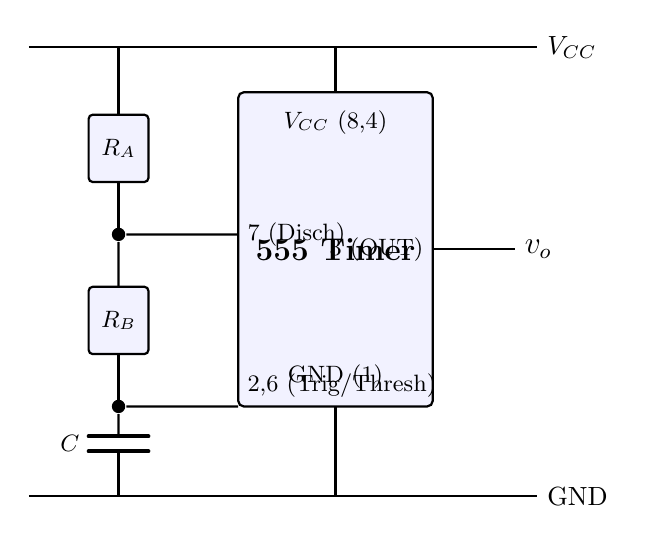
\begin{tikzpicture}[scale=0.95, transform shape]
  % Rails
  \draw[thick] (0, 5.2) -- (6.8, 5.2) node[right] {$V_{CC}$};
  \draw[thick] (0, -0.8) -- (6.8, -0.8) node[right] {GND};

  % Resistors RA and RB
  \draw[thick] (1.2, 5.2) -- (1.2, 4.3);
  \draw[thick, fill=blue!5, rounded corners=1.5pt] (0.8, 3.4) rectangle (1.6, 4.3) node[midway] {\small $R_A$};
  \draw[thick] (1.2, 3.4) -- (1.2, 2.7) node[circle, fill, inner sep=1.8pt] (dis) {};
  \draw[thick] (dis) -- (1.2, 2.0);
  \draw[thick, fill=blue!5, rounded corners=1.5pt] (0.8, 1.1) rectangle (1.6, 2.0) node[midway] {\small $R_B$};
  \draw[thick] (1.2, 1.1) -- (1.2, 0.4) node[circle, fill, inner sep=1.8pt] (trig) {};

  % Timing Capacitor C
  \draw[thick] (trig) -- (1.2, 0.0);
  \draw[line width=1.4pt, line cap=round] (0.8, 0.0) -- (1.6, 0.0);
  \draw[line width=1.4pt, line cap=round] (0.8, -0.2) -- (1.6, -0.2);
  \node[left] at (0.8, -0.1) {\small $C$};
  \draw[thick] (1.2, -0.2) -- (1.2, -0.8);

  % 555 IC Box
  \draw[thick, fill=blue!5, rounded corners=2pt] (2.8, 0.4) rectangle (5.4, 4.6);
  \node at (4.1, 2.5) {\large\textbf{555 Timer}};
  \node at (4.1, 4.2) {\small $V_{CC}$ (8,4)};
  \draw[thick] (4.1, 4.6) -- (4.1, 5.2);
  \node at (4.1, 0.8) {\small GND (1)};
  \draw[thick] (4.1, 0.4) -- (4.1, -0.8);

  % Discharge pin 7
  \draw[thick] (dis) -- (2.8, 2.7);
  \node[right] at (2.8, 2.7) {\small 7 (Disch)};

  % Trigger & Threshold pins 2, 6
  \draw[thick] (trig) -- (2.8, 0.4);
  \node[above right] at (2.8, 0.4) {\small 2,6 (Trig/Thresh)};

  % Output Pin 3
  \draw[thick] (5.4, 2.5) -- (6.5, 2.5) node[right] {\large $v_o$};
  \node[left] at (5.4, 2.5) {\small 3 (OUT)};
\end{tikzpicture}
\end{schematicbox}

\begin{enumerate}[leftmargin=1.5em]
  \item \textbf{Charging Time ($T_{\text{HIGH}}$):}
  \[
  v_C(t) = V_{CC} - \frac{2}{3}V_{CC} e^{-t / (R_A+R_B)C} = \frac{2}{3}V_{CC} \implies T_{\text{HIGH}} = (R_A + R_B) C \ln(2) \approx \mathbf{0.693(R_A + R_B)C}
  \]
  \item \textbf{Discharging Time ($T_{\text{LOW}}$):}
  \[
  v_C(t) = \frac{2}{3}V_{CC} e^{-t / R_B C} = \frac{1}{3}V_{CC} \implies T_{\text{LOW}} = R_B C \ln(2) \approx \mathbf{0.693 R_B C}
  \]
  \item \textbf{Total Period and Frequency:}
  \[
  T = T_{\text{HIGH}} + T_{\text{LOW}} = 0.693(R_A + 2R_B)C \implies \mathbf{f = \frac{1}{T} = \frac{1.44}{(R_A + 2R_B)C}}
  \]
\end{enumerate}

\begin{answerbox}
$$\mathbf{f = \frac{1.44}{(R_A + 2R_B)C}, \qquad T_{\text{HIGH}} = 0.693(R_A+R_B)C, \qquad T_{\text{LOW}} = 0.693 R_B C}$$
\end{answerbox}

\vspace{0.6cm}

% =========================================================================
% QUESTION 8
% =========================================================================
\subsection{Question 8: Widlar Current Source Output Resistance Derivation [5 Marks]}
\begin{questionbox}{Problem Statement (2081 Ashwin, Q8)}
Draw a Widlar Current Source. Derive an expression for an output resistance of Widlar Current Source.
\end{questionbox}

\begin{schematicbox}{Widlar Current Source Circuit Diagram}
\centering
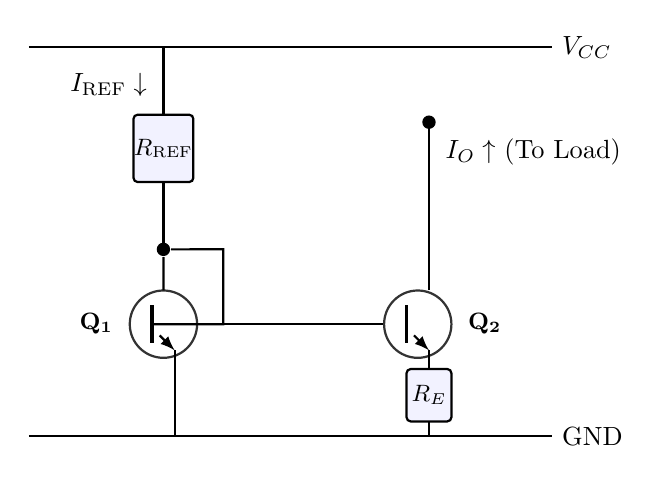
\begin{tikzpicture}[scale=0.95, transform shape]
  % Rails
  \draw[thick] (0, 5.2) -- (7.0, 5.2) node[right] {$V_{CC}$};
  \draw[thick] (0, 0) -- (7.0, 0) node[right] {GND};

  % Reference resistor R_REF
  \draw[thick] (1.8, 5.2) -- (1.8, 4.3);
  \draw[thick, fill=blue!5, rounded corners=1.5pt] (1.4, 3.4) rectangle (2.2, 4.3) node[midway] {\small $R_{\text{REF}}$};
  \draw[thick] (1.8, 3.4) -- (1.8, 2.5) node[circle, fill, inner sep=1.8pt] (n1) {};
  \node[left=0.1cm] at (1.8, 4.7) {$I_{\text{REF}} \downarrow$};

  % Transistor Q1 (Diode connected NPN)
  \draw[draw=black!80, fill=white, thick] (1.8, 1.5) circle (0.45cm);
  \draw[line width=1.4pt] (1.65, 1.25) -- (1.65, 1.75); % Base
  \draw[thick] (n1) -- (1.8, 1.95); % Collector
  \draw[thick, ->, >=latex] (1.75, 1.35) -- (1.95, 1.15); % Emitter
  \draw[thick] (1.95, 1.15) -- (1.95, 0); % To GND
  % Diode connection
  \draw[thick] (n1) -- (2.6, 2.5) -- (2.6, 1.5) -- (1.65, 1.5);
  \draw[thick] (2.6, 1.5) -- (5.05, 1.5); % Base of Q2
  \node[left=0.15cm] at (1.4, 1.5) {\small $\mathbf{Q_1}$};

  % Transistor Q2 (NPN with RE)
  \draw[draw=black!80, fill=white, thick] (5.2, 1.5) circle (0.45cm);
  \draw[line width=1.4pt] (5.05, 1.25) -- (5.05, 1.75); % Base
  \draw[thick, ->, >=latex] (5.15, 1.35) -- (5.35, 1.15); % Emitter
  \draw[thick] (5.35, 1.15) -- (5.35, 0.9);
  \draw[thick, fill=blue!5, rounded corners=1.5pt] (5.05, 0.2) rectangle (5.65, 0.9) node[midway] {\small $R_E$};
  \draw[thick] (5.35, 0.2) -- (5.35, 0);
  \draw[thick] (5.35, 1.95) -- (5.35, 4.2) node[circle, fill, inner sep=1.8pt] {};
  \node[right=0.1cm] at (5.35, 3.8) {$I_O \uparrow$ (To Load)};
  \node[right=0.15cm] at (5.6, 1.5) {\small $\mathbf{Q_2}$};
\end{tikzpicture}
\end{schematicbox}

Applying small-signal analysis to the output transistor $Q_2$ with emitter resistance $R_E$:
\begin{enumerate}[leftmargin=1.5em]
  \item Looking into the collector of $Q_2$, the effective emitter-to-ground impedance is $R_E' = R_E \parallel r_{\pi 2}$.
  \item Taking the early-effect output resistance $r_{o2} = \frac{V_A}{I_O}$ into account, the small-signal KVL at the collector gives:
  \[
  i_o = \frac{v_o - v_e}{r_{o2}} + g_{m2} v_{be2}
  \]
  where $v_e = i_o (R_E \parallel r_{\pi 2})$ and $v_{be2} = -v_e = -i_o (R_E \parallel r_{\pi 2})$.
  \[
  i_o = \frac{v_o - i_o(R_E \parallel r_{\pi 2})}{r_{o2}} - g_{m2} i_o (R_E \parallel r_{\pi 2})
  \]
  \[
  v_o = i_o \left[ r_{o2} + (R_E \parallel r_{\pi 2}) + g_{m2} r_{o2} (R_E \parallel r_{\pi 2}) \right]
  \]
  \[
  \mathbf{R_{\text{out}} = \frac{v_o}{i_o} = r_{o2} \left[ 1 + g_{m2} (R_E \parallel r_{\pi 2}) \right] + (R_E \parallel r_{\pi 2}) \approx r_{o2} \left( 1 + g_{m2} R_E \right)}
  \]
\end{enumerate}
\textbf{Significance:} The emitter resistor $R_E$ provides negative current feedback that multiplies the intrinsic output resistance $r_{o2}$ by a factor of $(1 + g_{m2} R_E)$, providing an exceptionally stable, high-impedance current source.

\begin{answerbox}
$$\mathbf{R_{\text{out}} \approx r_{o2} \left[ 1 + g_{m2} (R_E \parallel r_{\pi 2}) \right] \approx r_{o2}(1 + g_{m2} R_E)}$$
\end{answerbox}

\vspace{0.6cm}

% =========================================================================
% QUESTION 9
% =========================================================================
\subsection{Question 9: Efficiency Calculation of Transformer-Coupled Class A Amplifier [4 Marks]}
\begin{questionbox}{Problem Statement (2081 Ashwin, Q9)}
Calculate the efficiency of a transformer coupled Class A amplifier for a supply of $12\text{V DC}$ and output of $V_p = 12\text{V}$ and $6\text{V}$.
\end{questionbox}

For an ideal transformer-coupled Class A amplifier:
\[
\eta = \frac{1}{2} \left(\frac{V_p}{V_{CC}}\right)^2 \times 100\%
\]
\begin{enumerate}[leftmargin=1.5em]
  \item \textbf{Case 1: For $V_p = 12.0\text{V}$ (Maximum Linear Swing):}
  \[
  \eta = \frac{1}{2} \left(\frac{12\text{V}}{12\text{V}}\right)^2 \times 100\% = \frac{1}{2} (1.0)^2 \times 100\% = \mathbf{50.0\%}
  \]
  \item \textbf{Case 2: For $V_p = 6.0\text{V}$ (Half Voltage Swing):}
  \[
  \eta = \frac{1}{2} \left(\frac{6\text{V}}{12\text{V}}\right)^2 \times 100\% = \frac{1}{2} (0.5)^2 \times 100\% = \frac{1}{2} (0.25) \times 100\% = \mathbf{12.5\%}
  \]
\end{enumerate}

\begin{answerbox}
$$\mathbf{\text{At } V_p = 12\text{V}: \quad \eta = 50.0\%, \qquad \text{At } V_p = 6\text{V}: \quad \eta = 12.5\%}$$
\end{answerbox}

\vspace{0.6cm}

% =========================================================================
% QUESTION 10
% =========================================================================
\subsection{Question 10: Transformer-Coupled Class B Push-Pull Amplifier Efficiency [5 Marks]}
\begin{questionbox}{Problem Statement (2081 Ashwin, Q10)}
Draw the circuit diagram and the characteristic curve of a transformer coupled class B push-pull amplifier and derive its general efficiency.
\end{questionbox}

\begin{schematicbox}{Transformer-Coupled Class B Push-Pull Amplifier Circuit}
\centering
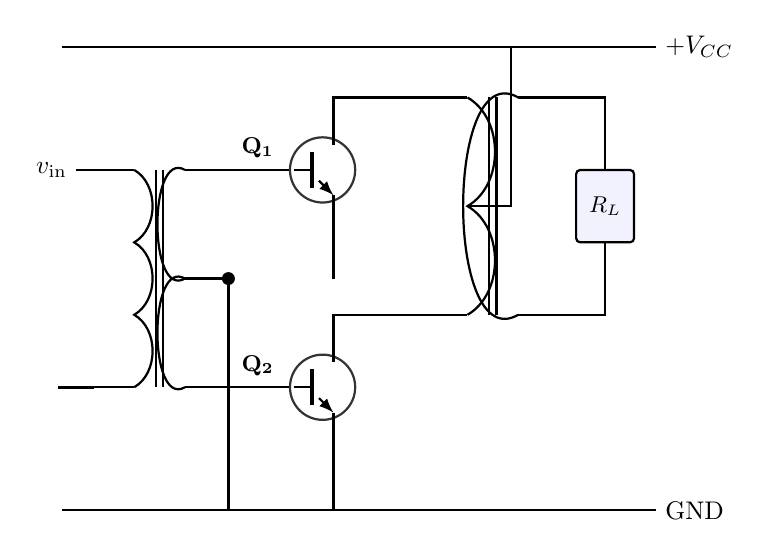
\begin{tikzpicture}[scale=0.92, transform shape]
  % Rails
  \draw[thick] (0, 5.2) -- (8.2, 5.2) node[right] {$+V_{CC}$};
  \draw[thick] (0, -1.2) -- (8.2, -1.2) node[right] {GND};

  % Input Transformer T1
  \draw[thick] (0.2, 3.5) node[left] {$v_{\text{in}}$} -- (1.0, 3.5);
  \draw[thick] (1.0, 3.5) to[out=-30, in=30] (1.0, 2.5) to[out=-30, in=30] (1.0, 1.5) to[out=-30, in=30] (1.0, 0.5);
  \draw[thick] (1.0, 0.5) -- (0.2, 0.5);
  \draw[line width=1.2pt] (-0.05, 0.5) -- (0.45, 0.5);

  % Core T1
  \draw[thick] (1.3, 3.5) -- (1.3, 0.5);
  \draw[thick] (1.4, 3.5) -- (1.4, 0.5);

  % Secondary T1 (Center Tapped)
  \draw[thick] (1.7, 3.5) to[out=150, in=-150] (1.7, 2.0) to[out=150, in=-150] (1.7, 0.5);
  \draw[thick] (1.7, 2.0) -- (2.3, 2.0) node[circle, fill, inner sep=1.8pt] {};
  \draw[thick] (2.3, 2.0) -- (2.3, -1.2);

  % Transistors Q1 and Q2 (NPN)
  \draw[thick] (1.7, 3.5) -- (3.2, 3.5);
  \draw[draw=black!80, fill=white, thick] (3.6, 3.5) circle (0.45cm);
  \draw[line width=1.4pt] (3.45, 3.25) -- (3.45, 3.75);
  \draw[thick] (3.2, 3.5) -- (3.45, 3.5);
  \draw[thick, ->, >=latex] (3.55, 3.35) -- (3.75, 3.15); % Emitter
  \draw[thick] (3.75, 3.15) -- (3.75, 2.0);
  \draw[thick] (3.75, 3.85) -- (3.75, 4.5) -- (5.6, 4.5); % Collector
  \node[left=0.15cm] at (3.2, 3.8) {\small $\mathbf{Q_1}$};

  \draw[thick] (1.7, 0.5) -- (3.2, 0.5);
  \draw[draw=black!80, fill=white, thick] (3.6, 0.5) circle (0.45cm);
  \draw[line width=1.4pt] (3.45, 0.25) -- (3.45, 0.75);
  \draw[thick] (3.2, 0.5) -- (3.45, 0.5);
  \draw[thick, ->, >=latex] (3.55, 0.35) -- (3.75, 0.15); % Emitter
  \draw[thick] (3.75, 0.15) -- (3.75, -1.2);
  \draw[thick] (3.75, 0.85) -- (3.75, 1.5) -- (5.6, 1.5); % Collector
  \node[left=0.15cm] at (3.2, 0.8) {\small $\mathbf{Q_2}$};

  % Output Transformer T2 Primary
  \draw[thick] (5.6, 4.5) to[out=-30, in=30] (5.6, 3.0) to[out=-30, in=30] (5.6, 1.5);
  \draw[thick] (5.6, 3.0) -- (6.2, 3.0) -- (6.2, 5.2);

  % Core T2
  \draw[thick] (5.9, 4.5) -- (5.9, 1.5);
  \draw[thick] (6.0, 4.5) -- (6.0, 1.5);

  % Secondary T2 and Load RL
  \draw[thick] (6.3, 4.5) to[out=150, in=-150] (6.3, 1.5);
  \draw[thick] (6.3, 4.5) -- (7.5, 4.5) -- (7.5, 3.5);
  \draw[thick, fill=blue!5, rounded corners=1.5pt] (7.1, 2.5) rectangle (7.9, 3.5) node[midway] {\small $R_L$};
  \draw[thick] (7.5, 2.5) -- (7.5, 1.5) -- (6.3, 1.5);
\end{tikzpicture}
\end{schematicbox}

\paragraph{Analytical Derivation of General Efficiency:}
\begin{enumerate}[leftmargin=1.5em]
  \item \textbf{AC Output Power ($P_o$):}
  \[
  P_{o(\text{ac})} = \frac{V_p^2}{2 R_L'}
  \]
  \item \textbf{DC Input Power ($P_i$):} The average current drawn from supply $V_{CC}$ across both half cycles is:
  \[
  I_{\text{dc}} = \frac{2}{\pi} I_p = \frac{2}{\pi} \left(\frac{V_p}{R_L'}\right) \implies P_{i(\text{dc})} = V_{CC} I_{\text{dc}} = \frac{2}{\pi} \frac{V_{CC} V_p}{R_L'}
  \]
  \item \textbf{Conversion Efficiency ($\eta$):}
  \[
  \mathbf{\eta = \frac{P_{o(\text{ac})}}{P_{i(\text{dc})}} = \frac{\frac{V_p^2}{2 R_L'}}{\frac{2 V_{CC} V_p}{\pi R_L'}} = \frac{\pi}{4} \left(\frac{V_p}{V_{CC}}\right) \times 100\%}
  \]
  At maximum linear swing ($V_p = V_{CC}$): $\mathbf{\eta_{\max} = \frac{\pi}{4} \approx 78.54\%}$.
\end{enumerate}

\begin{answerbox}
$$\mathbf{\eta = \frac{\pi}{4} \left(\frac{V_p}{V_{CC}}\right) \times 100\%, \qquad \eta_{\max} = 78.54\%}$$
\end{answerbox}

\vspace{0.6cm}

% =========================================================================
% QUESTION 11
% =========================================================================
\subsection{Question 11: Class A Tuned Amplifier 3dB Bandwidth [4 Marks]}
\begin{questionbox}{Problem Statement (2081 Ashwin, Q11)}
Draw the circuit diagram of class A tuned amplifier with its frequency response. Derive its 3dB bandwidth.
\end{questionbox}

\begin{schematicbox}{Class A Tuned Amplifier Circuit and Resonant Response}
\centering
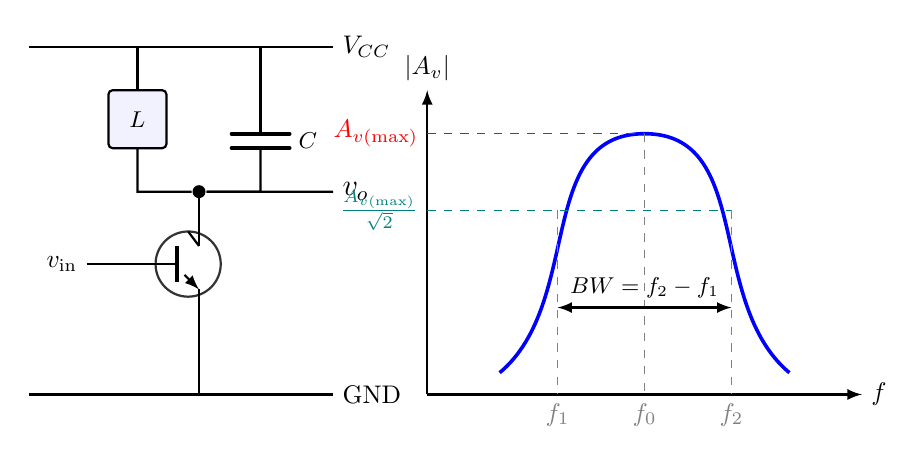
\begin{tikzpicture}[scale=0.92, transform shape]
  % Circuit (Left)
  \draw[thick] (0, 4.8) -- (4.2, 4.8) node[right] {$V_{CC}$};
  \draw[thick] (0, 0) -- (4.2, 0) node[right] {GND};

  % BJT Transistor Q1 (NPN)
  \draw[draw=black!80, fill=white, thick] (2.2, 1.8) circle (0.45cm);
  \draw[line width=1.4pt] (2.05, 1.55) -- (2.05, 2.05); % Base
  \draw[thick] (0.8, 1.8) node[left] {$v_{\text{in}}$} -- (2.05, 1.8);
  \draw[thick] (2.2, 2.25) -- (2.35, 2.05);
  \draw[thick, ->, >=latex] (2.15, 1.65) -- (2.35, 1.45); % Emitter
  \draw[thick] (2.35, 1.45) -- (2.35, 0);

  % Parallel Tuned LC Tank
  \draw[thick] (2.35, 2.05) -- (2.35, 2.8) node[circle, fill, inner sep=1.8pt] (tank_bot) {};
  \draw[thick] (tank_bot) -- (1.5, 2.8) -- (1.5, 3.4);
  \draw[thick, fill=blue!5, rounded corners=1.5pt] (1.1, 3.4) rectangle (1.9, 4.2) node[midway] {\small $L$};
  \draw[thick] (1.5, 4.2) -- (1.5, 4.8);

  \draw[thick] (tank_bot) -- (3.2, 2.8) -- (3.2, 3.4);
  \draw[line width=1.4pt, line cap=round] (2.8, 3.4) -- (3.6, 3.4);
  \draw[line width=1.4pt, line cap=round] (2.8, 3.6) -- (3.6, 3.6);
  \node[right] at (3.6, 3.5) {\small $C$};
  \draw[thick] (3.2, 3.6) -- (3.2, 4.8);

  % Output node
  \draw[thick] (tank_bot) -- (4.2, 2.8) node[right] {\large $v_o$};

  % Resonant Response Curve (Right)
  \draw[thick, ->, >=latex] (5.5, 0) -- (11.5, 0) node[right] {$f$};
  \draw[thick, ->, >=latex] (5.5, 0) -- (5.5, 4.2) node[above] {$|A_v|$};
  \draw[line width=1.3pt, blue] (6.5, 0.3) to[out=40, in=180] (8.5, 3.6) to[out=0, in=140] (10.5, 0.3);

  \draw[dashed, red] (5.5, 3.6) node[left] {$A_{v(\max)}$} -- (8.5, 3.6);
  \draw[dashed, teal] (5.5, 2.54) node[left] {$\frac{A_{v(\max)}}{\sqrt{2}}$} -- (9.7, 2.54);
  \draw[dashed, gray] (7.3, 2.54) -- (7.3, 0) node[below] {$f_1$};
  \draw[dashed, gray] (8.5, 3.6) -- (8.5, 0) node[below] {$f_0$};
  \draw[dashed, gray] (9.7, 2.54) -- (9.7, 0) node[below] {$f_2$};

  \draw[thick, <->, >=latex] (7.3, 1.2) -- (9.7, 1.2) node[midway, above] {\small $BW = f_2 - f_1$};
\end{tikzpicture}
\end{schematicbox}

\paragraph{Derivation of 3dB Bandwidth:}
The resonant frequency of the parallel LC tank is $f_0 = \frac{1}{2\pi\sqrt{LC}}$. The loaded quality factor $Q$ is defined as $Q = \frac{R_p}{\omega_0 L} = \omega_0 C R_p$.\\
The $3\text{dB}$ bandwidth between lower ($f_1$) and upper ($f_2$) half-power cutoff frequencies is:
\[
\mathbf{BW = f_2 - f_1 = \frac{f_0}{Q} = \frac{1}{2\pi R_p C}}
\]

\begin{answerbox}
$$\mathbf{BW = \frac{f_0}{Q} = \frac{1}{2\pi R_p C}}$$
\end{answerbox}

\vspace{0.6cm}

% =========================================================================
% QUESTION 12
% =========================================================================
\subsection{Question 12: LM317 Variable DC Regulator Design (10V - 20V) [4 Marks]}
\begin{questionbox}{Problem Statement (2081 Ashwin, Q12)}
Design variable DC voltage regulator using LM 317 to get $(10-20)\text{ volts}$ output.
\end{questionbox}

\[
V_{\text{out}} = 1.25\text{V} \left(1 + \frac{R_2}{R_1}\right)
\]
\begin{enumerate}[leftmargin=1.5em]
  \item Select standard $R_1 = \mathbf{240\ \Omega}$.
  \item For $V_{\text{out}(\min)} = 10.0\text{V}$:
  \[
  10.0 = 1.25 \left(1 + \frac{R_{2(\min)}}{240}\right) \implies R_{2(\min)} = 7.0 \times 240 = \mathbf{1680\ \Omega} = \mathbf{1.68\text{ k}\Omega}
  \]
  \item For $V_{\text{out}(\max)} = 20.0\text{V}$:
  \[
  20.0 = 1.25 \left(1 + \frac{R_{2(\max)}}{240}\right) \implies R_{2(\max)} = 15.0 \times 240 = \mathbf{3600\ \Omega} = \mathbf{3.60\text{ k}\Omega}
  \]
\end{enumerate}
\textbf{Implementation:} Use a fixed resistor $R_{2A} = 1.6\text{ k}\Omega$ in series with a $\mathbf{2.0\text{ k}\Omega}$ linear potentiometer ($R_2 = 1.68\text{ k}\Omega \text{ to } 3.60\text{ k}\Omega$). Input voltage: $V_{\text{in}} \ge 23\text{V DC}$.

\begin{answerbox}
$$\mathbf{R_1 = 240\ \Omega, \qquad R_2 = 1.68\text{ k}\Omega \text{ to } 3.60\text{ k}\Omega \quad (\text{Fixed } 1.6\text{k}\Omega + 2.0\text{k}\Omega \text{ Potentiometer})}$$
\end{answerbox}

\vspace{0.6cm}

% =========================================================================
% QUESTION 13
% =========================================================================
\subsection{Question 13: Series Transistor Regulator with Error Amplifier \& Stability Factor [2 + 2 = 4 Marks]}
\begin{questionbox}{Problem Statement (2081 Ashwin, Q13)}
Explain the working principle of a series transistor voltage regulator with improved performance and derive an expression for the voltage stability.
\end{questionbox}

\begin{schematicbox}{Series Voltage Regulator with Op-Amp / BJT Error Amplifier}
\centering
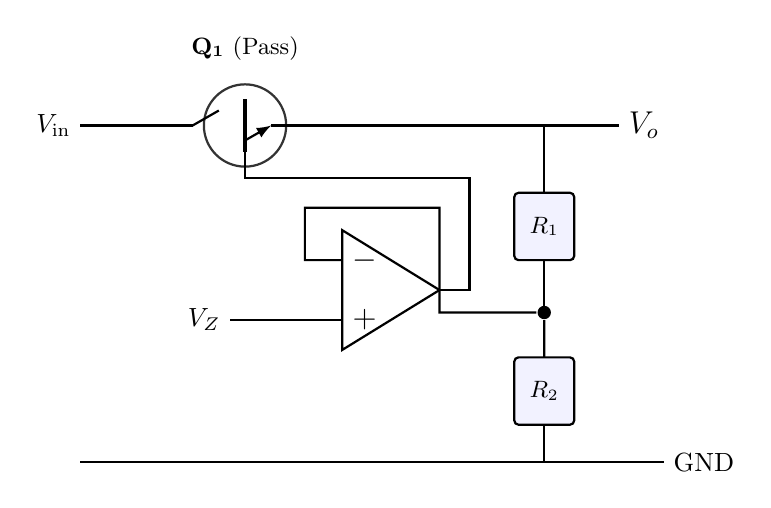
\begin{tikzpicture}[scale=0.95, transform shape]
  % Rails
  \draw[thick] (0, 4.5) node[left] {$V_{\text{in}}$} -- (1.5, 4.5);
  \draw[thick] (0, 0) -- (7.8, 0) node[right] {GND};

  % Pass Transistor Q1 (NPN)
  \draw[draw=black!80, fill=white, thick] (2.2, 4.5) circle (0.55cm);
  \draw[line width=1.6pt] (2.2, 4.15) -- (2.2, 4.85); % Base
  \draw[thick] (1.5, 4.5) -- (1.85, 4.7); % Collector
  \draw[thick, ->, >=latex] (2.2, 4.3) -- (2.55, 4.5); % Emitter
  \draw[thick] (2.55, 4.5) -- (7.2, 4.5) node[right] {\large $V_o$};
  \node[above=0.2cm] at (2.2, 5.05) {\small $\mathbf{Q_1}$ (Pass)};

  % Voltage Divider Sampling Network (R1, R2)
  \draw[thick] (6.2, 4.5) -- (6.2, 3.6);
  \draw[thick, fill=blue!5, rounded corners=1.5pt] (5.8, 2.7) rectangle (6.6, 3.6) node[midway] {\small $R_1$};
  \draw[thick] (6.2, 2.7) -- (6.2, 2.0) node[circle, fill, inner sep=1.8pt] (vsample) {};
  \draw[thick] (vsample) -- (6.2, 1.4);
  \draw[thick, fill=blue!5, rounded corners=1.5pt] (5.8, 0.5) rectangle (6.6, 1.4) node[midway] {\small $R_2$};
  \draw[thick] (6.2, 0.5) -- (6.2, 0);

  % Error Amplifier (Op-Amp)
  \draw[thick, fill=white] (3.5, 1.5) -- (3.5, 3.1) -- (4.8, 2.3) -- cycle;
  \node at (3.8, 2.7) {\large $-$};
  \node at (3.8, 1.9) {\large $+$};

  % Inverting input samples Vo
  \draw[thick] (vsample) -- (4.8, 2.0) -- (4.8, 3.4) -- (3.0, 3.4) -- (3.0, 2.7) -- (3.5, 2.7);
  % Non-inverting input receives VZ
  \draw[thick] (2.0, 1.9) node[left] {$V_Z$} -- (3.5, 1.9);
  % Output controls Pass Transistor Base
  \draw[thick] (4.8, 2.3) -- (5.2, 2.3) -- (5.2, 3.8) -- (2.2, 3.8) -- (2.2, 4.15);
\end{tikzpicture}
\end{schematicbox}

An improved series regulator incorporates an active error amplifier (Op-Amp or BJT $Q_2$) comparing a sampled fraction of the output $\beta_s V_o = \frac{R_2}{R_1+R_2}V_o$ against reference voltage $V_Z$.
\begin{itemize}[leftmargin=1.5em]
  \item \textbf{Operation:} If $V_o$ increases due to input or load variations, $V_{\text{sample}}$ increases above $V_Z$, causing the error amplifier output to pull down the base potential of pass transistor $Q_1$, decreasing $V_o$ back to the set level.
  \item \textbf{Voltage Stability Factor ($S_V$):}
  \[
  \mathbf{S_V = \frac{\Delta V_o}{\Delta V_{\text{in}}} = \frac{r_z}{R + r_z} \cdot \frac{1}{1 + A_{\text{error}} \beta_s} \approx \frac{r_z}{R \cdot A_{\text{error}} \beta_s}}
  \]
  The high open-loop gain $A_{\text{error}}$ of the error amplifier suppresses input line fluctuations by several orders of magnitude.
\end{itemize}

\begin{answerbox}
$$\mathbf{S_V = \frac{\Delta V_o}{\Delta V_{\text{in}}} \approx \frac{r_z}{R \cdot A_{\text{error}} \beta_s}}$$
\end{answerbox}

\end{document}
